% Options for packages loaded elsewhere
\PassOptionsToPackage{unicode}{hyperref}
\PassOptionsToPackage{hyphens}{url}
\PassOptionsToPackage{dvipsnames,svgnames,x11names}{xcolor}
%
\documentclass[
]{scrbook}
\usepackage{amsmath,amssymb}
\usepackage{iftex}
\ifPDFTeX
  \usepackage[T1]{fontenc}
  \usepackage[utf8]{inputenc}
  \usepackage{textcomp} % provide euro and other symbols
\else % if luatex or xetex
  \usepackage{unicode-math} % this also loads fontspec
  \defaultfontfeatures{Scale=MatchLowercase}
  \defaultfontfeatures[\rmfamily]{Ligatures=TeX,Scale=1}
\fi
\usepackage{lmodern}
\ifPDFTeX\else
  % xetex/luatex font selection
\fi
% Use upquote if available, for straight quotes in verbatim environments
\IfFileExists{upquote.sty}{\usepackage{upquote}}{}
\IfFileExists{microtype.sty}{% use microtype if available
  \usepackage[]{microtype}
  \UseMicrotypeSet[protrusion]{basicmath} % disable protrusion for tt fonts
}{}
\makeatletter
\@ifundefined{KOMAClassName}{% if non-KOMA class
  \IfFileExists{parskip.sty}{%
    \usepackage{parskip}
  }{% else
    \setlength{\parindent}{0pt}
    \setlength{\parskip}{6pt plus 2pt minus 1pt}}
}{% if KOMA class
  \KOMAoptions{parskip=half}}
\makeatother
\usepackage{xcolor}
\usepackage{longtable,booktabs,array}
\usepackage{calc} % for calculating minipage widths
% Correct order of tables after \paragraph or \subparagraph
\usepackage{etoolbox}
\makeatletter
\patchcmd\longtable{\par}{\if@noskipsec\mbox{}\fi\par}{}{}
\makeatother
% Allow footnotes in longtable head/foot
\IfFileExists{footnotehyper.sty}{\usepackage{footnotehyper}}{\usepackage{footnote}}
\makesavenoteenv{longtable}
\usepackage{graphicx}
\makeatletter
\def\maxwidth{\ifdim\Gin@nat@width>\linewidth\linewidth\else\Gin@nat@width\fi}
\def\maxheight{\ifdim\Gin@nat@height>\textheight\textheight\else\Gin@nat@height\fi}
\makeatother
% Scale images if necessary, so that they will not overflow the page
% margins by default, and it is still possible to overwrite the defaults
% using explicit options in \includegraphics[width, height, ...]{}
\setkeys{Gin}{width=\maxwidth,height=\maxheight,keepaspectratio}
% Set default figure placement to htbp
\makeatletter
\def\fps@figure{htbp}
\makeatother
\setlength{\emergencystretch}{3em} % prevent overfull lines
\providecommand{\tightlist}{%
  \setlength{\itemsep}{0pt}\setlength{\parskip}{0pt}}
\setcounter{secnumdepth}{5}
% definitions for citeproc citations
\NewDocumentCommand\citeproctext{}{}
\NewDocumentCommand\citeproc{mm}{%
  \begingroup\def\citeproctext{#2}\cite{#1}\endgroup}
\makeatletter
 % allow citations to break across lines
 \let\@cite@ofmt\@firstofone
 % avoid brackets around text for \cite:
 \def\@biblabel#1{}
 \def\@cite#1#2{{#1\if@tempswa , #2\fi}}
\makeatother
\newlength{\cslhangindent}
\setlength{\cslhangindent}{1.5em}
\newlength{\csllabelwidth}
\setlength{\csllabelwidth}{3em}
\newenvironment{CSLReferences}[2] % #1 hanging-indent, #2 entry-spacing
 {\begin{list}{}{%
  \setlength{\itemindent}{0pt}
  \setlength{\leftmargin}{0pt}
  \setlength{\parsep}{0pt}
  % turn on hanging indent if param 1 is 1
  \ifodd #1
   \setlength{\leftmargin}{\cslhangindent}
   \setlength{\itemindent}{-1\cslhangindent}
  \fi
  % set entry spacing
  \setlength{\itemsep}{#2\baselineskip}}}
 {\end{list}}
\usepackage{calc}
\newcommand{\CSLBlock}[1]{\hfill\break\parbox[t]{\linewidth}{\strut\ignorespaces#1\strut}}
\newcommand{\CSLLeftMargin}[1]{\parbox[t]{\csllabelwidth}{\strut#1\strut}}
\newcommand{\CSLRightInline}[1]{\parbox[t]{\linewidth - \csllabelwidth}{\strut#1\strut}}
\newcommand{\CSLIndent}[1]{\hspace{\cslhangindent}#1}
\ifLuaTeX
\usepackage[bidi=basic]{babel}
\else
\usepackage[bidi=default]{babel}
\fi
\babelprovide[main,import]{ngerman}
% get rid of language-specific shorthands (see #6817):
\let\LanguageShortHands\languageshorthands
\def\languageshorthands#1{}
\addtokomafont{disposition}{\rmfamily}
\KOMAoptions{numbers=noenddot}

\usepackage{libertine}
\usepackage{libertinus-otf}

\usepackage[original]{imakeidx}
% \usepackage{makeidx}
% \makeindex[title=Stichwortverzeichnis, intoc]
% \indexsetup{level=\chapter,toclevel=chapter,noclearpage,firstpagestyle=headings}



\usepackage{color}
\definecolor{formalColor}{HTML}{00A2FF}
\definecolor{semanticColor}{HTML}{1DB100}
\definecolor{concreteColor}{HTML}{EE220C}
\definecolor{empiricColor}{HTML}{F8BA00}
\definecolor{linkColor}{HTML}{929292}
\definecolor{quoteColor}{HTML}{666666}

\usepackage{framed}
\renewenvironment{quote}{
  \list{}{
	\leftmargin0.2cm   % this is the adjusting screw
    \rightmargin\leftmargin
      	\def\FrameCommand
    {%
        {\color{quoteColor}\vrule width 2pt}%
        \hspace{0pt}%must no space.
        %
    }%
    \MakeFramed{\advance \hsize -\width \FrameRestore}    \color{quoteColor}
    }
  \item\relax
}
{\endlist\color{black}\endMakeFramed}


\makeatletter
\def\renewtheorem#1{%
  \expandafter\let\csname#1\endcsname\relax
  \expandafter\let\csname c@#1\endcsname\relax
  \gdef\renewtheorem@envname{#1}
  \renewtheorem@secpar
}
\def\renewtheorem@secpar{\@ifnextchar[{\renewtheorem@numberedlike}{\renewtheorem@nonumberedlike}}
\def\renewtheorem@numberedlike[#1]#2{\newtheorem{\renewtheorem@envname}[#1]{#2}}
\def\renewtheorem@nonumberedlike#1{
\def\renewtheorem@caption{#1}
\edef\renewtheorem@nowithin{\noexpand\newtheorem{\renewtheorem@envname}{\renewtheorem@caption}}
\renewtheorem@thirdpar
}
\def\renewtheorem@thirdpar{\@ifnextchar[{\renewtheorem@within}{\renewtheorem@nowithin}}
\def\renewtheorem@within[#1]{\renewtheorem@nowithin[#1]}
\makeatother
\ifLuaTeX
  \usepackage{selnolig}  % disable illegal ligatures
\fi
\usepackage{bookmark}
\IfFileExists{xurl.sty}{\usepackage{xurl}}{} % add URL line breaks if available
\urlstyle{same}
\hypersetup{
  pdftitle={Stoffdidaktik Mathematik -- Skript zur Vorlesung im Wintersemester 2024/25},
  pdfauthor={Dr.~Heiko Etzold, Universität Potsdam},
  pdflang={de-DE},
  colorlinks=true,
  linkcolor={linkColor},
  filecolor={Maroon},
  citecolor={Blue},
  urlcolor={linkColor},
  pdfcreator={LaTeX via pandoc}}

\title{Stoffdidaktik Mathematik -- Skript zur Vorlesung im Wintersemester 2024/25}
\author{Dr.~Heiko Etzold, Universität Potsdam}
\date{Letzte Änderung: 16.11.2024}

\usepackage{amsthm}
\newtheorem{theorem}{Theorem}[chapter]
\newtheorem{lemma}{Lemma}[chapter]
\newtheorem{corollary}{Corollary}[chapter]
\newtheorem{proposition}{Proposition}[chapter]
\newtheorem{conjecture}{Conjecture}[chapter]
\theoremstyle{definition}
\newtheorem{definition}{Definition}[chapter]
\theoremstyle{definition}
\newtheorem{example}{Example}[chapter]
\theoremstyle{definition}
\newtheorem{exercise}{Exercise}[chapter]
\theoremstyle{definition}
\newtheorem{hypothesis}{Hypothesis}[chapter]
\theoremstyle{remark}
\newtheorem*{remark}{Remark}
\newtheorem*{solution}{Solution}
\begin{document}
\maketitle

% \renewtheorem{definition}{Definition}[chapter]
%
% \newtheoremstyle{definition}% name of the style to be used
% {}% measure of space to leave above the theorem. E.g.: 3pt
% {}% measure of space to leave below the theorem. E.g.: 3pt
% {\em}% name of font to use in the body of the theorem
% {}% measure of space to indent
% {\bf}% name of head font
% {.}% punctuation between head and body
% { }% space after theorem head; " " = normal interword space
% {\thmname{#1}\thmnumber{\addtocounter{thm}{-1} #2$^\prime$}\thmnote{\textnormal{ (#3)}}}

{
\hypersetup{linkcolor=}
\setcounter{tocdepth}{1}
\tableofcontents
}
\chapter*{Über dieses Dokument}\label{uxfcber-dieses-dokument}
\addcontentsline{toc}{chapter}{Über dieses Dokument}

Die Veranstaltung \emph{Stoffdidaktik Mathematik} wird über dieses Dokument begleitet. Es wird fortlaufend aktualisiert und zur Verfügung gestellt. Über ein Git-Respository können Änderungen nachverfolgt werden.
In der html-Version gelangt man über die Menüleiste am oberen Rand sowohl zu den Rohdaten als auch zu einer pdf-Version. Die Darstellung der Inhalte ist jedoch optimiert für die html-Version dieses Dokuments.

Aufgrund der permanenten Entwicklung ist eine Zitation des aktuellen Skriptes nicht unbedingt geeignet. Sollte ein Verweis notwendig sein, wird als Quellenangabe empfohlen:

\begin{quote}
Etzold, H. (2024). \emph{Stoffdidaktik Mathematik -- Skript zur Vorlesung im Wintersemester 2024/25} (Version vom 16.11.2024). \url{https://stoffdidaktik.heiko-etzold.de}
\end{quote}

Die Vorlesungsskripte der letztjährigen Veranstaltungen, die sich dann auch zur Zitation eignen, finden Sie unter:

\begin{itemize}
\tightlist
\item
  \url{https://stoffdidaktik.heiko-etzold.de/2023}
\item
  \url{https://stoffdidaktik.heiko-etzold.de/2022}
\item
  \url{https://stoffdidaktik.heiko-etzold.de/2021}
\end{itemize}

\section*{Lizenz}\label{lizenz}

Soweit nicht anders gekennzeichnet, ist dieses Dokument unter einem Creative Commons Lizenzvertrag lizenziert: »Namensnennung -- Weitergabe unter gleichen Bedingungen 4.0 International«. Dies gilt nicht für Zitate und Werke, die aufgrund einer anderen Erlaubnis genutzt werden.
Eine Beschreibung der Lizenz findet sich unter \url{https://creativecommons.org/licenses/by-sa/4.0/deed.de}.

\chapter*{Stoffdidaktik Mathematik an der UP}\label{stoffdidaktik-mathematik-an-der-up}
\addcontentsline{toc}{chapter}{Stoffdidaktik Mathematik an der UP}

\section*{Struktur der Veranstaltung}\label{struktur-der-veranstaltung}
\addcontentsline{toc}{section}{Struktur der Veranstaltung}

Die Veranstaltung \emph{Stoffdidaktik Mathematik}\footnote{Die Modulbeschreibung finden Sie bei \href{https://puls.uni-potsdam.de/qisserver/rds?state=verpublish&status=init&vmfile=no&moduleCall=modulansicht&publishConfFile=modulverwaltung&publishSubDir=up/modulbearbeiter&&modul.modul_id=3155&menuid=&topitem=Modulbeschreibung&subitem=}{PULS}.} besteht aus einer \textbf{Vorlesung (2~SWS)} und einem zugehörigen \textbf{Seminar (2~SWS)}.

Im Wintersemester 2024/25 wird die \textbf{Vorlesung semesterbegleitend} stattfinden. Das \textbf{Seminar} können Sie entweder \textbf{parallel zur Vorlesung} im Wintersemester oder \textbf{semesterbegleitend} im Sommersemester 2025 besuchen.

In der Vorlesung erhalten Sie einen \textbf{Input zu stoffdidaktischen Grundlagen}, wobei der Schwerpunkt auf \textbf{stoffdidaktischen Theorien} liegt, die über vielfältige Unterrichtsbeispiele illustriert werden. Im Seminar haben Sie die Aufgabe, diese Grundlagen selbstständig \textbf{auf verschiedene Lerngegenstände anzuwenden}.

Sie halten einen \textbf{Seminarvortrag} (30 bis 45 Minuten) als Voraussetzung für die Zulassung zur Modulprüfung und fassen Ihre Erarbeitungen in einer \textbf{Hausarbeit} (6 bis 8 Seiten) zusammen, die als Modulprüfung dient.

\section*{Einordnung}\label{einordnung}
\addcontentsline{toc}{section}{Einordnung}

Die Veranstaltung \emph{Stoffdidaktik Mathematik} findet nach empfohlenem Studienverlaufsplan im \textbf{5. Fachsemester parallel zur \emph{Einführung in die Mathematikdidaktik}} statt.

Das heißt insbesondere, dass Sie bereits die \textbf{Grundlagen} zur Analysis, Linearen Algebra, Stochastik, Geometrie, Algebra und Numerik studiert haben sollten. Auf diese Grundlagen wird in der Stoffdidaktisch \textbf{fachlich aufgebaut}.

Während Sie sich in der \emph{Einführung in die Mathematikdidaktik} mit verschiedenen Lehr-Lern-Theorien, Unterrichtsprinzipien, prozessbezogenen Kompetenzen oder methodischen Grundlagen des Mathematikunterrichtens beschäftigen, liegt in der \emph{Stoffdidaktik Mathematik} der Fokus auf der \textbf{Auswahl und Strukturierung der Unterrichtsinhalte}, basierend auf fachlichen und fachdidaktischen Erkenntnissen.

Parallel oder im Anschluss an beide Veranstaltungen absolvieren Sie das \textbf{fachdidaktische Tagespraktikum}, in dem Sie die erworbenen Kenntnisse in die \textbf{Unterrichtspraxis} transferieren und erste eigene Unterrichtsstunden im Fach Mathematik halten.

\section*{Kompetenzziele der Veranstaltung}\label{kompetenzziele-der-veranstaltung}
\addcontentsline{toc}{section}{Kompetenzziele der Veranstaltung}

Als Kompetenzen, die Sie nach Abschluss von Vorlesung und Seminar erreicht haben sollen, sind angedacht:

\begin{itemize}
\tightlist
\item
  Sie \textbf{kennen Aspekte und Grundvorstellungen} zu zentralen mathematischen Begriffen.
\item
  Sie \textbf{beurteilen Unterrichtsmaterialien und Lernumgebungen} hinsichtlich ihrer stoffdidaktischen Eignung.
\item
  Sie \textbf{erstellen Aufgaben und erste Lernumgebungen} zu konkreten Stoffgebieten.
\item
  Sie \textbf{erkennen mathematikdidaktische Prinzipien und Ideen} als \textbf{Entscheidungs- und Strukturierungsgrundlage} zu stofflichen Inhalten der mathematischen Bildung.
\item
  Sie \textbf{wählen zielgerichtet} analoge und digitale \textbf{Medien} zur Unterstützung stofflich orientierter Lehr-Lern-Prozesse aus.
\item
  Sie \textbf{setzen sich} selbstständig \textbf{mit stoffdidaktischen Fragestellungen auseinander} und nutzen dafür geeignete mathematikdidaktische Literatur.
\item
  Sie \textbf{reflektieren die Inhalte der vorangegangenen Mathematik-Fachmodule} unter stoffdidaktischen Gesichtspunkten.
\end{itemize}

\section*{Was ist Stoffdidaktik?}\label{was-ist-stoffdidaktik}
\addcontentsline{toc}{section}{Was ist Stoffdidaktik?}

Für die Disziplin der \emph{Stoffdidaktik Mathematik} gibt es keine allgemeingültige Definition, auch haben sich die Schwerpunkte in der historischen Entwicklung stets verschoben.

Grundsätzliches Ziel ist, stoffliche Inhaltsbereiche für den Mathematikunterricht auszuwählen (\textbf{\emph{Was?}}) und aufzubereiten (\textbf{\emph{Wie?}}). Im Sinne dieser Veranstaltung kann Stoffdidaktik grob als \textbf{Spezifierung und Strukturierung von Lerngegenständen} aufgefasst werden (zur begrifflichen Einordnung siehe auch \citeproc{ref-Hussmann:2016a}{Hußmann et al., 2016}).

Während hierzu, historisch betrachtet, anfangs der Stoff ausschließlich aus fachmathematischer Perspektive aufbereitet wurde (z.~B. durch \emph{didaktisch-orientierte Sachanalysen}), nahmen in der Folgezeit mehr und mehr auch Lehr-Lern-Theorien Einzug -- gar ein Verschwinden der stofflichen Orientierung der Mathematikdidaktik wird befürchtet (vgl. \citeproc{ref-Jahnke:2010}{Jahnke, 2010}).

Mit dem Begriff der \textbf{Strukturgenetischen Analyse} erweitert Wittmann (\citeproc{ref-Wittmann:2015}{2015}) die historische Sichtweise als eine »Mathematikdidaktik \emph{vom Fach aus}«, die sich »auf implizite Theorien des Lehrens und Lernens, die im Fach selbst liegen{[}, stützt{]}« (\citeproc{ref-Wittmann:2015}{Wittmann, 2015, S. 240}). »Anders als bei der Stoffdidaktik, die sich im Wesentlichen auf die logische Analyse des Stoffes und die Wissensvermittlung konzentriert hat, stehen jetzt aber die Genese des Wissens im Verlauf der Schulzeit und Lernprozesse unter Bezug auf unterschiedliche Lernvoraussetzungen im Vordergrund« (\citeproc{ref-Wittmann:2015}{Wittmann, 2015, S. 250}). Eine derartig ganzheitliche Sichtweise soll auch den Geist dieser Veranstaltung ausmachen.

\begin{quote}
\textbf{Überblicke zur historischen Entwicklung der Stoffdidaktik}

\begin{itemize}
\tightlist
\item
  Hefendehl-Hebeker (\citeproc{ref-Hefendehl-Hebeker:2016}{2016}): Subject-matter didactics in German traditions: Early historical developments
\item
  Schupp (\citeproc{ref-Schupp:2016}{2016, 79~ff.}): Gedanken zum „Stoff`` und zur „Stoffdidaktik`` sowie zu ihrer Bedeutung für die Qualität des Mathematikunterrichts
\end{itemize}
\end{quote}

\part*{Stoffdidaktische Analyse}\label{part-stoffdidaktische-analyse}
\addcontentsline{toc}{part}{Stoffdidaktische Analyse}

\chapter{Vier-Ebenen-Ansatz}\label{vier-ebenen-ansatz}

\begin{quote}
\textbf{Ziele}

\begin{itemize}
\tightlist
\item
  Sie kennen typische Fragestellungen, um sich einer stoffdidaktischen Analyse systematisch zu nähern.
\item
  Sie erkennen den Vier-Ebenen-Ansatz als eine Möglichkeit, eine stoffdidaktische Analyse strukturiert vorzunehmen.
\item
  Sie können den Vier-Ebenen-Ansatz anhand eines Beispiels nachvollziehen.
\item
  Sie sind sich der Komplexität einer stoffdidaktischen Analyse bewusst.
\end{itemize}

\textbf{Material}

\begin{itemize}
\tightlist
\item
  Folien zum Kapitel 1 (\href{files/Stoffdidaktik2024-01-VierEbenenAnsatz.pdf}{pdf}, \href{files/Stoffdidaktik2024-01-VierEbenenAnsatz.key}{Keynote})
\item
  \href{https://apps.apple.com/de/app/winkel-farm/id1369585218}{App \emph{Winkel-Farm}} (nur für iOS)
\end{itemize}
\end{quote}

\section{Analyse von Lerngegenständen}\label{analyse-von-lerngegenstuxe4nden}

Die inhaltliche Basis der ersten Kapitel dieses Skriptes bietet ein Beitrag von Hußmann \& Prediger (\citeproc{ref-Hussmann:2016}{2016}) zur Spezifizierung und Strukturierung mathematischer Lerngegenstände. Dieser Beitrag schlägt eine Kategorisierung stoffdidaktischer Analysen vor und formuliert vielfältige Fragen, woraus sich wieder ein ganzes Repertoir an Themen ergibt, die es im Rahmen der Stoffdidaktik-Veranstaltung zu untersuchen gilt.

Hußmann \& Prediger (\citeproc{ref-Hussmann:2016}{2016, 35~f.})\index{4-Ebenen-Ansatz|see{Vier-Ebenen-Ansatz}} kategorisieren eine stoffdidaktische Analyse in eine \textbf{\textcolor{formalColor}{formale}}, \textbf{\textcolor{semanticColor}{semantische}}, \textbf{\textcolor{concreteColor}{konkrete}} und \textbf{\textcolor{empiricColor}{empirische}} Ebene, wobei diese nicht hierarchisch aufgebaut sind, sondern sich gegenseitig beeinflussen. Innerhalb der Ebenen wird jeweils noch einmal in die \textbf{Spezifizierung} und die \textbf{Strukturierung} eines Lerngegenstands unterschieden.

Auf der \textcolor{formalColor}{formalen Ebene}\index{Vier-Ebenen-Ansatz!formale Ebene|textbf} wird der Lerngegenstand aus seiner fachlich-logischen Struktur heraus betrachtet.

Die \textcolor{semanticColor}{semantische Ebene}\index{Vier-Ebenen-Ansatz!semantische Ebene|textbf} adressiert Sinn und Bedeutung des mathematischen Gegenstands sowie erkenntnistheoretische Aspekte.

Ziel der \textcolor{concreteColor}{konkreten Ebene}\index{Vier-Ebenen-Ansatz!konkrete Ebene|textbf} ist die Umsetzung des Lehr-Lern-Prozesses an konkreten Situationen, über die das mathematische Wissen konstruiert wird.

Über die \textcolor{empiricColor}{empirische Ebene}\index{Vier-Ebenen-Ansatz!empirische Ebene|textbf} werden die kognitiven und ggf. sozialen Aspekte der Schülerinnen und Schüler in die stoffdidaktische Analyse integriert.

Über die \textbf{Spezifizierung} wird ermittelt, \emph{was} genau Schülerinnen und Schüler bezüglich eines bestimmten mathematischen Themas lernen sollen, während die \textbf{Strukturierung} analysiert, \emph{wie} diese Elemente miteinander in Verbindung stehen und wie sie im Lernpfad strukturiert werden können.

Aus den vier Ebenen und der jeweiligen Unterscheidung in Spezifizierung und Strukturierung ergeben sich acht (nicht immer trennscharfe) Dimensionen, die den Analyseprozess zu einem Lerngegenstand kategorisieren können. Um dies für Forschungs- und Entwicklungsprozesse greifbar zu machen, haben Hußmann \& Prediger (\citeproc{ref-Hussmann:2016}{2016, S. 36}) typische Fragestellungen formuliert, an die in Tabelle \ref{tab:fragen-ebenen} mehr oder weniger stark angelehnt wird.

\begin{longtable}[]{@{}
  >{\raggedright\arraybackslash}p{(\columnwidth - 4\tabcolsep) * \real{0.2857}}
  >{\raggedright\arraybackslash}p{(\columnwidth - 4\tabcolsep) * \real{0.3571}}
  >{\raggedright\arraybackslash}p{(\columnwidth - 4\tabcolsep) * \real{0.3571}}@{}}
\caption{\label{tab:fragen-ebenen} Typische Fragestellungen, angelehnt an Hußmann \& Prediger (\citeproc{ref-Hussmann:2016}{2016, S. 36})}\tabularnewline
\toprule\noalign{}
\begin{minipage}[b]{\linewidth}\raggedright
\end{minipage} & \begin{minipage}[b]{\linewidth}\raggedright
Spezifizierung
\end{minipage} & \begin{minipage}[b]{\linewidth}\raggedright
Strukturierung
\end{minipage} \\
\midrule\noalign{}
\endfirsthead
\toprule\noalign{}
\begin{minipage}[b]{\linewidth}\raggedright
\end{minipage} & \begin{minipage}[b]{\linewidth}\raggedright
Spezifizierung
\end{minipage} & \begin{minipage}[b]{\linewidth}\raggedright
Strukturierung
\end{minipage} \\
\midrule\noalign{}
\endhead
\bottomrule\noalign{}
\endlastfoot
\textbf{\textcolor{formalColor}{Formale Ebene}} & \textbf{Welche Begriffe, Zusammenhänge und Verfahren} sollen erarbeitet werden? Wie können die Zusammenhänge und Verfahren \textbf{formal begründet} werden? & Wie kann das \textbf{Netzwerk} aus Begriffen, Zusammenhängen und Verfahren \textbf{logisch strukturiert} werden? Welche \textbf{Verbindungen} zwischen den Fachinhalten sind aus fachlicher Perspektive entscheidend, welche weniger? \\
\textbf{\textcolor{semanticColor}{Semantische Ebene}} & \textbf{Welche} (mathematisch-gesellschaftliche) \textbf{Bedeutung} liegt hinter dem Lerngegenstand (vgl. \hyperref[fundamentale-ideen]{\emph{Fundamentale Ideen}})? \textbf{Welcher Sinn} soll bei den Schülerinnen und Schülern hinsichtlich des Lerngegenstands aufgedeckt werden und \textbf{welche Repräsentationen} sind dafür geeignet (vgl. \hyperref[grundvorstellungen]{\emph{Grundvorstellungen}})? & Wie \textbf{verhalten} sich Sinn und Bedeutung des Lerngegenstands \textbf{zueinander} und \textbf{zu früheren und späteren Lerngegenständen}? \\
\textbf{\textcolor{concreteColor}{Konkrete Ebene}} & \textbf{Welche \hyperref[kernidee-begriffsklaerung]{Kernfragen und Kernideen}} können die Entwicklung der Begriffe, Zusammenhänge und Verfahren leiten? \textbf{Welche} (inner- und außermathematischen) \textbf{\hyperref[kontexte-begriffsklaerung]{Kontexte}} sind geeignet, um an ihnen die Kernfragen und -ideen exemplarisch zu behandeln und die Inhalte zu rekonstruieren? & Wie kann das Verständnis sukzessive \textbf{über realitätsbezogene Situationen} in dem beabsichtigten Lernpfad konstruiert werden (vgl. \hyperref[mathematisierungstypen]{\emph{horizontale Mathematisierung}})? Wie kann der Lernpfad \textbf{in Bezug auf die mathematische Problemstruktur} angeordnet werden (vgl. \hyperref[mathematisierungstypen]{\emph{vertikale Mathematisierung}})? \\
\textbf{\textcolor{empiricColor}{Empirische Ebene}} & \textbf{Welche} typischen \textbf{individuellen Voraussetzungen} (Vorstellungen, Kenntnisse, Kompetenzen, \ldots) sind zu erwarten und \textbf{wie passen} diese zum \textbf{angestrebten Verständnis}? \textbf{Woher} kommen typische \textbf{Hindernisse} oder \textbf{unerwünschte Vorstellungen}? & Wie können typische \textbf{Vorkenntnisse und Vorstellungen} als \textbf{fruchtbare Anknüpfungspunkte} dienen? Welche \textbf{Schlüsselstellen} (Hindernisse, Wendepunkte, \ldots) gibt es \textbf{im Lernweg} der Schülerinnen und Schüler? \\
\end{longtable}

Diese Fragen können dabei helfen, einen Lerngegenstand aus professioneller Sicht vollumfänglich zu analysieren (insb. Spezifizierung) und daraus die Gestaltung eines Lernpfades für Schülerinnen und Schüler abzuleiten (insb. Strukturierung). Noch \emph{nicht} abgeleitet werden kann daraus jedoch die Gestaltung einer \emph{konkreten Unterrichtsstunde} -- dies bedarf weiterer Überlegungen, z.~B. zu Unterrichtsmethoden, Aufgaben, Klassenmanagement, \ldots{} (\citeproc{ref-Hussmann:2016}{Hußmann \& Prediger, 2016, S. 37}).

\section{Lernbereich und Lerngegenstand}\label{lernbereich-und-lerngegenstand}

Als \textbf{\emph{Lerngegenstände}} werden im Rahmen dieser Veranstaltung für spezifische Ausbildungszwecke ausgewählte Ausschnitte des gesellschaftlichen Wissens und Könnens angesehen (vgl. \citeproc{ref-Lompscher1985b}{Lompscher, 1985}). Diese Sichtweise entstammt tätigkeitstheoretischen Überlegungen, wobei zwischen gesellschaftlichem Wissen und Können und individuellen Kenntnissen, Fähigkeiten und Fertigkeiten unterschieden wird. Weitere Hintergrundinformationen dazu finden Sie in späteren Kapiteln.

Zu Lerngegenständen gehören -- im Rahmen des Mathematikunterrichts -- sowohl \textbf{inhaltliche Themen} (wie der \emph{Satz des Pythagoras}, \emph{Rechnen mit negativen Zahlen}, \ldots) als auch \textbf{typische Methoden und Vorgehensweisen} (wie das \emph{Modellieren}, \emph{Problemlösen}), aber auch \textbf{Werte und Normen}, die vermittelt werden sollen (z.~B. dass in Rechnungen das \emph{Gleichheitszeichen untereinander} geschrieben wird, handschriftliche Zeichnungen \emph{mit einem gespitzen Bleistift anzufertigen} sind usw.). Auch innerhalb eines Themengebietes (z.~B. dem Umgang mit Dezimalbrüchen) können Lerngegenstände beliebig kleinteilig beschreiben werden (etwa das Stellenwertverständnis, das Eintrag von Dezimalzahlen auf dem Zahlenstrahl usw.).

Um einer solchen Kleinteiligkeit entgegenwirken und zielgerichtete Analysen vornehmen zu können, wird sich im Rahmen der Stoffdidaktik-Veranstaltung auf inhaltliche Themen konzentriert, die zu \textbf{\emph{Lernbereichen}} zusammengeführt werden. Üblicherweise spiegeln sich Lernbereiche in einer \textbf{Unterrichtssequenz} (oder auch in der Kapitelstruktur von Schulbüchern) wider (vgl. auch \citeproc{ref-Vollrath2012}{Vollrath \& Roth, 2012, S. 187}) und benötigen einen einigermaßen vergleichbaren Aufwand für die stoffdidaktische Analyse.

\section{Beispiel Winkelbegriff}\label{beispiel-winkelbegriff}

Um sich der Komplexität des Vier-Ebenen-Ansatzes bewusst zu werden, sollen mögliche Gedankengänge am Beispiel des Winkelbegriffs\index{Winkel|(} durchgeführt werden. Grundlage hierfür bietet die Dissertation \emph{Neue Zugänge zum Winkelbegriff} (\citeproc{ref-Etzold2021}{Etzold, 2021}). In dieser wird zwar nicht der Vier-Ebenen-Ansatz für die stoffdidaktische Analyse verfolgt, aber dennoch lassen sich die einzelnen Elemente darin wiederfinden. Ziel ist hier keine vollumfängliche stoffdidaktische Analyse, sondern eher eine Darstellung der exemplarischen Herangehensweise, wie man sich einer Spezifizierung und Strukturierung des Lerngegenstands \emph{Winkel} auf den vier Ebenen nähern kann.

\subsection{Formale Ebene}\label{formale-ebene}

Eine\index{Vier-Ebenen-Ansatz!formale Ebene|(} fachmathematische Analyse (bereits mit dem Blick auf eine schulische Nutzung) des Winkelbegriffs bieten u.~a. Freudenthal (\citeproc{ref-Freudenthal:1973}{1973b}), Strehl (\citeproc{ref-Strehl:1983}{1983}) oder Mitchelmore (\citeproc{ref-Mitchelmore:1990}{1990}).

Freudenthal (\citeproc{ref-Freudenthal:1973}{1973b, S. 441}) unterscheidet einen Winkel bspw. dahingehend, ob er über Geraden oder Halbgeraden (bzw. Strahlen) beschrieben wird, ob diese geordnet oder ungeordnet sind und ob sie in der orientierten oder unorientierten Ebene vorliegen (siehe Abbildung \ref{fig:FreudenthalWinkel}).



\begin{figure}

{\centering 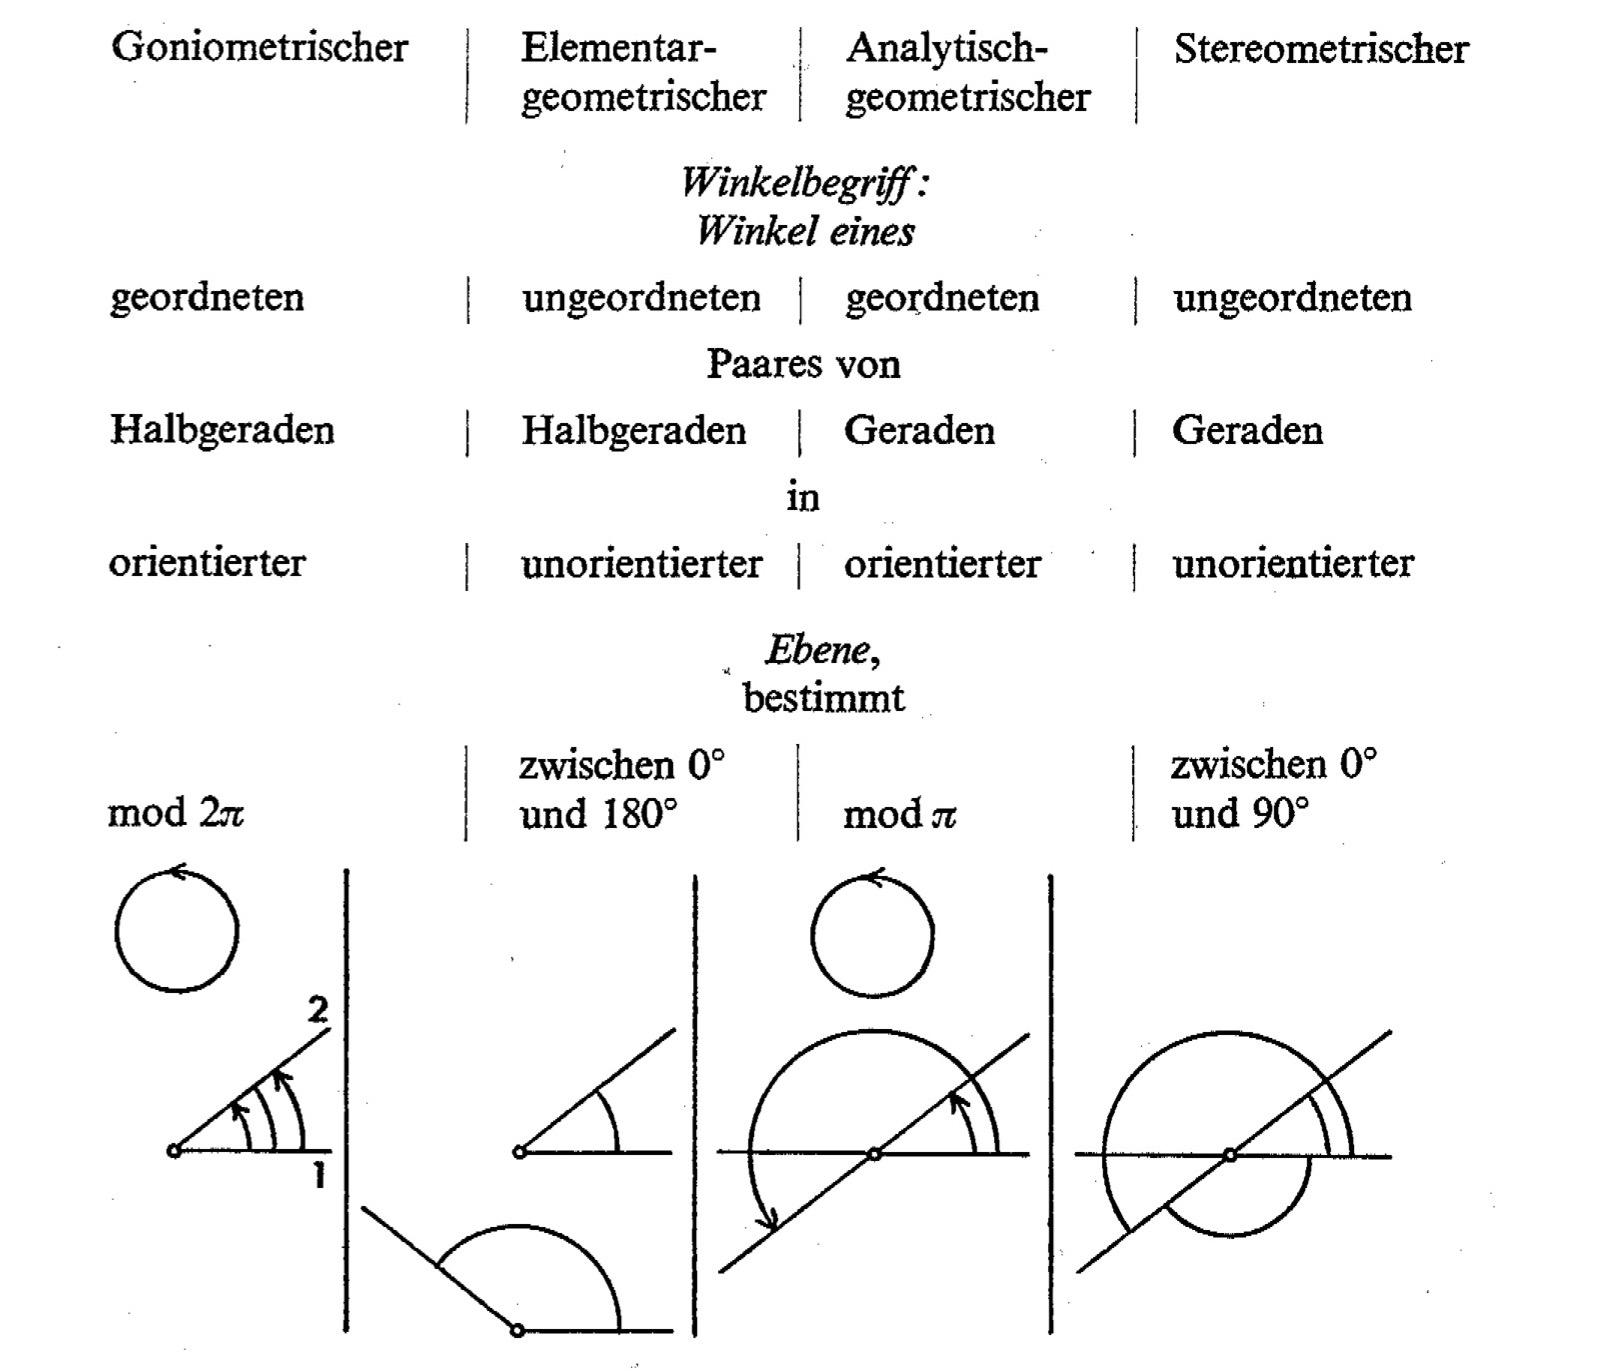
\includegraphics[width=0.75\linewidth]{pictures/1-FreudenthalWinkel} 

}

\caption{Winkelbegriffe nach Freudenthal (\citeproc{ref-Freudenthal:1973}{1973b, S. 441})}\label{fig:FreudenthalWinkel}
\end{figure}

Er diskutiert, welchen Einfluss die jeweilige Sichtweise auf dem Maßbereich hat, wie Winkel überhaupt gemessen werden können und wie mit Winkeln operiert werden kann. Was passiert denn, wenn man ein geordnetes Strahlenpaar in der orientierten Ebene spiegelt (vgl. \citeproc{ref-Freudenthal:1973}{Freudenthal, 1973b, 443~ff.})?

Wenn die Reihenfolge der Strahlen erhalten bleibt und die Winkelmessung aufgrund der Orientierung der Ebene vorgegeben ist, ändert sich damit ggf. auch das Maß des Winkels (siehe Abbildung \ref{fig:FreudenthalWinkelSpiegeln}).



\begin{figure}

{\centering 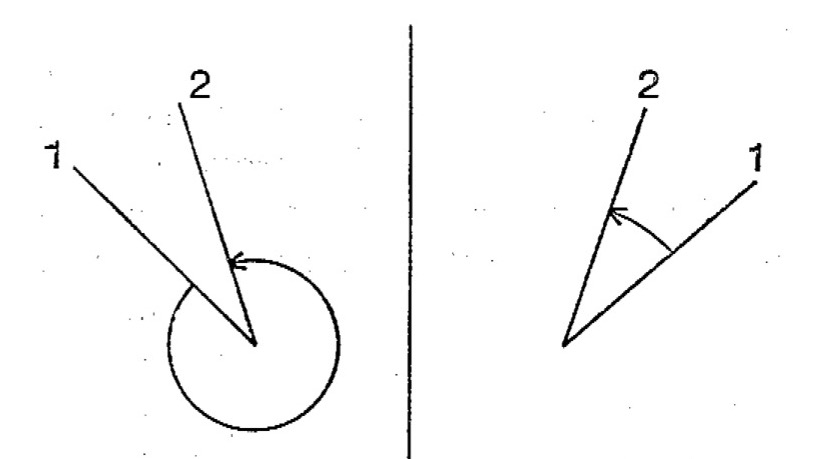
\includegraphics[width=0.5\linewidth]{pictures/1-FreudenthalWinkelSpiegeln} 

}

\caption{Spiegelung eines goniometrischen Winkels (\citeproc{ref-Freudenthal:1973}{Freudenthal, 1973b, 443})}\label{fig:FreudenthalWinkelSpiegeln}
\end{figure}

Hierzu stellt Freudenthal (\citeproc{ref-Freudenthal:1973}{1973b, 443~ff.}) weitere fachmathematische Ausführungen dar und schließt damit, dass der elementargeometrische, goniometrische und analytische Winkelbegriff aus fachlicher Sicht für den schulischen Lernpfad unentbehrlich sind (\citeproc{ref-Freudenthal:1973}{Freudenthal, 1973b, S. 449}).

Die \emph{Spezifizierung} besteht also darin, den Begriff zu schärfen und Operationen mit ihm zu beschreiben. Die \emph{Strukturierung} besteht u.~a. in der vernetzenden Analyse der verschiedenen Winkelbegriffe und der Schlussfolgerung ihrer gleichermaßen Bedeutsamkeit für den Schulunterricht.\index{Vier-Ebenen-Ansatz!formale Ebene|)}

\subsection{Semantische Ebene}\label{semantische-ebene}

Dazu,\index{Vier-Ebenen-Ansatz!semantische Ebene|(} welche Vorstellungen Schülerinnen und Schüler zum Winkelbegriff entwickeln sollen, sei u.~a. auf Krainer (\citeproc{ref-Krainer:1989}{1989}) und Mitchelmore \& White (\citeproc{ref-Mitchelmore:1998}{1998}) verwiesen. Eine grundsätzliche Schwierigkeit beim Unterrichten von Winkeln sind diverse und (scheinbar) nicht in Verbindung zu bringende Anwendungskontexte, die dennoch über denselben mathematischen Begriff beschrieben werden können. So ist das Sichtfeld eines Tieres ebenso wie die Umdrehung eines Wasserzählers über Winkel beschreibbar -- haben doch beide Situationen zunächst nichts miteinander zu tun.

Aufbauend auf den Arbeiten von Krainer (\citeproc{ref-Krainer:1989}{1989}) und Mitchelmore \& White (\citeproc{ref-Mitchelmore:1998}{1998}) können über eine Verknüpfung zur formalen Ebene mithilfe einer \emph{informationstheoretischen Winkeldefinition} (\citeproc{ref-Etzold2021}{Etzold, 2021, 39~f..}) vier Grundvorstellungen zum Winkelbegriff ausgearbeitet bzw. validiert werden:

\begin{itemize}
\tightlist
\item
  Winkel als Knick
\item
  Winkel als Feld
\item
  Winkel als Richtungsänderung
\item
  Winkel als Umdrehung
\end{itemize}

Dabei erhalten die \emph{Bestandteile} eines Winkels (Scheitelpunkt, Schenkel, ggf. Bereich zwischen den Schenkeln, Abweichungsmaß) eine besondere Bedeutung, über die sich auch eine sinnvolle Reihenfolge der Behandlung dieser Grundvorstellungen ableiten lässt. So »bietet es sich an, mit den Winkelfeldern zu beginnen. Bei diesen werden die meisten Bestandteile sichtbar (Scheitelpunkt, beide Schenkel als Begrenzungen sowie der zwischen den Schenkeln relevante Bereich) {[}\ldots{]}. Anschließend können Knicke oder Richtungsänderungen behandelt werden, woraufhin die Umdrehungen folgen.« (\citeproc{ref-Etzold2021}{Etzold, 2021, S. 60})

Die \emph{Spezifizierung} in diesem semantischen Teil ist demnach die Ausarbeitung der Grundvorstellungen. Die Begründung einer möglichen Reihenfolge kann der \emph{Strukturierung} des Lerngegenstands zugeordnet werden.\index{Vier-Ebenen-Ansatz!semantische Ebene|)}

\subsection{Konkrete Ebene}\label{konkrete-ebene}

Um\index{Vier-Ebenen-Ansatz!konkrete Ebene|(} die einzelnen Vorstellungen zu Winkeln aufzubauen, bedarf es charakteristischer Situationen, an denen der mathematische Kern der jeweiligen Vorstellung besonders gut sichtbar wird. Abbildung \ref{fig:Winkelsituationen} zeigt derartige \emph{Winkelsituationen} und die zugehörigen Grundvorstellungen (hier \emph{Winkelkontexte}).



\begin{figure}

{\centering 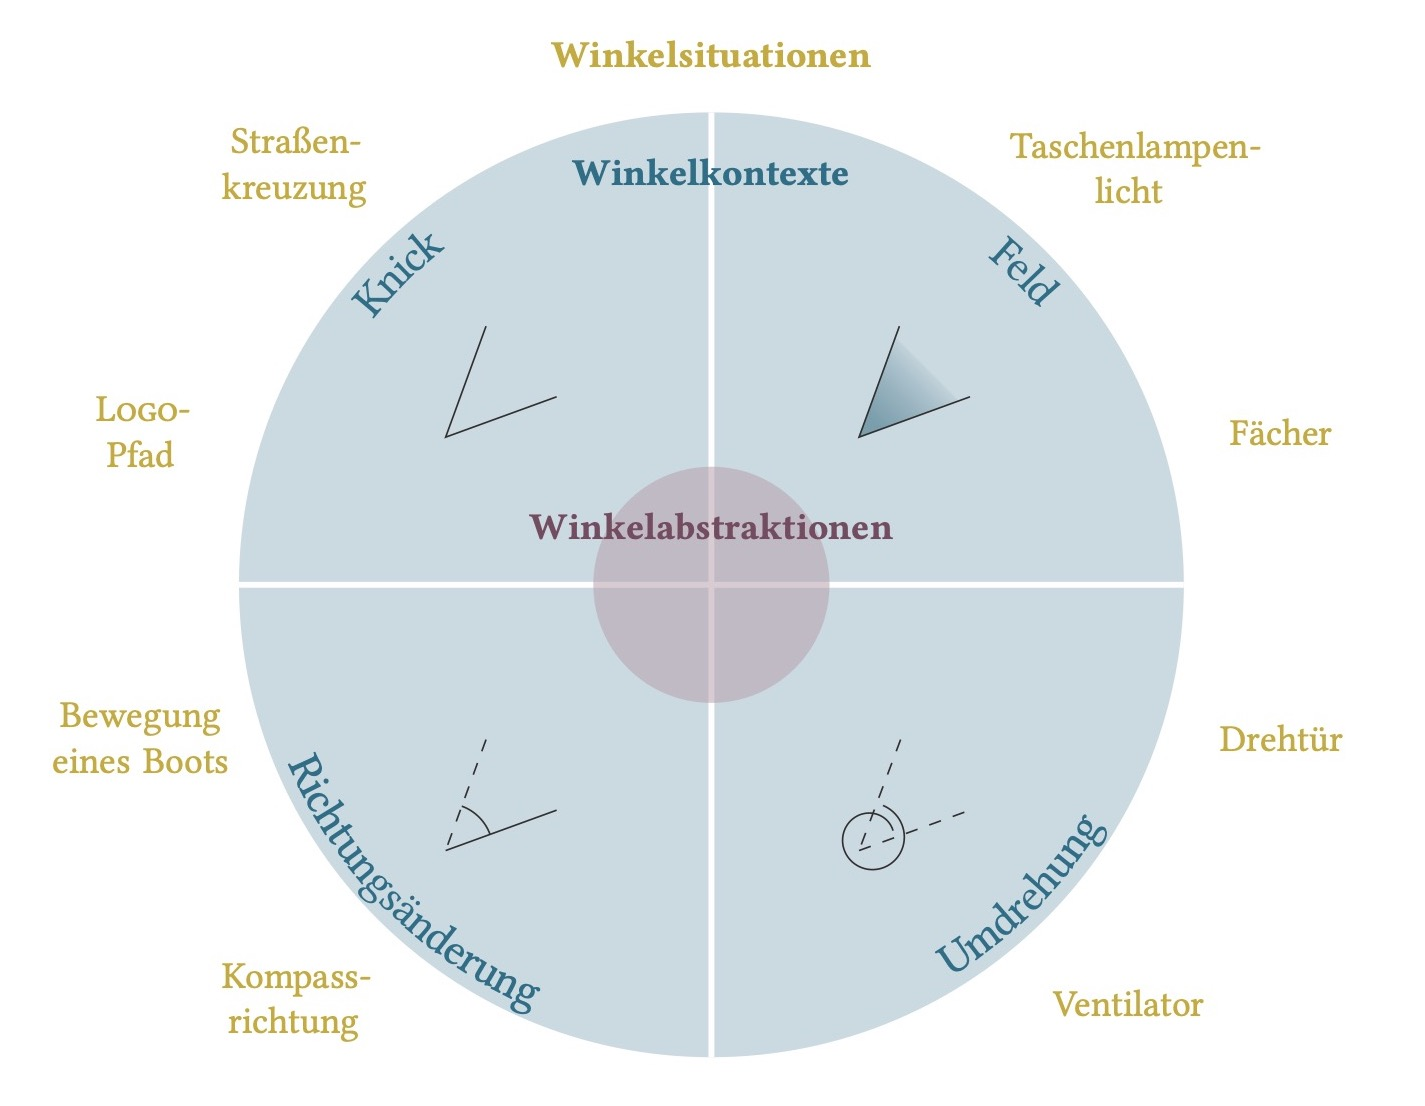
\includegraphics[width=0.75\linewidth]{pictures/1-Winkelsituationen} 

}

\caption{Winkelsituationen und -kontexte (\citeproc{ref-Etzold2021}{Etzold, 2021, S. 70})}\label{fig:Winkelsituationen}
\end{figure}

Exemplarisch für die Grundvorstellung des Winkels als Feld wird darauf aufbauend eine Lernumgebung und darin eingebettetes Unterrichtsmaterial entwickelt, mithilfe dessen die Grundvorstellung ausgebildet werden kann. An der konkreten Situation der \emph{Sichtfelder von Tieren} sollen die Schülerinnen und Schüler Handlungen ausführen, die es ihnen ermöglicht, den mathematischen Kern hinter dem konkreten Beispiel zu erkunden.

Die Schülerinnen und Schüler nutzen dazu eine App (siehe Abbildung \ref{fig:WinkelfarmApp}), in der mehrere Tiere mit ihren Sichtfeldern dargestellt werden können, und erhalten u.~a. folgende Aufgaben (vgl. \citeproc{ref-Etzold:2019Praxis4}{Etzold, 2019b, S. 8~ff.}):

\begin{enumerate}
\def\labelenumi{\arabic{enumi}.}
\tightlist
\item
  Setze das Schaf an eine Stelle, an der es von der Kuh gesehen wird, aber die Kuh selbst nicht sieht.
\item
  Setze das Schaf an eine Stelle, an der es nicht von der Kuh gesehen wird.
\item
  Das Schaf will die Kuh verwirren. Bewege es an möglichst viele Orte, an denen es von der Kuh gesehen wird.
\item
  Setze das Schaf an eine Stelle, an der es noch gerade so von der Kuh gesehen wird.
\item
  Wo muss das Schaf lang laufen, damit es die gesamte Zeit gerade so von der Kuh gesehen wird?
\end{enumerate}

An Aufgabe 5 kann z.~B. erkundet werde, dass sich das Schaf geradlinig auf der Grenze zwischen Sichtfeld und Nicht-Sichtfeld bewegen muss. In die eine Richtung ist die Bewegung beliebig fortsetzbar, in die andere durch den Kopf der Kuh begrenzt. Eine mathematische Verallgemeinerung dieser Handlung besteht dann in der Identifizierung des Schenkels (Begrenzung) als Strahl (nur in eine Richtung fortsetzbar) mit dem Scheitelpunkt (Kopf der Kuh) als \emph{Quelle} des Winkelfeldes.



\begin{figure}

{\centering 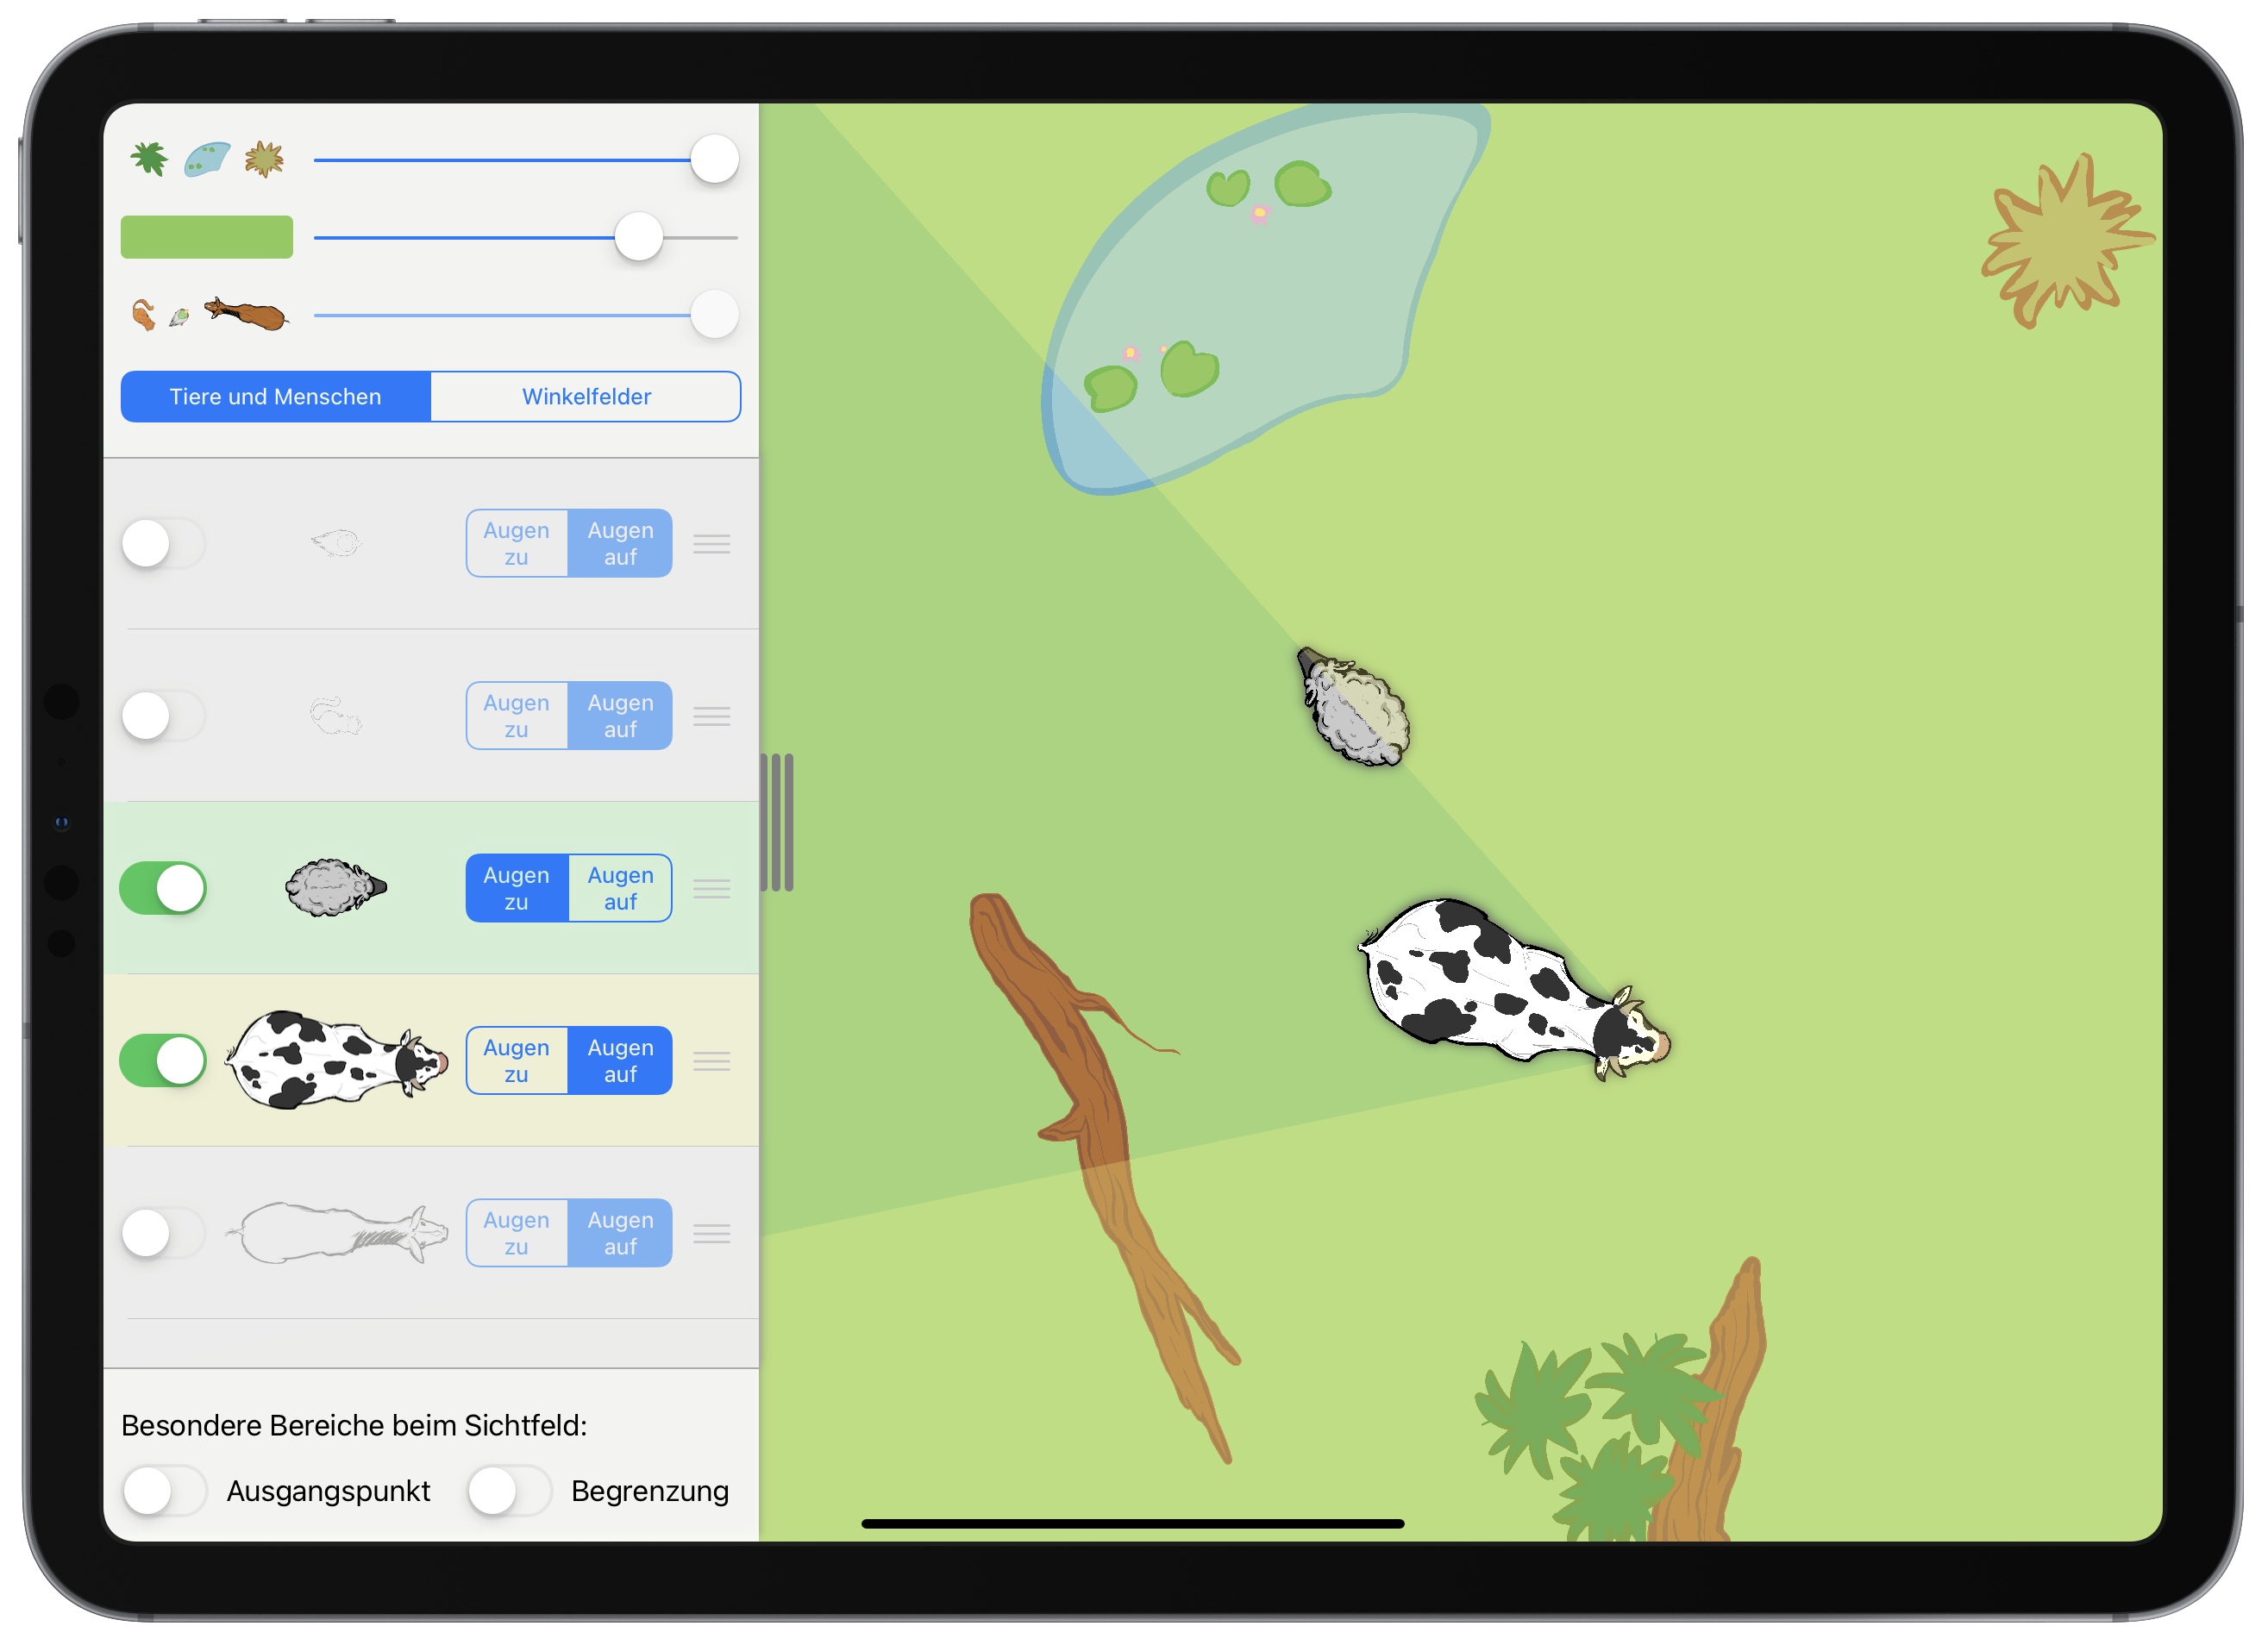
\includegraphics[width=0.75\linewidth]{pictures/1-Winkelfarm} 

}

\caption{Screenshot der App Winkel-Farm (\citeproc{ref-Etzold:2019}{Etzold, 2019a})}\label{fig:WinkelfarmApp}
\end{figure}

Als \emph{Spezifizierung} kann das Finden der Sichtfeld-Situation als charakterisches Beispiel für ein Winkelfeld angesehen werden. Die \emph{Strukturierung} führt zum dargestellten Lernpfad und den konkreten Aufgabenstellung, über die konkrete Handlungen verallgemeinert werden und damit das mathematische Verständnis aufgebaut wird.\index{Vier-Ebenen-Ansatz!konkrete Ebene|(}

\subsection{Empirische Ebene}\label{empirische-ebene}

Die\index{Vier-Ebenen-Ansatz!empirische Ebene|(} zuvor beschriebene Lernumgebung wurde in mehreren Zyklen erprobt und dabei die Qualität der Handlungen der Schülerinnen und Schüler beobachtet. Ein Ziel bestand darin, dass möglichst verallgemeinerbare Handlungen (wie oben am Beispiel des Schenkels beschrieben) durchgeführt werden.

Es wird erwartet, dass die Repräsentation eines Sichtfeldes von der Draufsicht über eine semintransparent ausgemalte Teilfläche der Ebene noch nicht bekannt ist. Um diese nachzuvollziehen und mit eigenen Erfahrungen in Bezug zu bringen, wird an den Beginn der Unterrichtsstunde ein Bild des Klassenraumes in der Draufsicht präsentiert (siehe Abbildung \ref{fig:Klassenraum}). Dann soll eine Schülerin oder ein Schüler beschreiben, was sie/er alles sieht, ohne den Kopf zu drehen. Dieser Bereich wird auf dem Bild eingezeichnet, so dass die Repräsentation des Sichtfeldes im Folgenden zur Verfügung steht.

\begin{figure}

{\centering 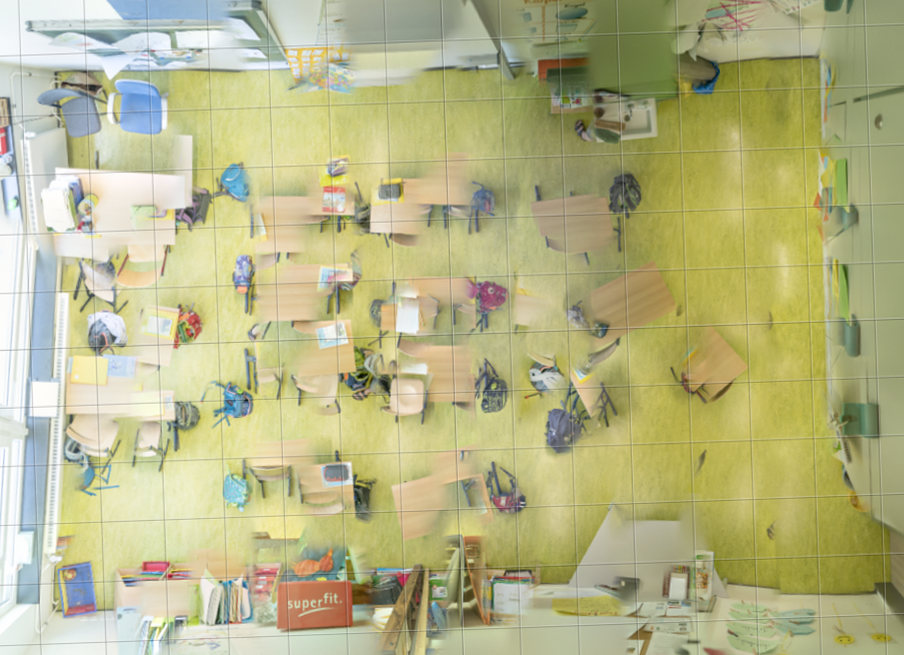
\includegraphics[width=0.75\linewidth]{pictures/1-Klassenraum} 

}

\caption{Klassenraum von oben (Foto: Christian Dohrmann)}\label{fig:Klassenraum}
\end{figure}

In der Erprobung konnte beobachtet werden, dass einige Bedienschwierigkeiten mit der Anwendung den Lernfortschritt hemmten. Dies konnte u.~a. dadurch verbessert werden, dass vor die eigentliche Erarbeitung eine freie Erkundungsphase mit der App (siehe Abbildung \ref{fig:WinkelfarmStart}) gesetzt wurde (\citeproc{ref-Etzold2021}{Etzold, 2021, S. 147, 152}). Durch spezifische Aufgabenstellungen wurden bestimmte Funktionen der App fokussiert:

\begin{figure}

{\centering 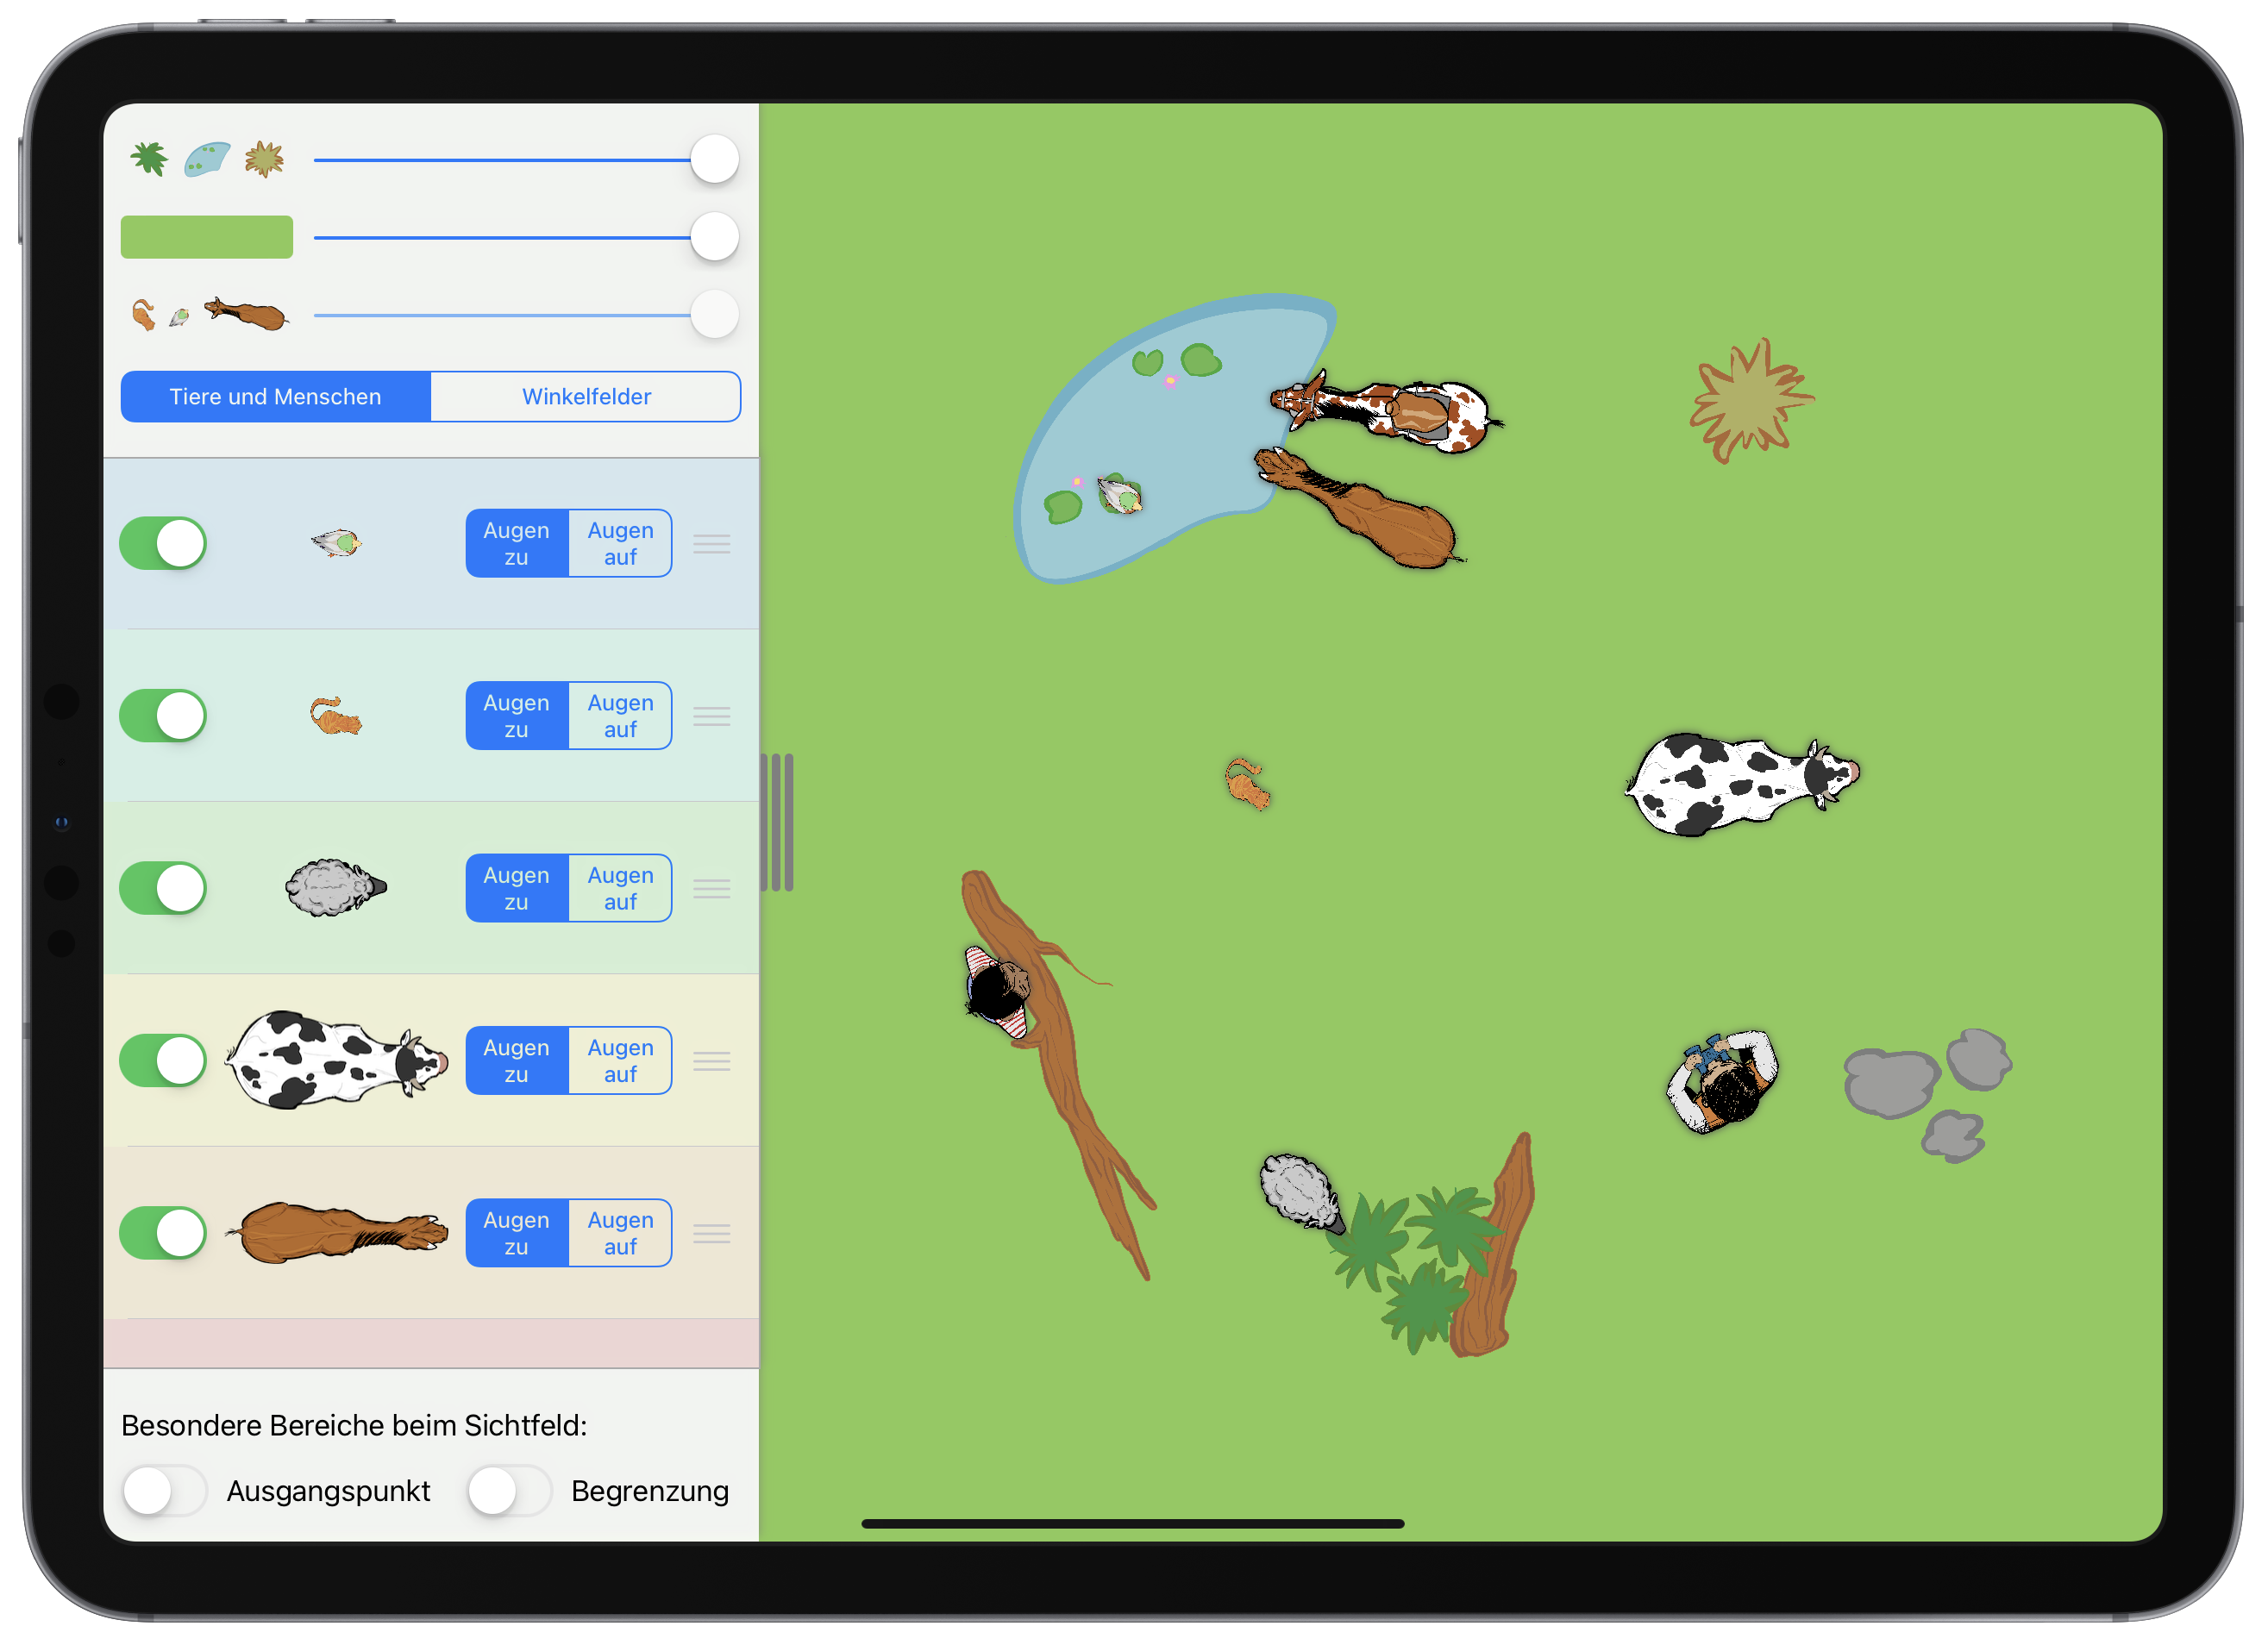
\includegraphics[width=0.75\linewidth]{pictures/1-WinkelfarmStart} 

}

\caption{Möglicher Startbildschirm für die freie Erkundungphase}\label{fig:WinkelfarmStart}
\end{figure}

\emph{»Das Pferd soll auf dem Steinpflaster stehen, die Frau soll auf dem Pferd sitzen/stehen. Das Pferd guckt in Richtung der grünen Büsche, die Frau hat die Augen zu. Gleichzeitig versteckt sich die Katze unter der Kuh.«}

Die Einführungsphase über das Klassenraumfoto folgt aus der \emph{Spezifizierung} innerhalb der empirischen Ebene. Das Hinzufügen der freien Erkundungsphase ist dagegen der \emph{Strukturierung} der Analyse zuzuordnen.\index{Winkel|)}\index{Vier-Ebenen-Ansatz!empirische Ebene|)}

\subsection{Verknüpfung der Ebenen}\label{verknuxfcpfung-der-ebenen}

An den Ausführungen ist schon sichtbar geworden, dass sich die Ebenen nicht immer trennen lassen und teilweise gegenseitig beeinflussen. Auch gehen oft Spezifizierung und Strukturierung ineinander über.

Das ist aber gar nicht schlimm, ganz im Gegenteil. Es zeigt wieder einmal, wie wichtig solch ein ganzheitlicher Ansatz ist, so dass eine stoffdidaktische Analyse aus den diversen Sichtpunkten heraus betrachtet werden sollte.

Wichtig ist v.~a., dass Sie sich als Lehrkraft stets darüber im Klaren sind, dass für eine stoffdidaktische Analyse verschiedene Perspektiven verfolgt werden müssen. Sehen Sie den Vier-Ebenen-Ansatz daher auch als Kontrollinstrument, ob Sie an alles gedacht haben, wenn Sie einen Lerngegenstand intensiv analysieren.

\section{Zum Nachbereiten}\label{vier-ebenen-nachbereitung}

\begin{enumerate}
\def\labelenumi{\arabic{enumi}.}
\tightlist
\item
  Lesen Sie den Artikel von Hußmann \& Prediger (\citeproc{ref-Hussmann:2016}{2016}) zum Vier-Ebenen-Ansatz.
\item
  Reflektieren Sie Ihre bisherige Fach- und Fachdidaktikausbildung in Mathematik dahingehend, welche der aufgeworfenen Fragen Sie zu konkreten Themenbereichen (nicht) beantworten könnten.
\end{enumerate}

\chapter{(Hoch-)Schulmathematik strukturieren}\label{hoch-schulmathematik-strukturieren}

\begin{quote}
\textbf{Ziele}

\begin{itemize}
\tightlist
\item
  Sie erkennen den Nutzen der Hochschulmathematik bei der Entscheidungsfindung zur Spezifizierung und Strukturierung der Schulmathematik auf der formalen Ebene des Vier-Ebenen-Ansatzes.
\item
  Sie kennen geeignete Quellen zur Beantwortung der Fragen auf der formalen Ebene des Vier-Ebenen-Ansatz\\
\item
  Sie kennen verschiedene Möglichkeiten, Mathematik zu strukturieren.\\
\item
  Sie können beschreiben, woher die verschiedenen Strukturierungsmöglichkeiten kommen.
\end{itemize}

\textbf{Material}

\begin{itemize}
\tightlist
\item
  Folien zum Kapitel 2 (\href{files/Stoffdidaktik2024-02-HochSchulmathematikStrukturieren.pdf}{pdf}, \href{files/Stoffdidaktik2024-02-HochSchulmathematikStrukturieren.key}{Keynote})
\end{itemize}
\end{quote}

\section{Doppelte Diskontinuität}\label{doppelte-diskontinuituxe4t}

Auf der \textcolor{formalColor}{formalen Ebene} des Vier-Ebenene-Ansatzes soll der zu betrachtende Lerngegenstand fachmathematisch untersucht werden, um eine erste Auswahl (\emph{Spezifizierung}) und Anordnung (\emph{Strukturierung}) der Lerninhalte zu ermöglichen. Dies ruft natürlich -- auch für Lerngegenstände der Grundschulmathematik -- danach, die im Studium erworbenen hochschulmathematischen Erkenntnisse zu nutzen. Dieser Ruf wird jedoch (scheinbar!) geschmälert durch eine offensichtliche Ungleichheit zwischen Schulmathematik und Hochschulmathematik. Felix Klein beschreibt dieses Phänomen, das sich insbesondere auf die Ausbildung von Lehrkräften auswirkt, bereits im Übergang vom 19. zum 20. Jahrhunderts als \textbf{\emph{doppelte Diskontinuität}}: »Der junge Student sieht sich am Beginn seines Studiums vor Probleme gestellt, die ihn in keinem Punkte mehr an die Dinge erinnern, mit denen er sich auf der Schule beschäftigt hat; natürlich vergißt er daher alle diese Sachen rasch und gründlich. Tritt er aber nach Absolvierung des Studiums ins Lehramt über, so soll er plötzlich eben diese herkömmliche Elementarmathematik schulmäßig unterrichten; da er diese Aufgabe kaum selbständig mit seiner Hochschulmathematik in Zusammenhang bringen kann, so wird er in den meisten Fällen recht bald die althergebrachte Unterrichtstradition aufnehmen, und das Hochschulstudium bleibt ihm nur eine mehr oder minder angenehme Erinnerung, die auf seinen Unterricht keinen Einfluß hat.« (\citeproc{ref-Klein1967}{Klein, 1967, S. 1})\footnote{Es handelt sich hier um den Nachdruck eines Werke, dessen erste Auflage 1908 erschien.}

Einen Ausweg, dieser doppelten Diskontinität zu entgehen, sah Klein in einer \textbf{\emph{Elementarmathematik vom höheren Standpunkte aus}} (\citeproc{ref-Klein1925}{Klein, 1925}, \citeproc{ref-Klein1955}{1955}, \citeproc{ref-Klein1967}{1967}). Dabei verfolgt er »das Ziel, im Anschluss an umfassende hochschulmathematische Erfahrungen die Schulmathematik in den erworbenen Wissenskanon fachlich einzubetten« (\citeproc{ref-Danckwerts2013}{Danckwerts, 2013, S. 78}).

Diesen Gedanken fortsetzend kann man auch »gleich am Anfang des Studiums direkt und explizit an die schulmathematischen Vorerfahrungen an{[}knüpfen{]}, bleibt inhaltlich bei diesen und arbeitet einen höheren Standpunkt heraus, der auf die vertiefte Auseinandersetzung mit der Oberstufenmathematik zielt und prinzipiell mit den bis dahin erworbenen (elementar-)mathematischen Mitteln auskommt.« (\citeproc{ref-Danckwerts2013}{Danckwerts, 2013, S. 78}) Eine solche Entwicklung hat das Projekt \emph{Mathematik Neu Denken} verfolgt, das gut 100 Jahre nach Kleins Publikationen die Lehramtsausbildung im Fach Mathematik weiterentwickeln wollte (\citeproc{ref-Beutelspacher2012}{Beutelspacher et al., 2012}). Entwickelt wird daraus eine \textbf{\emph{Schulmathematik vom höheren Standpunkt}}, die auf eine fachliche und verstehensorientierte Durchdringung der Schulmathematik zielt, »ohne im vollen Umfang auf das Instrumentarium der kanonischen {[}\ldots{]} {[}Hochschulmathematik{]} zurückgreifen zu müssen« (\citeproc{ref-Danckwerts2013}{Danckwerts, 2013, S. 87}).

Im Rahmen der Stoffdidaktik-Veranstaltung sollen beide Ansätze aufgegriffen und an konkreten Beispielen versucht werden, die Fragen der \textcolor{formalColor}{formalen Ebene} zu beantworten. Als bedeutsames Bindeglied zwischen Schul- und Hochschulmathematik stellen sich dabei fundamentale Ideen heraus, die auch schon auf die \textcolor{semanticColor}{semantische Ebene} des Vier-Ebenen-Ansatzes zielen -- siehe dazu Abschnitt \ref{fundamentale-ideen}.

\section{Geeignete Quellen}\label{geeignete-quellen}

\begin{itemize}
\item
  Neben den Werken von Felix Klein zu Beginn des 20. Jahrhunderts (\citeproc{ref-Klein1925}{Klein, 1925}, \citeproc{ref-Klein1955}{1955}, \citeproc{ref-Klein1967}{1967}) und aktuellen Ansätzen zum Umgang mit der doppelten Diskontinuität in der Lehramtsausbildung (\citeproc{ref-Ableitinger2013}{Ableitinger et al., 2013}; \citeproc{ref-Beutelspacher2012}{Beutelspacher et al., 2012}) liefern die in den 1970er Jahren von Hans Freudenthal verfassten Werke zur \emph{Mathematik als pädagogische Aufgabe} (\citeproc{ref-Freudenthal1973a}{Freudenthal, 1973c}, \citeproc{ref-Freudenthal:1973}{1973b}; englischsprachig auch digital verfügbar über \citeproc{ref-Freudenthal1973c}{Freudenthal, 1973a}) Ansätze, Schul- und Hochschulmathematik miteinander in Bezug zu bringen.
\item
  Ebenfalls hilfreich sind größere Nachschlagewerke zur Mathematik, bspw. die \emph{Kleine Enzyklopädie Mathematik} (\citeproc{ref-Gellert1986}{Gellert et al., 1986}).
\item
  Nicht zu unterschätzen für die fachmathematische Auseinandersetzung sind auch fachdidaktische Quellen, insbesondere zur \textbf{Didaktik der Sachgebiete}. Als digital verfügbare Quellen seien zu erwähnen:

  \begin{itemize}
  \tightlist
  \item
    \emph{Didaktik der Algebra: nach der Vorlage von Hans-Joachim Vollrath} (\citeproc{ref-Weigand2022}{Weigand et al., 2022})
  \item
    \emph{Didaktik der Geometrie für die Sekundarstufe I} (\citeproc{ref-Weigand2018}{Weigand et al., 2018})
  \item
    \emph{Didaktik der Analysis. Aspekte und Grundvorstellungen zentraler Begriffe} (\citeproc{ref-Greefrath2016}{Greefrath et al., 2016})
  \item
    \emph{Didaktik der Stochastik in der Sekundarstufe I} (\citeproc{ref-Kruger2015}{Krüger et al., 2015})
  \item
    \emph{Didaktik der Analytischen Geometrie und Linearen Algebra: Algebraisch verstehen -- Geometrisch veranschaulichen und anwenden} (\citeproc{ref-Henn2015}{Henn \& Filler, 2015})
  \item
    \emph{Mathematikunterricht in der Sekundarstufe II. Band 1: Fachdidaktische Grundfragen, Didaktik der Analysis} (\citeproc{ref-Tietze:2000a}{Tietze et al., 2000a})
  \item
    \emph{Mathematikunterricht in der Sekundarstufe II. Band 2: Didaktik der Analytischen Geometrie und Linearen Algebra} (\citeproc{ref-Tietze:2000}{Tietze et al., 2000b})
  \item
    \emph{Mathematikunterricht in der Sekundarstufe II. Band 3: Didaktik der Stochastik} (\citeproc{ref-Tietze:2002}{Tietze et al., 2002})
  \end{itemize}
\item
  Ebenfalls hilfreich für die fachliche Spezifizierung und Strukturierung kann die Darstellung der Fachinhalte in \textbf{Schulbüchern} sein. Hier bietet sich eine vergleichende Analyse mehrerer Schulbücher, auch unterschiedlicher Bundesländer, an.
\item
  Nur gering geeignet für die Spezifizierung und Strukturierung sind die Bildungsstandstandards und Rahmenlehrpläne. Sie bieten -- entsprechend ihrer Funktion -- bereits eine Auswahl der zu unterrichtenden Inhalte und schränken damit die fachdidaktische Diskussion diesbezüglich ein.
\end{itemize}

\section{Strukturierungsmöglichkeiten}\label{strukturierungsmuxf6glichkeiten}

Mathematik kann auf verschiedene Weisen strukturiert werden. Manche Strukturierungsmöglichkeiten orientieren sich stärker an der Fachwissenschaft (z.~B. \emph{Sachgebiete}), andere an der Bedeutung der Fachinhalte für die mathematische Kultur an sich (z.~B. \emph{Fundamentale Ideen}). Im Folgenden werden vier Strukturierungsmöglichkeiten vorgestellt.

\subsection{Sachgebiete}\label{sachgebiete}

Für die Fachwissenschaft Mathematik haben sich historisch verschiedene Unterdisziplinen entwickelt, die als Sachgebiete der Mathematik bezeichnet werden können. Schulrelevante Gebiete sind hierbei:

\begin{itemize}
\tightlist
\item
  Arithemtik
\item
  Algebra
\item
  Geometrie
\item
  Analysis
\item
  Stochastik
\item
  Lineare Algebra / Analytische Geometrie
\end{itemize}

Auch heute bilden sich diese und weitere Sachgebiete (z.~B. Numerik) in den Strukturen von universitären Lehrveranstaltungen, Forschungsrichtungen und nicht zuletzt der Strukturierung einzelner Lehrpläne der Schulen ab.

Für eine Vertiefung mit der Didaktik der Sachgebiete eignen sich u.~a. die in Abschnitt \ref{geeignete-quellen} dargestellten Quellen. Weiterhin werden Sie im Masterstudium im Modul \emph{Ausgewählte Themen der Mathematikdidaktik}\footnote{siehe Modulbeschreibung zum Modul \href{https://puls.uni-potsdam.de/qisserver/rds?state=verpublish&status=init&vmfile=no&moduleCall=modulansicht&publishConfFile=modulverwaltung&publishSubDir=up/modulbearbeiter&&modul.modul_id=3186&menuid=&topitem=Modulbeschreibung&subitem=}{MAT-LS-D3 bei PULS}} die Möglichkeit haben, sich mit der Didaktik einzelner Sachgebiete näher auseinanderzusetzen.

\subsection{Leitideen}\label{leitideen}

Die Strukturierung mathematischer Inhalte in Leitideen ist seit Anfang der 2000er Jahre im deutschen Bildungswesen etabliert, als die KMK\footnote{Mehr zur Kultusministerkonferenz (KMK) und ihrer eigentlichen Bezeichnungen siehe Wikipedia (\citeproc{ref-dewiki:228417777}{2022b}).} \textbf{Bildungsstandards} für den Mittleren Schulabschluss (2004), den Primarbereich (2005) und später auch die Allgemeine Hochschulreife (2012) herausgebracht hat. Darauf aufbauend wurden in den meisten Bundesländern die Lehrpläne angepasst.
Zwischenzeitlich wurden die Bildungsstandards für den Primarbereich sowie den Ersten und Mittleren Schulabschluss überarbeitet, für die gymnasiale Oberstufe gelten während der gerade laufenden Überarbeitung noch die von 2012. (\citeproc{ref-KMK:2012}{Sekretariat der Ständigen Konferenz der Kultusminister der Länder in der Bundesrepublik Deutschland, 2012}, \citeproc{ref-SekretariatderStandigenKonferenzderKultusministerderLanderinderBundesrepublikDeutschland2022a}{2022b}, \citeproc{ref-SekretariatderStandigenKonferenzderKultusministerderLanderinderBundesrepublikDeutschland2022}{2022a}).
In Brandenburg spiegeln sich die Bildungsstandards in den \textbf{Rahmenlehrplänen} für die Jahrgangsstufen 1~--~10 und die Gymnasiale Oberstufe wider (\citeproc{ref-MinisteriumfurBildungJugendundSportdesLandesBrandenburg2022}{Ministerium für Bildung, Jugend und Sport des Landes Brandenburg, 2022}, \citeproc{ref-MinisteriumfuerBildungJugendundSportdesLandesBrandenburg2023}{2023}).

Im Laufe der letzten 20 Jahre haben sich für die Leitideen teils verschiedene Bezeichnungen ergeben. In den aktuellen Bildungsstandards des Ersten und Mittleren Schulabschlusses (\citeproc{ref-SekretariatderStandigenKonferenzderKultusministerderLanderinderBundesrepublikDeutschland2022}{Sekretariat der Ständigen Konferenz der Kultusminister der Länder in der Bundesrepublik Deutschland, 2022a}) werden verwendet:

\begin{itemize}
\tightlist
\item
  Leitidee Zahl und Operation
\item
  Leitidee Größen und Messen
\item
  Leitidee Strukturen und funktionaler Zusammenhang
\item
  Leitidee Raum und Form
\item
  Leitidee Daten und Zufall
\end{itemize}

Die Leitidee Zahl und Operation beispielweise »umfasst sinntragende Vorstellungen und Darstellungen von Zahlen und Operationen sowie die Nutzung von Rechengesetzen und Kontrollverfahren. Dazu gehören die sachgerechte Nutzung von Prozent- und Zinsrechnung ebenso wie kombinatorische Überlegungen und Verfahren, denen Algorithmen zu Grunde liegen.« (\citeproc{ref-SekretariatderStandigenKonferenzderKultusministerderLanderinderBundesrepublikDeutschland2022}{Sekretariat der Ständigen Konferenz der Kultusminister der Länder in der Bundesrepublik Deutschland, 2022a, S. 15}). Weiterhin werden diese Kompetenzen an spezifischen Fachinhalten konkretisiert, etwa: »Die Schülerinnen und Schüler {[}\ldots{]} • untersuchen Zahlen nach ihren Faktoren, in einfachen Fällen ohne digitale Mathematikwerkzeuge, • stellen Zahlen der Situation angemessen dar, z.B. unter anderem in Zehnerpotenzschreibweise, • rechnen mit natürlichen, ganzen und rationalen Zahlen, die im täglichen Leben vorkommen, sowohl zur Kontrolle als auch im Kopf und erklären die Bedeutung der Rechenoperationen {[}\ldots{]}« (\citeproc{ref-SekretariatderStandigenKonferenzderKultusministerderLanderinderBundesrepublikDeutschland2022}{Sekretariat der Ständigen Konferenz der Kultusminister der Länder in der Bundesrepublik Deutschland, 2022a, S. 15})

Die Leitideen werden in den Bildungsstandards als \textbf{inhaltsbezogene Kompetenzen} beschrieben, die mit Abschluss des ersten bzw. mittleren Schulabschlusses zu erreichen sind. Es handelt sich dabei um \textbf{Regelstandards}, also Kompetenzen, die »Schülerinnen und Schüler im Durchschnitt in einem Fach erreichen sollen« (\citeproc{ref-SekretariatderStandigenKonferenzderKultusministerderLanderinderBundesrepublikDeutschland2022}{Sekretariat der Ständigen Konferenz der Kultusminister der Länder in der Bundesrepublik Deutschland, 2022a, S. 2}). Diese sind abzugrenzen gegenüber \textbf{Basiskompetenzen} als »mathematisch zentrale, instrumentell bedeutsame und geradezu grundlegende Konzepte und Verfahren, die für die mathematische Kompetenzentwicklung unverzichtbar sind« (vgl. \url{https://pikas-mi.dzlm.de/node/92}). Für Basiskompetenzen gibt es derzeit in Deutschland keine politischen Dokumente wie Rahmenlehrpläne oder Bildungsstandards.

\subsection{Arten mathematischen Wissens}\label{arten-mathematischen-wissens}

Eine weitere Strukturierung mathematischen Wissens kann darin bestehen, den Blick darauf zu lenken, wie dieses Wissen angeeignet wird. So können ähnliche Aneigungsprozesse Motivation bieten, das Wissen entsprechend zu strukturieren und dies dann für die Gestaltung von Lehr-Lern-Prozessen nutzbar zu machen. Etabliert hat sich hierfür eine Unterscheidung in drei Arten mathematischen Wissens (vgl. \citeproc{ref-Vollrath2012}{Vollrath \& Roth, 2012, S. 45}~f.):

\begin{itemize}
\item
  \textbf{Begriffe.} Diese bilden das Grundgerüst der Mathematik und belegen Objekte gleicher Eigenschaft mit einem gemeinsamen Bezeichner. Neben der Begriffsfestlegung, i.~d.~R. über eine Definition, ist der Einsatz geeignter Beispiele und Gegenbeispiele essentiell beim Aufbau eines Begriffsverständnisses.
\item
  \textbf{Zusammenhänge} Diese beschreiben Eigenschaften von Begriffen und ihre Beziehungen zueinander. Klassischerweise gehören hierzu mathematische Sätze inkl. ihrer Beweise, aber auch präformale Begründungen. Bei Vollrath \& Roth (\citeproc{ref-Vollrath2012}{2012, 45~f.}) wird statt von \emph{Zusammenhängen} von \emph{Sachverhalten} gesprochen, ältere Quellen beziehen sich auch nur auf \emph{Sätze}.
\item
  \textbf{Verfahren.} Diese bestimmen, wie bestimmte Aufgaben zu lösen sind, z. B. schriftliche Rechenverfahren, Lösungsverfahren von Gleichungen und Gleichungssystemen.
\end{itemize}

Einige Autoren zählen zu den Verfahren auch heuristische Strategien zum Problemlösen oder die Anwendung des Permanenzprinzips (vgl. \citeproc{ref-Steinhofel1988}{Steinhöfel et al., 1988, S. 23}). Vollrath \& Roth (\citeproc{ref-Vollrath2012}{2012, S. 46}~ff.) ergänzen dagegen die drei Wissensarten noch:

\begin{itemize}
\tightlist
\item
  \textbf{Metamathematisches Wissen.} Darunter ist zu verstehen, \emph{wie} Mathematik betrieben wird, also bspw. welche Möglichkeiten es gibt, ein mathematisches Problem zu lösen oder eine Sachsituation mathematisch zu modellieren.
\end{itemize}

In den nächsten Kapiteln wird näher darauf eingegangen, wie Lernprozesse bei der Ausbildung der jeweiligen Wissensarten gestaltet werden können.

\subsection{Fundamentale Ideen}\label{fundamentale-ideen}

\subsubsection{Begriffsklärung}\label{fundamentale-ideen-begriffsklaerung}

Die Entwicklung Fundamentaler Ideen beruft sich auf Bruners Annahme, dass »jedes Kind {[}\ldots{]} auf jeder Entwicklungsstufe jeder Lehrgegenstand in einer intellektuell ehrlichen Form erfolgreich gelehrt werden« kann (vgl. \citeproc{ref-Bruner:1976}{Bruner, 1976, S. 77}). Voraussetzung dafür ist, dass die \emph{Struktur} eines Inhaltsbereichs in einer Art und Weise präsentiert wird, dass sie dem Kind zugänglich wird. Diese \emph{hinter den Dingen} liegende Struktur hebt sich vom konkreten Inhaltsbereich ab, ist allgemeinerer Natur und kann daher über \emph{Fundamentale Ideen} beschrieben werden.

Ziel der Orientierung des Unterrichtens an Fundamentalen Ideen besteht v.~a. darin, die (oftmals) isolierten Stoffelemente einzuordnen und in einem größeren Ganzen zu sehen. Im Umkehrschluss heißt dies aber auch, dass die Auswahl des konkreten Stoffes daran orientiert sein muss, wie dieser dazu beitragen kann, den dahinter liegenden mathematischen Kern und die zugehörigen Fundamentalen Ideen zu vertreten.

Die dazu seit den 1960er Jahren in Gang gesetzte Forschung führte zu vielfältigen Vorschlägen Fundamentaler Ideen der Mathematik -- jedoch bisher nicht zu einem allgemeingültigen Katalog. Dieser Vielfalt in den Formulierungen und Kategorisierungen kann begegnet werden, indem Fundamentale Ideen über Eigenschaften charakterisiert werden. Schwill (\citeproc{ref-Schwill:1994}{1994}) schlägt hierzu vor.

»Eine \textbf{Fundamentale Idee}\index{Fundamentale Idee|textbf} bzgl. eines Gegenstandsbereichs (Wissenschaft, Teilgebiet) ist ein \textbf{Denk-, Handlungs-, Beschreibungs- oder Erklärungsschema}, das

\begin{enumerate}
\def\labelenumi{\arabic{enumi}.}
\tightlist
\item
  in verschiedenen Gebieten des Bereichs vielfältig anwendbar oder erkennbar ist (\textbf{Horizontalkriterium}),\index{Fundamentale Idee!Horizontalkriterium|textbf}
\item
  auf jedem intellektuellen Niveau aufgezeigt und vermittelt werden kann (\textbf{Vertikalkriterium}),\index{Fundamentale Idee!Vertikalkriterium|textbf}
\item
  in der historischen Entwicklung des Bereichs deutlich wahrnehmbar ist und längerfristig relevant bleibt (\textbf{Zeitkriterium}),\index{Fundamentale Idee!Zeitkriterium|textbf}
\item
  einen Bezug zu Sprache und Denken des Alltags und der Lebenswelt besitzt (\textbf{Sinnkriterium}).\index{Fundamentale Idee!Sinnkriterium|textbf}«
\end{enumerate}

Fundamentale Ideen haben zwar ihren Ursprung in der Fachstruktur, aber sie »sind nicht Elemente der Wissenschaft an sich, sondern Produkte unseres Verstandes, die wir der Wissenschaft aufprägen. Folglich können sie nur relativ zum Menschen objektiviert werden« (\citeproc{ref-Schubert:2011}{Schubert \& Schwill, 2011, S. 62}).

\begin{quote}
\textbf{Überblick zur historischen Entwicklung Fundamentaler Ideen}

\begin{itemize}
\tightlist
\item
  von der Bank (\citeproc{ref-Bank:2016}{2016, 37~ff.}): \emph{Fundamentale Ideen der Mathematik: Weiterentwicklung einer Theorie zu deren unterrichtspraktischer Nutzung}
\end{itemize}
\end{quote}

Für Ihre stoffdidaktische Analyse können Fundamentale Ideen insbesondere hilfreich für die \textbf{Dekonstruktion} des Fachwissens und anschließende \textbf{Rekonstruktion} des Schulwissens sein.

Wenn sie also beispielsweise eine stoffdidaktische Analyse zur Flächeninhaltsberechnung durchführen, setzen Sie sich mit der Fundamentalen Idee des \emph{Messens}\index{Messen} auseinander. Dabei verstehen Sie Messvorgänge als Vergleiche zu einem Standardmaß (z.~B. Kästchen auszählen), erkennen Zerlegungs- und Ergänzungsgleichheit als notwendige Prinzipien zur präziseren Beschreibung, sehen Dreiecke als bedeutsame Basisfiguren für Flächeninhaltsberechnungen an und haben den Blick für die Integralrechnung als verallgemeinerbare Methode zur Flächeninhaltsbestimmung krummliniger Figuren (vgl. \citeproc{ref-Vohns:2000}{Vohns, 2000, 98~ff.}). Sie \emph{dekonstruieren} (zerlegen) damit Ihr eigenes mathematisches Fachwissen.

Nun sind Sie in der Lage, das Wissen zur Flächeninhaltsberechnung für Schülerinnen und Schüler neu aufzubauen, also zu \emph{rekonstruieren} und (unter Hinzunahme der Betrachtung von Grundvorstellungen und den restlichen Ebenen des Vier-Ebenen-Ansatzes) einen Lernpfad zu entwickeln. Im Zusammenhang mit der Integralrechnung kann dies z.~B. heißen, dass Sie parallel zum Bilden von Ober- und Untersummen noch einmal eine krummlinig begrenzte Fläche durch Kästchen auszählen lassen -- ggf. mit unterschiedlicher Feinheit und einer Abschätzung nach oben und nach unten. Die Fundamentalen Ideen haben für Sie damit auch eine \emph{ordnende Funktion} des Unterrichtsstoffes.

\begin{figure}

{\centering 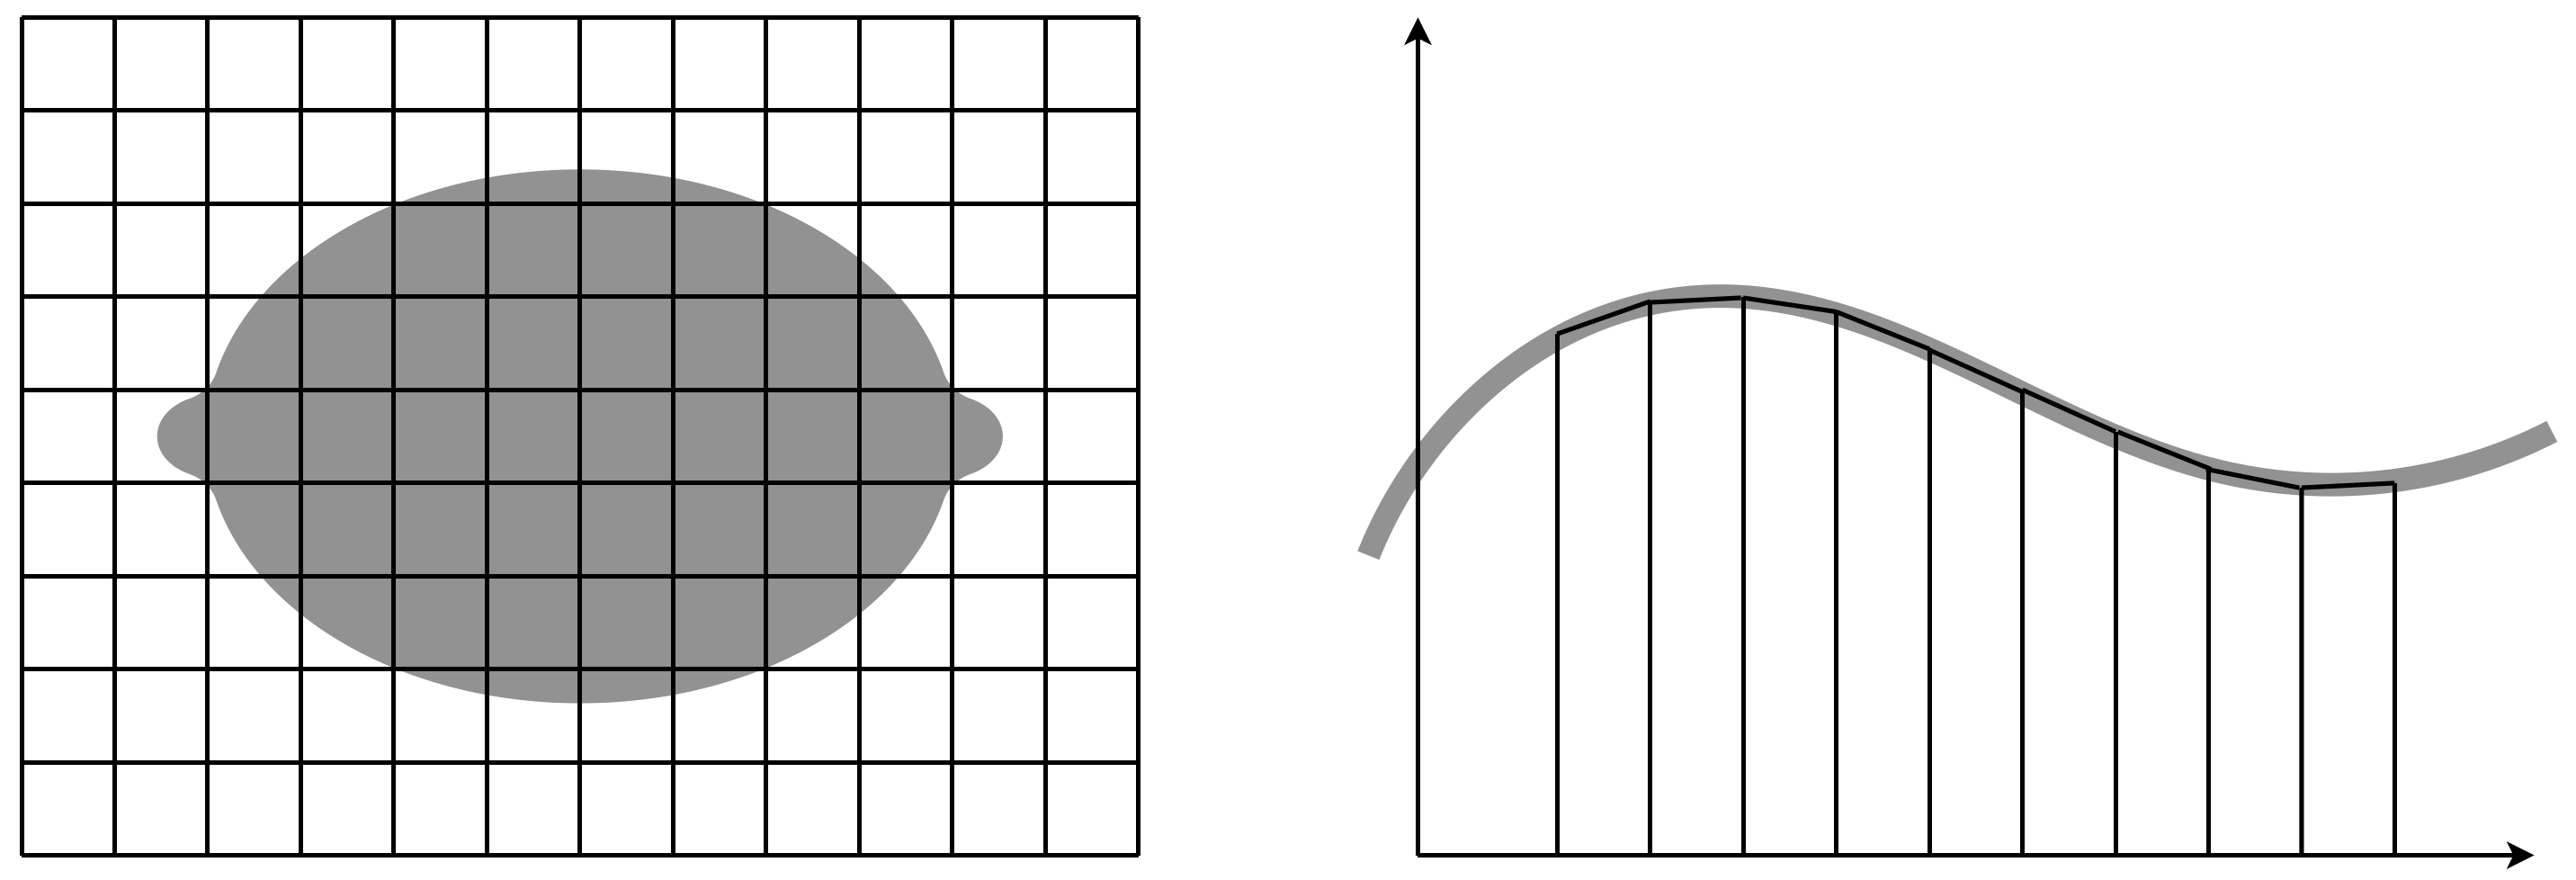
\includegraphics[width=0.75\linewidth]{pictures/3-Flaeche} 

}

\caption{Flächeninhaltsbestimmung}\label{fig:Flaeche}
\end{figure}

\subsubsection{Auswahl Fundamentaler Ideen}\label{auswahl-fundamentaler-ideen}

Das Fehlen eines allgemeingültigen Katalogs sollte nicht davon abhalten, bestehende Auflistungen und Strukturierungen Fundamentaler Ideen zu betrachten. von der Bank (\citeproc{ref-vonderBank:2013}{2013, S. 103}) und Lambert (\citeproc{ref-Lambert:2012}{2012}) diskutieren eine Kategorisierung Fundamentaler Ideen in drei Bereiche:

\begin{itemize}
\item
  \textbf{Inhaltsideen} beziehen sich auf konkrete Inhaltsbereiche der Mathematik, die die Kriterien Fundamentaler Ideen erfüllen können. Nicht ganz zufällig spiegeln diese sich in den Leitideen der Bildungsstandards wider (siehe Abschnitt \ref{leitideen}).
\item
  \textbf{Schnittstellenideen} haben die Eigenschaft, dass durch sie die »Mathe(matik) wirkt« und »auch für andere Fächer in ihrer je spezifischen Weise relevant sind« (\citeproc{ref-Lambert:2012}{Lambert, 2012}). Damit korrelieren sie mit den prozessbezogenen Kompetenzen der Bildungsstandards.
\item
  \textbf{Tätigkeitsideen} beziehen sich insbesondere auf innermathematische Tätigkeiten, die sich über verschiedene Inhaltsbereiche hinweg zeigen. Lambert (\citeproc{ref-Lambert:2012}{2012}) betont, dass es diese (über die Bildungsstandards hinaus) ebenfalls zu beachten gilt, wenn man einen reichhaltigen Mathematikunterricht bewirken möchte.
\end{itemize}

Beispiele derartiger Tätigkeitsideen sind:

\begin{itemize}
\tightlist
\item
  Approximierung
\item
  Optimierung
\item
  Linearität/Linearisierung
\item
  Symmetrie
\item
  Invarianz
\item
  Rekursion
\item
  Vernetzung
\item
  Ordnen
\item
  Strukturierung
\item
  Formalisierung
\item
  Exaktifizierung
\item
  Verallgemeinern
\item
  Idealisieren
\end{itemize}

Im Rahmen des Projektmoduls \emph{Erweitertes Fachwissen für den schulischen Kontext in Mathematik}\footnote{siehe Modulbeschreibung zum Modul \href{https://puls.uni-potsdam.de/qisserver/rds?state=verpublish&status=init&vmfile=no&moduleCall=modulansicht&publishConfFile=modulverwaltung&publishSubDir=up/modulbearbeiter&&modul.modul_id=3156&menuid=&topitem=Modulbeschreibung&subitem=}{MAT-LS-7 bei PULS}} werden Sie insbesondere Bezüge zwischen Schul- und Hochschulmathematik auf Basis Fundamentaler Ideen herstellen, wofür die Inhalts- und Tätigkeitsideen von hoher Relevanz sind.

\subsubsection{Beispiel Linearität}\label{beispiel-linearitaet}

\paragraph*{Horizontal- und Vertikalkriterium}\label{horizontal--und-vertikalkriterium}
\addcontentsline{toc}{paragraph}{Horizontal- und Vertikalkriterium}

Linearität\index{Linearität|(}\index{Fundamentale Idee!Horizontalkriterium|(}\index{Fundamentale Idee!Vertikalkriterium|(} ist ein wesentliches Konzept über die gesamte Schullaufbahn hinweg (und darüber hinaus). Dies spiegelt sich in vielfältigen Themenbereichen wider, die sowohl die Breite (\emph{Horizontalkriterium}) als auch Tiefe (\emph{Vertikalkriterium}) von Linearität und (später) auch Linearisierung zeigen. Dieser Abschnitt orientiert sich an den Darstellungen von Danckwerts (\citeproc{ref-Danckwerts:1988}{1988}).

\begin{itemize}
\tightlist
\item
  Linearität als Phänomen tritt schon im Geometrieunterricht der Grundschule mit \textbf{Geraden} als essentielle geometrische Objekte auf. In der euklidischen Geometrie sind Geraden neben Punkten die Basisobjekte eines axiomatischen Aufbaus.
\item
  Das \textbf{Distributivgesetz} \(a\cdot (b+c) = a\cdot b + a\cdot c\), das ebenfalls bereits in der Grundschule behandelt wird, beschreibt einen linearen Vorgang und bietet die Grundlage für die halbschriftliche Multiplikation. Über die Schulmathematik hinaus dient es z.~B. als eines der Vektorraumaxiome (Skalarmultiplikation).
\item
  Das Bestimmen eines \textbf{Rechteckflächeninhalts} ist ein linearer Vorgang: Ein Rechteck, das doppelt so breit ist, hat (bei gleicher Höhe) einen doppelt so großen Flächeninhalt. Betrachtet man diese Eigenschaft nicht als Phänomen, sondern als Forderung an eine Flächeninhaltsformel, so kann aus den Bedingungen \(A(a_1+a_2,b) = A(a_1,b) + A(a_2,b)\) und \(A(a,b_1+b_2) = A(a,b_1)+A(a,b_2)\) sowie der Stetigkeit in \(\mathbb{R}^+\) die Formel \(A(a,b) = a\cdot b\) abgeleitet werden.
\item
  Lineare Zuordnungen der Art \(f(x+y) = f(x)+f(y)\) werden zu Beginn der Sekundarstufe I als \textbf{proportionale Zuordnungen} behandelt. Dies wird fortgeführt bei \textbf{linearen Funktionen} der Art \(f(x) = mx+n\), in der Fachmathematik als affin-lineare Abbildungen bezeichnet.
\item
  \textbf{Lineare Gleichungen und Gleichungssysteme} sind ebenfalls bedeutsamer Bestandteil des Mathematikunterrichts. Überhaupt baut die gesamte \textbf{Lineare Algebra} auf lineare und affin-lineare Abbildungen auf.
\item
  Die \textbf{Strahlensätze} beschreiben ebenfalls ein lineares Verhalten: Geradenabschnitte in \(c\)-facher Entfernung sind \(c\) mal so lang.
\end{itemize}

\begin{figure}

{\centering 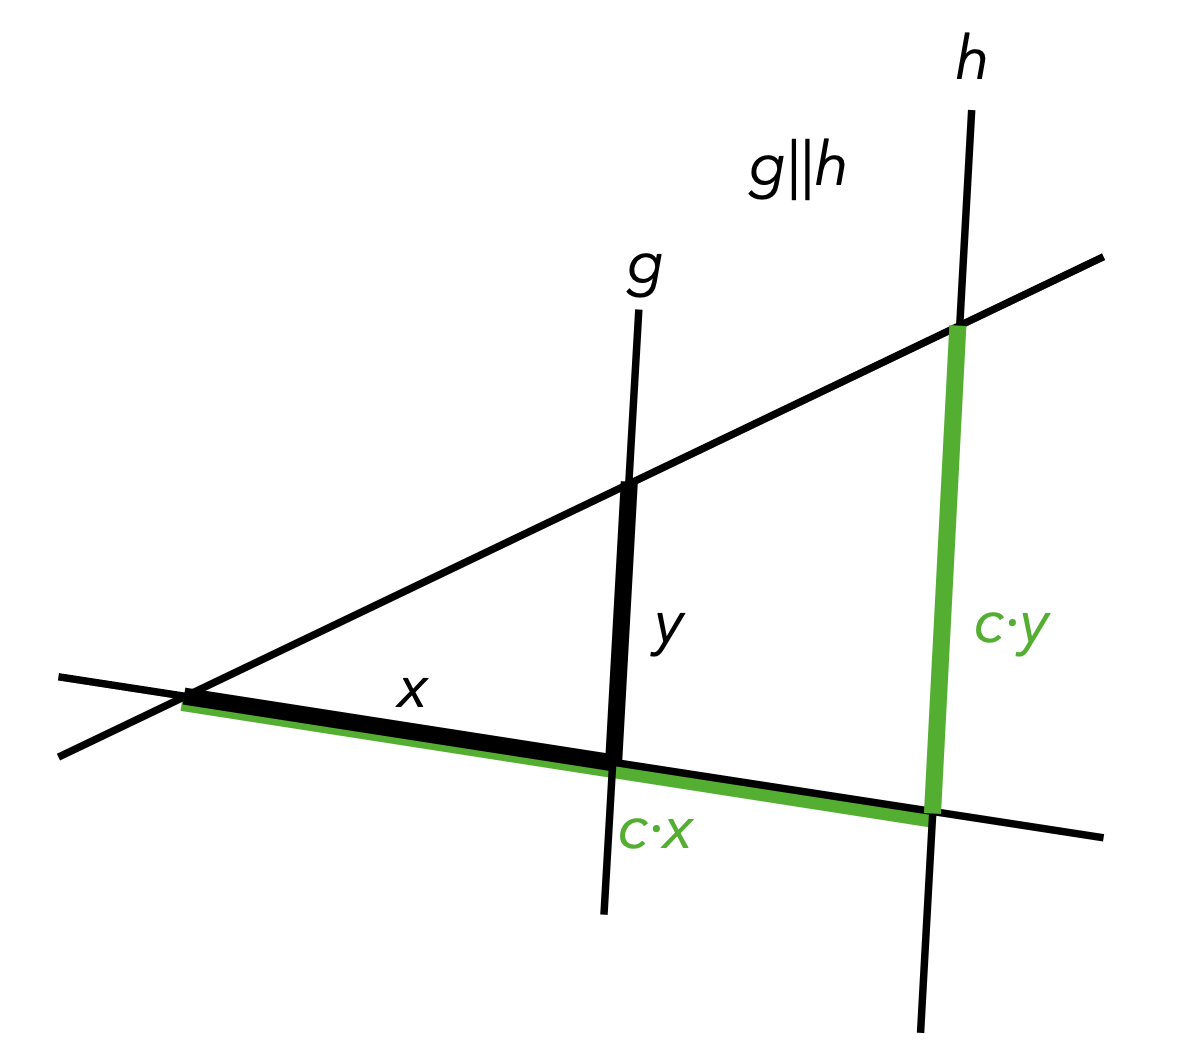
\includegraphics[width=0.5\linewidth]{pictures/3-Strahlensatz} 

}

\caption{Strahlensatzfigur}\label{fig:Strahlensatz}
\end{figure}

\begin{itemize}
\tightlist
\item
  Beim \textbf{Ableitungsbegriff} ist eine wesentliche Vorstellung, dass die Funktion in der Umgebung der zu betrachtenden Stelle linearisiert wird. Insbesondere bei höherdimensionalen Funktionen wird der Linearisierungsansatz weiterverfolgt. Die ebenfalls vorherrschende Tangentenvorstellung ist auf mehr als drei Dimensionen nicht mehr anschaulich übertragbar -- der Linearisierungsansatz weist hier aufgrund seiner algebraischen Beschreibung die bessere Verallgemeinerbarkeit auf.
\item
  Eng an den Linearisierungsansatz angelehnt ist die \textbf{lineare Approximation} von Funktionen (z.~B. \(\sin(x)\approx x\) für \(x\approx 0\)). Die führt sich in der Hochschulmathematik fort, beispielsweise bei Taylor-Reihen.
\item
  Das Bedürfnis der Linearisierung, insbesondere aus der Physik heraus, zeigt sich auch bei der Nutzung \textbf{spezifisch skalierter Diagrammachsen}, z.~B. von Logarithmuspapier. Wegen der Äquivalenz von \(y = c\cdot a^x\) und \(\ln y = (\ln a )\cdot x + \ln c\) lassen sich beliebige Exponentialfunktionen auf Logarithmuspapier als lineare Funktionen darstellen.
\item
  Verschiedene Näherungsverfahren, wie das \textbf{Newton-Verfahren}, bedienen sich ebenfalls der Linearisierung.
\end{itemize}

An dieser Stelle sei darauf hingewiesen, dass Linearität derart fundamental ist, dass selbst nicht-lineare Zusammenhänge häufig fälschlicherweise als linear angenommen werden. Dies zeigt sich zum Beispiel an den Fehlannahmen \((x+y)^2 \overset{?!}{=} x^2+y^2\), \(\sqrt{x+y} \overset{?!}{=} \sqrt{x}+\sqrt{y}\) oder \(\sin(x+y) \overset{?!}{=} \sin(x)+\sin(y)\). Derartige Fehler können Sie als Lehrkraft besser einordnen (und korrigieren), wenn Sie sich der Fundamentalen Idee \emph{Linearität} (die hier eben \emph{nicht} gilt) bewusst sind. Insbesondere spricht dies auch für ein Explizitmachen der Fundamentalen Idee Ihren Schülerinnen und Schülern gegenüber, so dass Sie derartigen Fehlern nicht nur mit Gegenbeispielen entgegen treten können, sondern auch eine strukturelle Einordnung sichtbar machen können.

Gerade wegen der genannten Fehlannahmen und der für die Schülerinnen und Schüler i.~d.~R. nicht in Zusammenhang gebrachten Dualität aus \emph{geradlinig} und \emph{additiv und homogen} sehen Tietze et al. (\citeproc{ref-Tietze:2002}{2002, S. 39}) die Linearität dagegen nicht als eine im Mathematikunterricht etablierte Fundamentale Idee, »die die Schüler erkennen und die ihr Denken ordnet und anregt«.\index{Fundamentale Idee!Horizontalkriterium|)}\index{Fundamentale Idee!Vertikalkriterium|)}

\paragraph*{Zeit- und Sinnkriterium}\label{zeit--und-sinnkriterium}
\addcontentsline{toc}{paragraph}{Zeit- und Sinnkriterium}

Linearität\index{Fundamentale Idee!Zeitkriterium|(}\index{Fundamentale Idee!Sinnkriterium|(} zeigt sich auch in der historischen Entwicklung der Mathematik als eine prägende Leitlinie, womit sie das \emph{Zeitkriterium} Fundamentaler Ideen erfüllt. In der Linearen Algebra sei beispielsweise das Lösen linearer Gleichungssysteme im 18. Jahrhundert bis hin zum Gauß-Algorithmus im 19. Jahrhundert oder die Darstellung linearer Vorgänge mit Matrizen im 17./18. Jahrhundert erwähnt (vgl. \citeproc{ref-Tietze:2000}{Tietze et al., 2000b, 73~ff.}). In der Analysis spiegelt sich die Linearität bzw. Linearisierung in der gesamten Differenzialrechnung wider, von der Interpolation nach der Jahrtausendwende über Taylors \emph{Linear perspective} von 1715 (vgl. \citeproc{ref-Bruckler:2018}{Brückler, 2018, 39,119}) bis in die Gegenwart der linearen Modellierung nichtlinearer Zusammenhänge.

\begin{quote}
\textbf{Historische Originalausgabe}

Taylor (\citeproc{ref-Taylor:1715}{1715}): \emph{Linear perspective}
\end{quote}

Auch Alltagssituationen bzw. die Alltagssprache ist von Linearität geprägt. Beispielsweise treten proportionale Zuordnungen unmittelbar beim Einkaufen auf, wenn Waren abgewogen und der Preis bestimmt wird. Auch reale Messvorgänge, wie z.~B. die Geschwindigkeitsmessung, beziehen sich in der Regel auf die Messung von (sehr kurzen) Zeitintervallen, in denen ein lineares Verhalten angenommen wird. Das \emph{Sinnkriterium} zeigt sich aber auch in Begriffen wie \emph{lineares Fernsehen} oder \emph{lineare Erzählungen}. Dies ist zwar keine mathematische Linearität im Sinne der Formel \(f(x+y) = f(x) +f(y)\), aber der Begriff findet in einer verwandten Bedeutung in der Alltagssprache Verwendung.\index{Linearität|)}\index{Fundamentale Idee!Zeitkriterium|)}\index{Fundamentale Idee!Sinnkriterium|)}

\subsubsection{Gegenbeispiele}\label{gegenbeispiele}

Zur Verständnisförderung sollen noch ein paar Gegenbeispiele für Fundamentale Ideen angebracht werden.

\begin{itemize}
\tightlist
\item
  Das bereits erwähnte \textbf{Distributivgesetz} an sich ist zwar elementar, aber ihm fehlt die Weite, womit es nicht das Horizontalkriterium erfüllt. Die \emph{Linearität} als dahinterliegende Idee ist dagegen weit genug (vgl. ähnliche Argumentation zum \textbf{Kommutativgesetz} und der dahinterliegenden Idee der \emph{Invarianz} bei \citeproc{ref-Schubert:2011}{Schubert \& Schwill, 2011, S. 63}).
\item
  Der \textbf{Umkehrfunktion} fehlt das Sinnkriterium, da dieser Begriff in der Lebenswelt außerhab der Mathematik kaum von Relevanz ist. Dahinter liegt vielmehr die Idee der \emph{Reversibilität} als »Umkehrbarkeit von Operationen mit Wiederherstellung des Ausgangszustandes« (\citeproc{ref-Schubert:2011}{Schubert \& Schwill, 2011, S. 63}).
\end{itemize}

\section{Beispiel Negative Zahlen}\label{beispiel-negative-zahlen}

Am Beispiel der negativen Zahlen soll dargestellt werden, wie eine Sichtweise vom höheren Standpunkt auf die in der Schule relevante Behandlung dieses Lerngegenstands zur Spezifizierung und Strukturierung helfen kann. Dabei beinhalten die negativen Zahlen sowohl die ganzen Zahlen als auch die rationalen Zahlen.

\subsection{Natürliche Zahlen}\label{natuxfcrliche-zahlen}

Fachmathematisch können die ganzen Zahlen aus den natürlichen Zahlen generiert werden. Hierzu sollen zunächst die natürlichen Zahlen selbst fachmathematisch eingeordnet werden. Im Prinzip bestehen zwei Sichtweisen, nämlich die Einführung über die \textbf{Peano-Axiome} sowie die Betrachtung \textbf{gleichmächtiger Mengen}.

Aus den Peano-Axiomen (\citeproc{ref-WikiPeano}{Wikipedia, 2021}) folgt zunächst die Existenz einer Reihenfolge von Zahlen (also Nachfolger der \(0\)), die dann mit \(1\), \(2\), \(3\) usw. bezeichnet werden können.\footnote{Ab 10 wird bei der Bezeichnung jedoch das Stellenwertsystem genutzt -- das geht schon weiter als hier zulässig.} Diese Bezeichnung erlaubt jedoch noch keinerlei Berechnungen, nicht einmal eine Ordnungsrelation ist vorhanden. Es kann also (noch) nicht gesagt werden, dass \(3\) größer ist als \(1\). Vielmehr lässt sich die Situation eher mit einem Alphabet vergleichen\footnote{Ein wesentlicher Unterschied dieses Vergleiches ist, dass das Alphabet endlich ist, die Menge der natürlichen Zahlen jedoch nicht.}, bei dem auch nicht C größer als A ist.

Für eine Ordnungsrelation bedarf es zunächst der Definition der Addition über \(n+0 := n\) und \(n+k' := (n+k)'\) für alle \(n,k\in\mathbb{N}\) mit der (aus den Peano-Axiomen existierenden) Nachfolgerbildung \('\). So gilt etwa mit \(1:=0'\): \({\color{blue} 1}+{\color{red} 1} = {\color{blue} 1}+{\color{red} {0'}} = ({\color{blue} 1}+{\color{red} 0}){\color{red} '} = 1{\color{red} '} =: 2\). So kann nun induktiv jede höhere Additionsaufgabe generiert werden. Darauf aufbauend kann die Ordnungsrelation \(n<m\) über die Existenz eines \(k\in\mathbb{N}\backslash\{0\}\) mit \(m = n+k\) definiert werden. Die Subtraktion \(m-n = k\) ist nun wiederum über die Umkehroperation \(n+k = m\) definierbar, sofern \(m\geq n\).

Die Gleichmächtigkeit (z.~B. endlicher) Mengen \(M\) und \(N\) wird über die Existenz einer Bijektion zwischen diesen beiden Mengen definiert, siehe Abbildung \ref{fig:Bijektion}.

\begin{figure}

{\centering 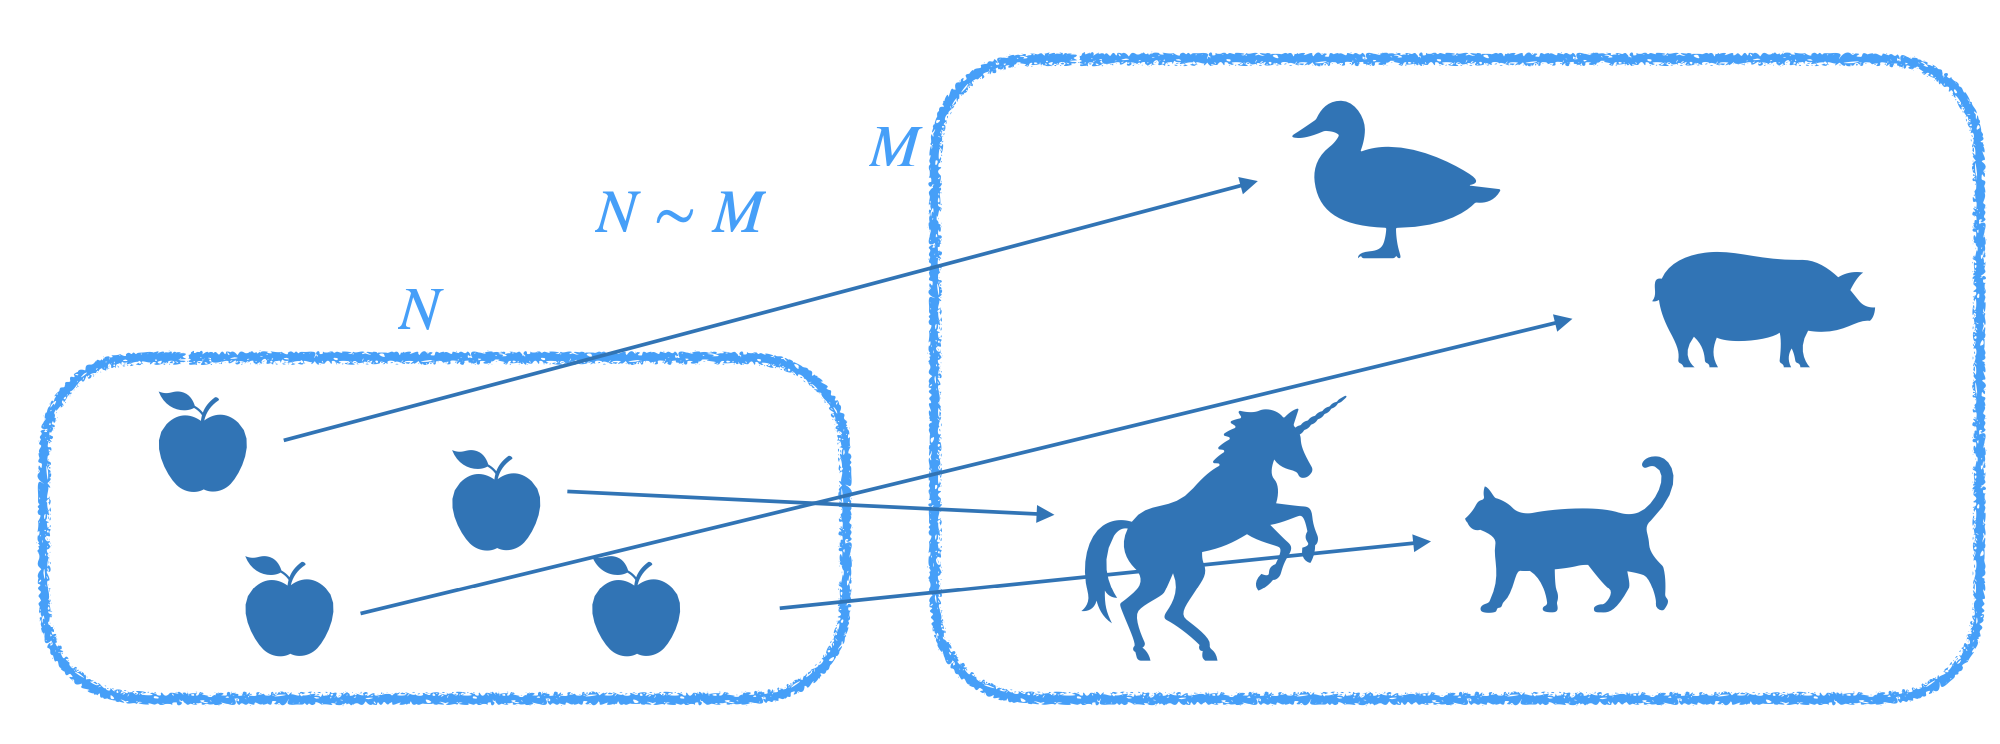
\includegraphics[width=0.75\linewidth]{pictures/2-Bijektion} 

}

\caption{Gleichmächtigkeit von Mengen}\label{fig:Bijektion}
\end{figure}

Diese Relation ist eine Äquivalenzrelation, also symmetrisch, reflexiv und transitiv. Damit können Äquivalenzklassen gebildet werden, die die Mächtigkeit der Menge angeben. \(4\) ist dann der Bezeichner für die Äquivalenzklasse von vierelementigen Mengen. Die Addition \(n+k\) entspricht dann der Mächtigkeit der Vereinigungsmenge von Mengen mit den Mächtigkeiten \(n\) und \(k\), vgl. Abbildung \ref{fig:Vereinigung}.

\begin{figure}

{\centering 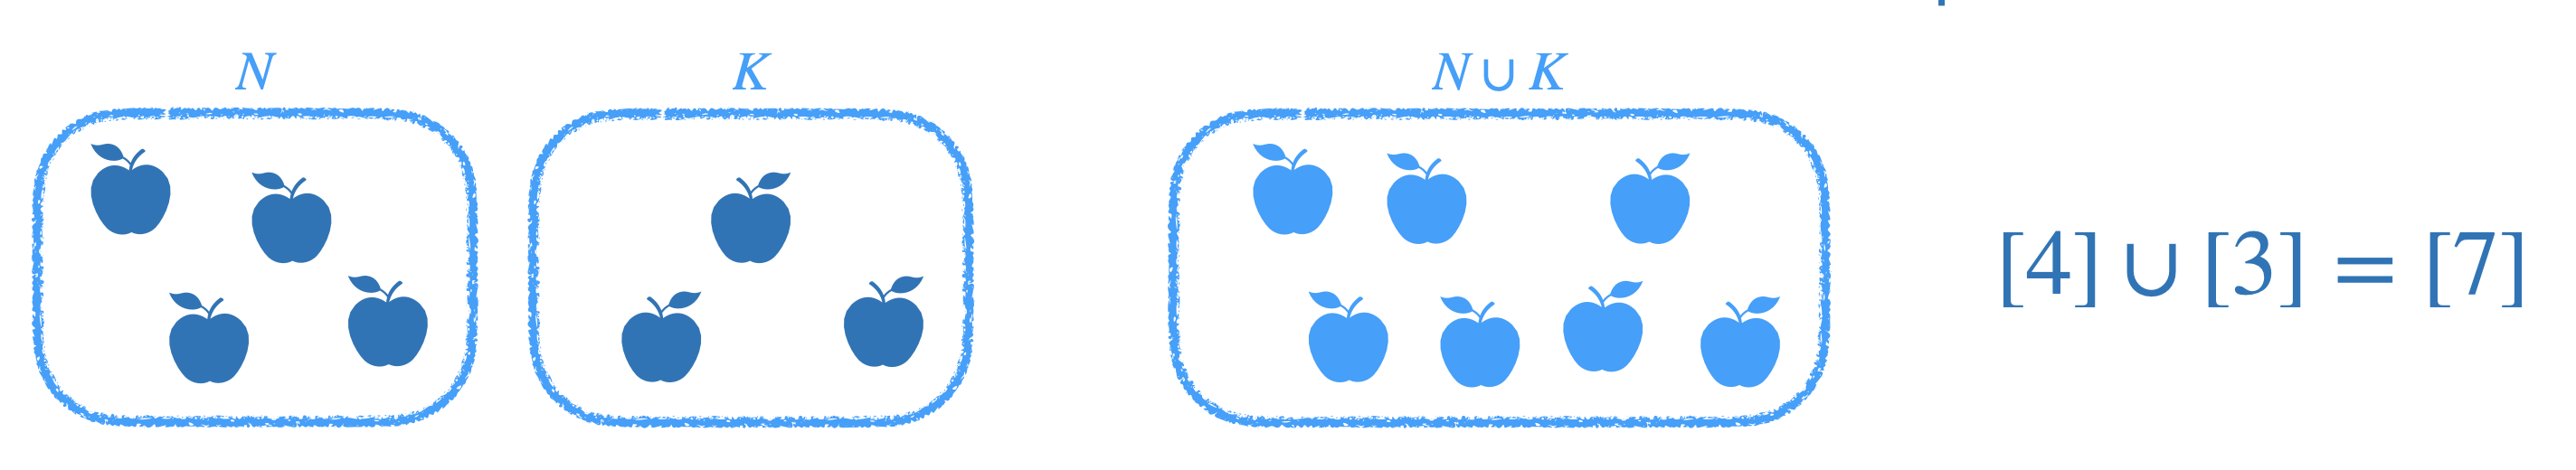
\includegraphics[width=0.9\linewidth]{pictures/2-Vereinigung} 

}

\caption{Additionsergebnis als Äquivalenzklasse der Vereinigungsmenge}\label{fig:Vereinigung}
\end{figure}

\subsection{Ganze Zahlen}\label{ganze-zahlen}

Da innerhalb der natürlichen Zahlen noch nicht beliebig subtrahiert werden darf, stehen auch keine negativen Zahlen als Ergebnisse zur Verfügung. Um dennoch das Ergebnis bspw. der Aufgabe \(2-7\) »definieren« zu können, bietet sich erneut eine \textbf{Äquivalenzrelation} über die »Differenzengleichheit« an. Konkret lässt sich für \(k,l,m,n\in\mathbb{N}\) sagen:
\((k,l)\sim (m,n):\Leftrightarrow k+n=l+m\)
Das heißt z.~B., dass die Zahlenpaare \((2,7)\), \((0,5)\) und \((4,9)\) in Relation zueinander stehen, weil sie dieselbe »Differenz« haben (obwohl es die Differenz formal noch nicht gibt). Dies ermöglicht nun die Einführung des Bezeichners \(-5\) für die Äquivalenzklasse \([(0,5)]\).

Das Vorgehen ist \emph{verträglich} mit den bisherigen Regeln in \(\mathbb{N}\), d.~h. es führt nicht zu Widersprüchen, wenn etwa das Zahlenpaar \((7,4)\) betrachtet wird mit dem Repräsentanten-Bezeichner \(3\). Die Menge aller Äquivalenzklassen (bzw. deren Kurzbezeichner) ist nun \(\mathbb{Z}\).

Die Addition und Subtraktion zweier Zahlenpaare sind nun definierbar:

\begin{align}
(k, l) + (m, n) := (k + m, l + n)\\
(k, l) − (m, n) := (k, l) + (n, m)
\end{align}

Als Alternative bietet sich ein \textbf{axiomatisches Vorgehen} an, also dass die ganzen Zahlen mit der Addition als abelsche Gruppe definiert werden -- bedeutsam ist hier insbesondere die Existenz eines Inversen zu jeder Zahl.

\subsubsection{Permanenzprinzip und Permanenzreihen}\label{permanenzprinzip-und-permanenzreihen}

Wie bereits erwähnt, führen die neu eingeführte Addition und Subtraktion in \(\mathbb{Z}\) nicht zu Konflikten mit den bisherigen analogen Operationen in \(\mathbb{N}\). Dies wird über das \textbf{\emph{Permanenzprinzip}} gefordert, nach dem neue Theorien (z.~B. das Rechnen mit negativen Zahlen) soweit wie möglich verträglich sein müssen mit bisherigen Theorien (z.~B. das Rechnen mit positiven Zahlen).

Sichtbar gemacht werden kann dieses Prinzip über \textbf{\emph{Permanenzreihen}}. Dies ist insbesondere dann hilfreich, wenn für bestimmte Rechenoperationen keine geeigneten realen Veranschaulichungen existieren. Ein typisches Beispiel hierfür ist die Multiplikation zweier negativer Zahlen. Kann die Multiplikation einer natürlichen Zahl (erster Summand) mit einer negativen Zahl (zweiter Summand) außermathematisch noch als mehrfache Verschuldung aufgefasst und die Vertauschung von erstem und zweitem Summanden über das Kommutativgesetz innermathematisch erklärt werden, bietet die Multiplikation zweier negativer Zahlen keine so naheliegende Interpretation. Abbildung \ref{fig:Permanenz} stellt eine Permanenzreihe dar, anhand derer die Rechnung \((-3)\cdot (-5)\) erklärt werden kann.

\begin{figure}

{\centering 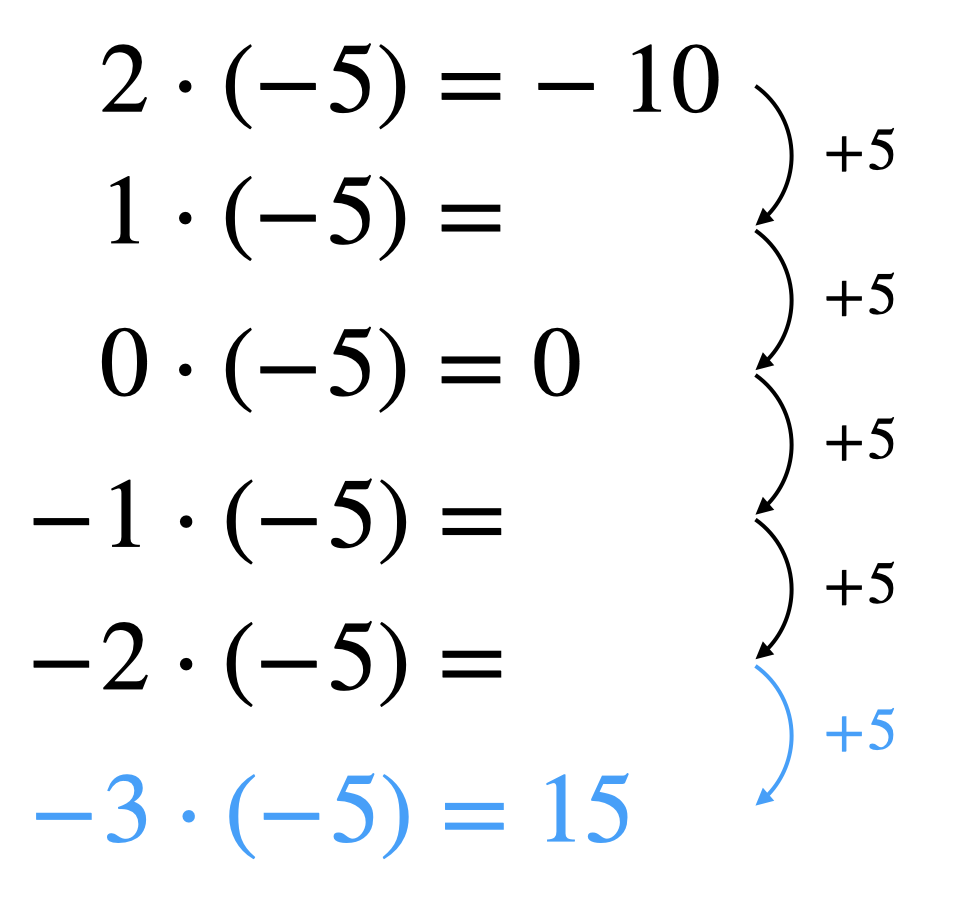
\includegraphics[width=0.3\linewidth]{pictures/2-Permanenz} 

}

\caption{Permanenzreihe zur Multiplikation zweier negativer Zahlen}\label{fig:Permanenz}
\end{figure}

Entscheidend ist beim Aufstellen von Permanenzreihen jedoch, dass der Übergang von einer Zeile zur nächsten auf einem entsprechenden Rechengesetz beruht. Im Abbildung \ref{fig:Permanenz} ist dies das Distributivgesetzt \((a-1) \cdot b = a \cdot b - b\). Varnachlässigt man die Existenz einer Übergangsregel, lassen sich plausibel erscheinende Muster fortsetzen (wie \(0^3 = 0\), \(0^2 = 0\), \(0^1 = 0\)), die dann allerdings zu falschen Schlussfolgerungen (\(0^0 = 0\)) führen. Im dargestellten Beispiel kann die Übergangsregel \(a^{m-1} = a^m : a\) wegen \(a = 0\) nicht angewandt werden.

\subsubsection{Ableitungen für den Lernpfad}\label{ableitungen-fuxfcr-den-lernpfad}

Aus all den bisherigen Überlegungen auf der formalen Ebene lassen sich für den Unterricht zentrale Fachinhalte ableiten:

\textcolor{formalColor}{Ganze Zahlen können über Zahlenpaare aus den natürlichen Zahlen oder als »Gegenzahlen« der natürlichen Zahlen entwickelt werden.}

\begin{itemize}
\tightlist
\item
  \textcolor{formalColor}{Natürliche Zahlen sind als Teilmenge in die ganzen Zahlen eingebettet.}
\item
  \textcolor{formalColor}{Die Subtraktion natürlicher Zahlen $m-n$ mit $n > m$ ist nun lösbar.}
\item
  \textcolor{formalColor}{Die Rechenregeln werden erweitert, wobei die bekannten weiter gelten. Die wird über das Permanenzprinzip begleitet, bei der Herleitung von Rechenregeln bietet sich die Nutzung von Permanenzreihen an.}
\end{itemize}

\subsection{Rationale Zahlen}\label{rationale-zahlen}

In fachlich analoger Weise lassen sich auch die rationalen Zahlen über Äquivalenzrelationen einführen. Dann fordert die »Quotientengleichheit«, dass für \(k,l,m,n\in\mathbb{N}\) mit \(l,n\neq 0\) gilt: \((k,l)\sim (m,n):\Leftrightarrow k\cdot n=l\cdot m\). Die Äquivalenzklasse \([(1,2)]\) kann dann mit \(\frac{1}{2}\) bezeichnet werden. Im Gegensatz zu den ganzen Zahlen ist es bei den rationalen Zahlen durchaus üblich, für dieselbe Zahl unterschiedliche Bezeichner zu verwenden, wie \(\frac{1}{2}\) oder \(\frac{5}{10}\). Fachmathematisch ist dies jedoch nicht relevant, also auch keine Diskussion auf der formalen Ebene (jedoch auf späteren Ebenen).

Aus Sicht der formalen Ebene lässt sich daher auch nicht ableiten, ob im Mathematikunterricht nach den natürlichen Zahlen zunächst die rationalen Zahlen (wie z.~B. in Deutschland) oder erst die ganzen Zahlen (wie z.~B. in Australien) eingeführt werden sollten. Innerhalb eines Zahlbereichs bietet jedoch die fachlogische Struktur Ansatzpunkte zur Gestaltung des Lernpfads, wie bei den negativen Zahlen dargestellt.

\section{Zum Nachbereiten}\label{mathematik-strukturieren-nachbereitung}

\begin{enumerate}
\def\labelenumi{\arabic{enumi}.}
\tightlist
\item
  Nutzen Sie verschiedene fachmathematische und fachdidaktische Quellen sowie Schulbücher, um fachlich zu klären, was »Terme« und »Gleichungen« sind.
\item
  Nutzen Sie Permanenzreihen, um weitere Rechengesetze nachzuvollziehen, z.~B. dass \(a^0 = 1\) (\(a\neq 0\)) und \(a^\frac{1}{2} = \sqrt{a}\) (\(a \geq 0\)) ist.
\item
  Wählen Sie eine Leitidee aus den Bildungsstandards aus und nennen Sie innerhalb dieser Begriffe, Zusammenhänge und Verfahren, die im Mathematikunterricht behandelt werden.
\end{enumerate}

\chapter{Grundvorstellungen}\label{grundvorstellungen}

\begin{quote}
\textbf{Ziele}

\begin{itemize}
\tightlist
\item
  Sie können die Grundvorstellungsidee beschreiben und wissen über deren Bedeutung für den Mathematikunterricht.
\item
  Ihnen ist bewusst, dass Grundvorstellungen i.~d.~R. zu Begriffen (Objekten und Operationen) existieren.
\item
  Sie kennen Grundvorstellungen zu einzelnen mathematischen Begriffen.
\end{itemize}

\textbf{Material}

\begin{itemize}
\tightlist
\item
  Folien zum Kapitel 3 (\href{files/Stoffdidaktik2024-03-Grundvorstellungen.pdf}{pdf}, \href{files/Stoffdidaktik2024-03-Grundvorstellungen.key}{Keynote})
\end{itemize}
\end{quote}

\section{Begriffsklärung}\label{grundvorstellungen-begriffsklaerung}

\subsection{Grundvorstellungsidee}\label{grundvorstellungsidee}

Als Sie zu Beginn Ihres Mathematikstudiums die Peano-Axiome zur Definition der natürlichen Zahlen \(\mathbb{N}\) kennengelernt haben, konnten Sie dies wahrscheinlich -- trotz der Neuigkeit der formalen Beschreibung -- derart mit Ihrer Lebenswelterfahrung in Verbindung bringen, dass natürliche Zahlen abgezählt werden können, also dass damit z.~B. die Platzierungen eines Wettrennens durchnummeriert werden können.

\begin{quote}
\textbf{Peano-Axiome} (\citeproc{ref-WikiPeano}{Wikipedia, 2021})

\begin{enumerate}
\def\labelenumi{\arabic{enumi}.}
\tightlist
\item
  \(0\) ist eine natürliche Zahl.
\item
  Jede natürliche Zahl \(n\) hat eine natürliche Zahl \(n'\) als Nachfolger.
\item
  \(0\) ist kein Nachfolger einer natürlichen Zahl.
\item
  Natürliche Zahlen mit gleichem Nachfolger sind gleich.
\item
  Enthält die Menge \(X\) die \(0\) und mit jeder natürlichen Zahl \(n\) auch deren Nachfolger \(n'\), so bilden die natürlichen Zahlen eine Teilmenge von \(X\).
\end{enumerate}
\end{quote}

Dieser \textbf{Bezug auf eine bekannte Handlung} ist wesentlich dafür, dass die Definition und damit der Begriff der natürlichen Zahlen für Sie mit einem Sinn behaftet ist. Innerhalb dieser \emph{ordinalen Sichtweise} natürlicher Zahlen helfen nun geeignete\footnote{\emph{Geeignet} heißt in diesem Fall, dass sich die Kernaussage des Begriffs in der Repräsentation wiederfindet. Im Ordinalzahlaspekt ist dies v.~a. die Reihung von Zahlen. Was dabei (noch) nicht relevant ist, ist zum Beispiel die exakte Messbarkeit, wie man sie etwa auf dem Zahlenstrahl repräsentiert.} \textbf{Repräsentationen} dabei, sich Rechenoperationen vorstellen und sie \textbf{operativ}\footnote{\emph{Operativ} heißt hier zum Beispiel, dass Sie zu einer Aufgabe wie \(2+7\) Nachbaraufgaben (\(2+8\)), Umkehraufgaben (\(7-2\)), Platzhalteraufgaben (\(2+\boxed{\phantom{5}}=7\)) usw. aufstellen und lösen können.} auszuführen zu können, also bspw. das Addieren als ein Weiterzählen aufzufassen (siehe Abbildung \ref{fig:Addition}).\index{Natürliche Zahlen|)}

\begin{figure}

{\centering 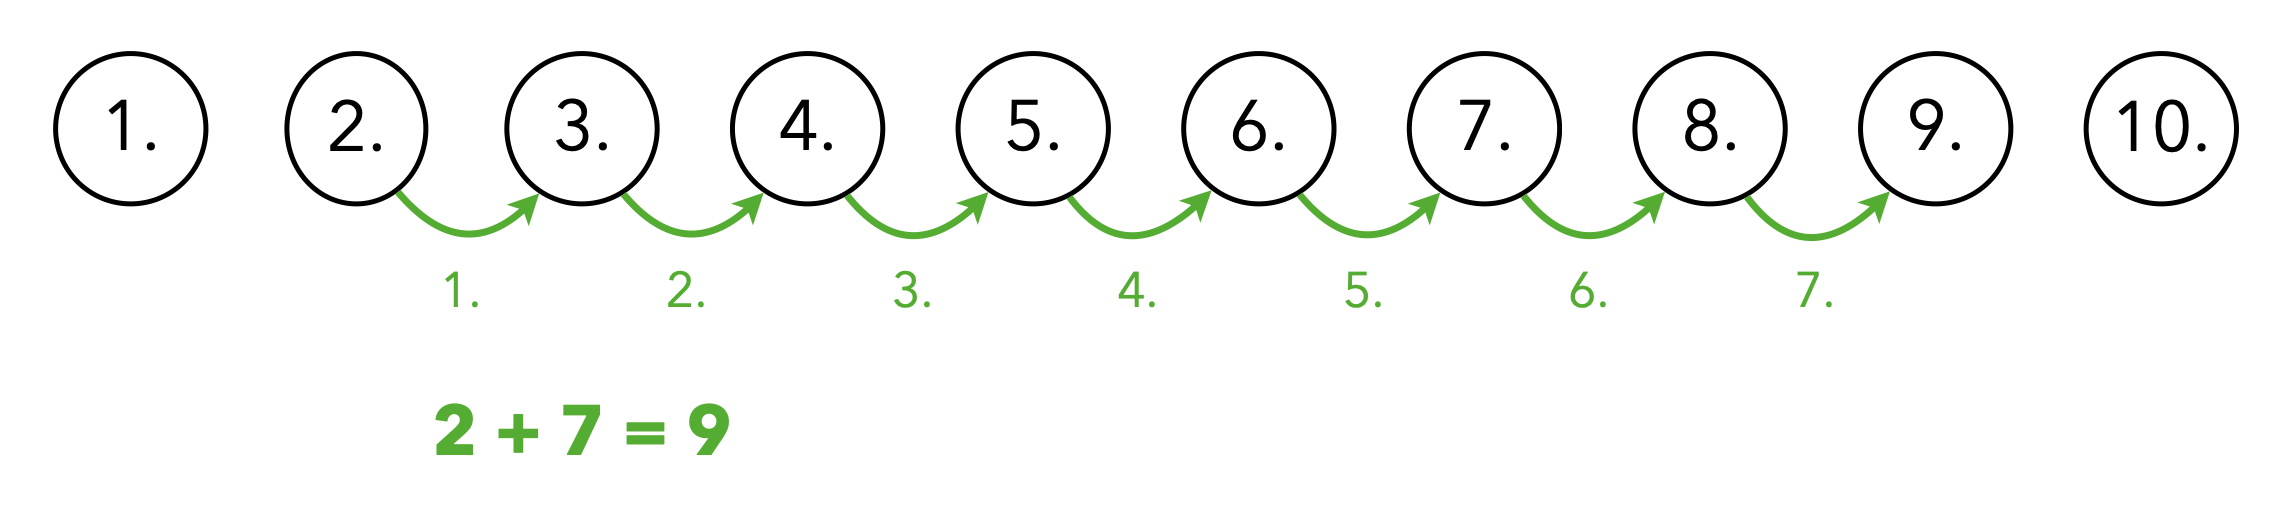
\includegraphics[width=0.75\linewidth]{pictures/4-Addition} 

}

\caption{Additionsaufgabe im ordinalen Zahlaspekt}\label{fig:Addition}
\end{figure}

Mit der Fähigkeit der Verknüpfung des mathematischen Begriffs und der Lebenswelt ist also eine \textbf{Anwendung des Begriffs auf die Wirklichkeit} möglich, insbesondere in Modellierungsprozessen. Dabei sind beide Richtungen relevant: Von der Realsituation zur Mathematik und von der Mathematik zur Realität.

Ziel des Mathematikunterrichts sollte es nun sein, für alle relevanten mathematischen Begriffe ein derartiges Verständnis aufzubauen, was auch heißt, verschiedene Vorstellungen zu einem Begriff zu vermitteln. Nach vom Hofe (\citeproc{ref-Hofe:1995}{1995, 97~f.}, Hervorhebung durch H.E.) ergibt sich daraus eine Orientierung an Grundvorstellungen im Mathematikunterricht:

\begin{definition}[Grundvorstellungen]
\protect\hypertarget{def:Grundvorstellungen}{}\label{def:Grundvorstellungen}

Die \textbf{Grundvorstellungsidee}\index{Grundvorstellung|textbf}\index{Grundvorstellungsidee|see{Grundvorstellung}} beschreibt \textbf{Beziehungen zwischen mathematischen Inhalten und} dem Phänomen der \textbf{individuellen Begriffsbildung}. In ihren unterschiedlichen Ausprägungen charakterisiert sie mit jeweils unterschiedlichen Schwerpunkten insbesondere drei Aspekte dieses Phänomens:

\begin{itemize}
\tightlist
\item
  Sinnkonstituierung eines Begriffs durch \textbf{Anknüpfung an} bekannte \textbf{Sach- oder Handlungszusammenhänge} bzw. \textbf{Handlungsvorstellungen},\index{Grundvorstellung!Sinnkonstituierung|textbf}
\item
  Aufbau entsprechender (visueller) \textbf{Repräsentationen bzw. »Verinnerlichungen«}, die \textbf{operatives Handeln} auf der Vorstellungsebene ermöglichen,\index{Grundvorstellung!Repräsentation|textbf}
\item
  Fähigkeit zur Anwendung eines Begriffs auf die Wirklichkeit durch \textbf{Erkennen der} entsprechenden \textbf{Struktur in Sachzusammenhängen} oder durch \textbf{Modellieren} des Sachproblems \textbf{mit Hilfe der mathematischen Struktur}.\index{Grundvorstellung!Modellierung|textbf}
\end{itemize}

\end{definition}

\subsection{Ausdifferenzierung}\label{ausdifferenzierung}

Weiterhin unterscheidet vom Hofe (\citeproc{ref-vomHofe2014}{2014}) zwischen \textbf{primären}\index{Grundvorstellung!primäre Grundvorstellung} und \textbf{sekundären}\index{Grundvorstellung!sekundäre Grundvorstellung} Grundvorstellungen, abhängig von der Erfahrungswelt der Handlungen. Während sich primäre Grundvorstellungen auf reale Handlungserfahrungen stützen (z.~B. mit Steckwürfeln in der Arithmetik), entstammen sekundäre Grundvorstellungen aus den Handlungen mit bereits im Mathematikunterricht aufgebauten Repräsentationen (z.~B. Operationen auf dem Zahlenstrahl).

Einige Quellen unterscheiden zwischen \textbf{Aspekten} und \textbf{Grundvorstellungen}. Nach Greefrath et al. (\citeproc{ref-Greefrath2016}{2016, S. 17}) ist ein »Aspekt eines mathematischen Begriffs {[}\ldots{]} ein Teilbereich des Begriffs, mit dem dieser fachlich
charakterisiert werden kann«, während »eine Grundvorstellung zu einem mathematischen Begriff {[}\ldots{]} eine inhaltliche Deutung des Begriffs {[}ist{]}, die diesem Sinn gibt.« Im oben angebrachte Beispiel entspräche die Definition der natürlichen Zahlen über die Peano-Axiome dem \emph{Ordinalzahlaspekt}, der mit der Grundvorstellung verbunden ist, dass die natürlichen Zahlen mit \(0\) beginnend eine feste Reihenfolge beschreiben. Da jedoch nicht alle Quellen diese Unterscheidung so präzise vornehmen und es auch teils zu Vermischungen kommt, soll diese (auf theoretischer Ebene relevante) Diskussion hier in der Stoffdidaktik-Veranstaltung nicht weiter von Relevanz sein. Für Ihre Unterrichtsgestaltung ist insbesondere relevant, dass sie einen \textbf{aspektreichen bzw. an vielfältigen Grundvorstellungen} orientierten Umgang mit Begriffen anstreben. Auch wenn Sie nicht unmittelbar und sofort jeweils alle Aspekte eines Begriffs im Unterricht ansprechen werden, hilft Ihnen das Wissen über den Aspektreichtum in der Unterrichtsplanung für die Ausbildung eines umfassenden Begriffsverständnisses.

Entsprechend ihrer Definition werden Grundvorstellungen für \textbf{Begriffe} erarbeitet -- hinsichtlich der Arten mathematischen Wissens (vgl. Abschnitt \ref{arten-mathematischen-wissens}) also anscheinend nicht für Zusammenhänge und Verfahren. Jedoch können Grundvorstellungen zu einem Begriff sowohl hinsichtlich des \emph{Objekts} an sich bestehen, als auch hinsichtlich der \emph{Operationen} mit diesem Begriff. Das Addieren ist beispielsweise im Ordinalzahlaspekt eine Operation, verbunden mit der Grundvorstellung des Weiterzählens. Insofern können auch Zusammenhänge und Verfahren durchaus mit Grundvorstellungen verknüpft werden, sofern der Fokus auf dem Operieren mit den in ihnen enthaltenen Begriffen liegt.

Die in Definition \ref{def:Grundvorstellungen} dargestellte Grundvorstellungsidee hat einen \textbf{normativen}\index{Grundvorstellung!normativ|textbf} Charakter, d.~h. es wird davon ausgegangen, dass (aus professioneller Sicht der Mathematikdidaktik) zu mathematischen Begriffen bestimmte Grundvorstellungen identifiziert werden können, die es im Unterricht zu vermitteln gilt. Oder anders gefragt: »Welche Grundvorstellungen sind zur Lösung des Problems aus der Sicht des Lehrenden adäquat?« (\citeproc{ref-Hofe:1995}{vom Hofe, 1995, S. 106}). Diese Sichtweise wird durch eine \textbf{deskriptive}\index{Grundvorstellung!deskriptiv|textbf} Perspektive ergänzt: »Welche individuellen Vorstellungen lassen sich im Lösungsversuch des Schülers erkennen?« (\citeproc{ref-Hofe:1995}{vom Hofe, 1995, S. 107}). Diese über empirische Untersuchungen zu ermittelnden Vorstellungen sind das, was sich Schülerinnen und Schüler \emph{tatsächlich} unter einem Begriff vorstellen, wozu ggf. auch typische \emph{Fehlvorstellungen}\footnote{Mit \emph{Fehlvorstellungen} sind hier individuelle Vorstellungen der Schülerinnen und Schüler gemeint, die mathematisch nicht tragfähig und daher aus fachlicher Perspektive fehlerhaft sind. So ist etwa die Vorstellung, dass Multiplizieren immer vergrößert, in den Natürlichen Zahlen tragfähig (und damit eine Grundvorstellung), in den Bruchzahlen jedoch nicht mehr tragfähig und wird dort dann zur Fehlvorstellung. Neben \emph{Fehlvorstellungen} können weitere individuelle Vorstellungen \emph{Alltagsvorstellungen}, \emph{Präkonzepte} o.~ä. sein (siehe auch \citeproc{ref-Schecker2018}{Schecker et al., 2018, 11~f.}).} gehören können. Kenntnisse darüber sind für Lehrkräfte ungemein wichtig, um Ergebnisse von Schülerinnen und Schülern interpretieren und einordnen zu können und dann ggf. entsprechende Hilfsangebote zu machen. Dies entspricht dann einer \textbf{konstruktiven}\index{Grundvorstellung!konstruktiv|textbf} Perspektive auf Grundvorstellungen: »Worauf sind etwaige Divergenzen zurückzuführen, und wie lassen sich diese beheben?« (\citeproc{ref-Hofe:1995}{vom Hofe, 1995, S. 107}).

\section{GV und Stoffdidaktik}\label{gv-und-stoffdidaktik}

Im Rahmen dieser Veranstaltung, insbesondere den von Ihnen ausgearbeiteten Seminarthemen, wird der Schwerpunkt auf \emph{normative} Grundvorstellungen gelegt, was der \textcolor{semanticColor}{semantischen Ebene} des \hyperref[tab:fragen-ebenen]{Vier-Ebenen-Ansatzes} zugeordnet werden kann, weil die mathematischen Begriffe hier mit einem Sinn versehen werden. Die \emph{deskriptive} und \emph{konstruktive} Perspektive sind dagegen der \textcolor{empiricColor}{empirischen Ebene} zuzuordnen, da hier individuelle Vorstellungen der Schülerinnen und Schüler von Relevanz sind. Dies betrifft insbesondere auch das Potenzial, (ggf. mathematisch unvollständige) individuelle Vorstellungen aufzugreifen bei der Ausbildung von (normativ erwünschten) Grundvorstellungen.

Das Identifizieren von Grundvorstellungen zu einem Begriff ist, genau wie bei den \hyperref[fundamentale-ideen]{Fundamentalen Ideen}, Aufgabe der mathematikdidaktischen Forschung (ein Modell dafür findet man bei \citeproc{ref-Salle2021}{Salle \& Clüver, 2021}). Als Lehrkraft profitieren Sie von diesen Ergebnissen und nutzen sie für Ihre stoffdidaktische Analyse.

Im Gegensatz zu den fundamentalen Ideen, die ihren Ursprung in der \emph{Sachstruktur des mathematischen Inhalts} haben, fokussieren die Grundvorstellungen stärker auf den Sinn des fachlichen Begriffs \emph{für das Individuum}. Grundvorstellungen beziehen sich auf spezifische Begriffe und Operationen mit Begriffen, während fundamentale Ideen größere, themenübergreifende Leitlinien für die Stoffauswahl und -strukturierung bilden.

Für die Unterrichtsplanung und -durchführung ist neben der Frage, \emph{welche} Grundvorstellungen von Relevanz sind (Spezifizieren im Vier-Ebenen-Ansatz) vor allem interessant, \emph{wie} diese ausgebildet werden können (Strukturieren im Vier-Ebenen-Ansatz). Letzteres wird u.~a. in den nächsten Kapiteln näher beleuchtet.

\section{Beispiele}\label{beispiele}

\subsection{Natürliche Zahlen}\label{natuxfcrliche-zahlen-1}

Betrachten Sie folgenden (fiktiven) Zeitungsartikel:\index{Natürliche Zahlen|(}

\begin{quote}
\textbf{\emph{Harlequin erneut auf dem 1. Platz}}

\emph{Bei dem traditionellen Pferderennen am 15. Mai hat das Pferd Harlequin erneut gewonnen. Unter den 10 Pferden, die an den Start gingen, belegte es mit 21,3 Sekunden den 1. Platz. Damit war es fast 2 mal so schnell unterwegs wie das letzte Pferd, das ins Ziel kam. Karten für das nächste Rennen können unter 030 23125143 bestellt werden.}
\end{quote}

In dem Text tauchen Zahlen unter vielen Aspekten auf: Der \textbf{1.} Platz und \textbf{15.} Mai sind \textbf{Ordinalzahlen}, also Zahlen, die eine Ordnung beschreiben. Wie oben schon beschrieben, lassen diese sich fachmathematisch über die Peano-Axiome beschreiben und wenn mit ihnen gerechnet, entspricht z.~B. das Addieren dem \textbf{Weiterzählen}.

Die \textbf{10} Pferde stellen eine \textbf{Kardinalzahl} dar, also die Anzahl der Elemente einer Menge. Addiert man Kardinalzahlen, so müssen \textbf{Mengen vereinigt} werden, z.~B. anschaulich, indem man sie zusammen legt.

Die \textbf{21,3} Sekunden entsprechen einer \textbf{Maßzahl}, da diese Zahl die Funktion hat, etwas auszumessen (hier die Zeit). Das Addieren in diesem Aspekt entspräche dem \textbf{Aneinanderlegen}, z.~B. wenn zwei Längenangaben addiert werden.

Dass es \textbf{2} mal so schnell wird, enspricht einem \textbf{Operatoraspekt}, mit dem die Vielfachheit eines Vorganges beschrieben wird. Das Addieren ist hierin eine \textbf{Hinereinanderausführung} eines Vorganges.

Die Telefonnumer \textbf{030 23125143} wiederum erfüllt einen \textbf{Codierungsaspekt}. Sie hat im mathematischen Sinne keine Bedeutung, nur die Anordnung der Ziffern ist von Relevanz. Entsprechend kann innerhalb dieses Aspektes auch nicht addiert werden. Weitere Beispiele hierfür wären Postleitzahlen oder Identifikationsnummern.

Hinzu kommt noch der Aspekt der \textbf{Rechenzahl}. Informationen dazu sowie eine genauere Erläuterung der Zahlaspekte und damit verbundenen Operationen findet man z.~B. bei Krauthausen (\citeproc{ref-Krauthausen:2018}{2018, 43~ff.}).\index{Natürliche Zahlen|)}

\subsection{Bruchzahlen}\label{bruchzahlen}

Nachdem\index{Brüche|(} die Schülerinnen und Schüler ihr gesamte Vorschul- und Primarstufenzeit mit Natürlichen Zahlen verbracht haben, treten mit der Einführung von Bruchzahlen Umbrüche in den subjektiven Vorstellungen auf. Zum Beispiel sind folgende (vermeintlichen) Gesetzmäßigkeiten plötzlich \emph{nicht mehr} gültig:

\begin{itemize}
\tightlist
\item
  Das Produkt zweier Zahlen ist größer als die jeweiligen Faktoren.
\item
  Die Multiplikation kann als wiederholte Addition aufgefasst werden.
\item
  Jede Zahl hat genau einen Repräsentanten.
\item
  Je mehr Stellen eine Zahl hat, desto größer ist sie.
\end{itemize}

Die Bruchzahlen selbst besitzen nach Padberg \& Wartha (\citeproc{ref-Padberg:2017}{2017, 19~ff.}) folgende Aspekte:

\begin{itemize}
\tightlist
\item
  Bruch als \textbf{Anteil eines Ganzen} oder \textbf{mehrerer Ganzer}
  (z.~B. \(\frac{2}{3}\) als zwei Drittel einer Pizza oder je ein Drittel von zwei Pizzen),
\item
  Bruch als \textbf{Maßzahl}
  (z.~B. \(\frac{1}{4}\) Liter),
\item
  Bruch als \textbf{Operator}
  (z.~B. \(\frac{1}{5}\) von 250 €),
\item
  Bruch als \textbf{Verhältnis}
  (z.~B. \(\frac{2}{3}\) mit der Bedeutung \emph{2 von 3 Schüler/-innen tragen eine Brille}),
\item
  Bruch als \textbf{Quotient}
  (z.~B. \(\frac{3}{5}\) als Ergebnis bzw. andere Schreibweise von \(3:5\)),
\item
  Bruch als \textbf{Lösung einer linearen Gleichung}
  (z.~B. \(\frac{3}{5}\) als Lösung von \(5x = 3\)),
\item
  Bruch als \textbf{Skalenwert}
  (z.~B. \(\frac{3}{2}\) als Mitte zwischen \(1\) und \(2\) auf dem Zahlenstrahl),
\item
  \textbf{Quasikardinale Auffassung} von Brüchen
  (z.~B. \(\frac{3}{5}\) als 3 mal \(\frac{1}{5}\)).
\end{itemize}

Neben den Grundrechenoperationen führt auch das Vergleichen von Brüchen zu Grundvorstellungsumbrüchen. Hinzu kommen noch besondere Operationen mit Bruchzahlen wie das Erweitern und Kürzen.

Das Multiplizieren von Brüchen kann bspw. als Anteilsbildung (\(\frac{1}{5}\) mal \ldots{} heißt \(\frac{1}{5}\) \emph{von} \ldots) oder als Rechteckfläche aufgefasst werden (\citeproc{ref-Padberg:2017}{Padberg \& Wartha, 2017, 108~ff}), siehe Abbildung \ref{fig:Bruchmultiplikation}.

\begin{figure}

{\centering 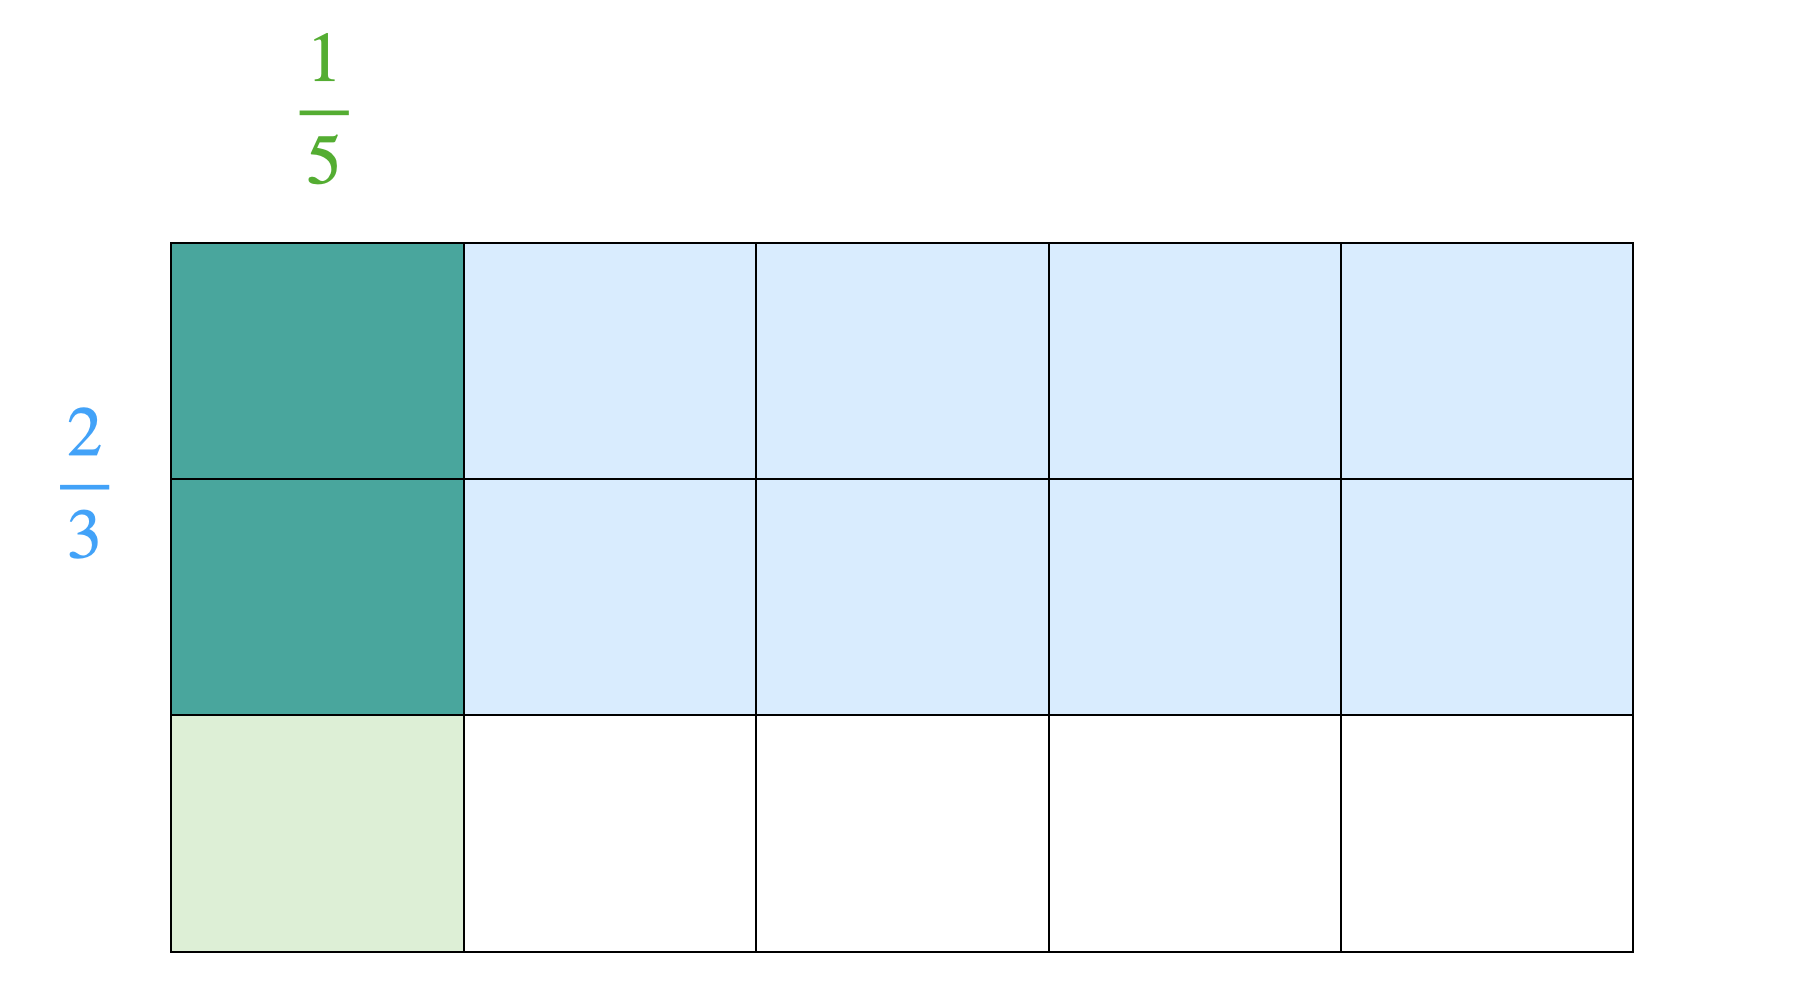
\includegraphics[width=0.5\linewidth]{pictures/4-Bruchmulti} 

}

\caption{Vorstellung von $\frac{1}{5} \cdot \frac{2}{3}$ als Rechteckfläche}\label{fig:Bruchmultiplikation}
\end{figure}

All dies zeigt, dass Brüche behutsam unterrichtet werden sollten und von einer rein kalkülorientierten Behandlung unbedingt abgesehen werden muss, da diese den nachhaltigen Lernerfolg deutlich mindert.\index{Brüche|)}

\subsection{Negative Zahlen}\label{negative-zahlen}

Aufbauend auf die in Abschnitt \ref{beispiel-negative-zahlen} erfolgte Diskussion zur \textcolor{formalColor}{formalen Ebene} von negativen Zahlen, soll zu diesen nun die Grundvorstellungsidee auf der \textcolor{semanticColor}{semantischen Ebene} diskutiert werden.

Die Einführung negativer Zahlen ist für Schülerinnen und Schüler mit zahlreichen Schwierigkeiten verbunden (\citeproc{ref-vomHofe2014a}{vom Hofe \& Hattermann, 2014}). Diese sind eigentlich auf der \textcolor{empiricColor}{empirischen Ebene} der stoffdidaktischen Analyse angesiedelt, sollen aber hier wegen ihrer Nähe zu den Grundvorstellungen schon einmal erwähnt werden.

\begin{itemize}
\tightlist
\item
  So bestehen etwa für das \textbf{Minus-Zeichen vielfältige Interpretationsmöglichkeiten} als \textbf{Vorzeichen} (z.~B. in der Rechnung \(-5+2\)), als \textbf{Rechenzeichen} (z.~B. in der Rechnung \(7-2\)) oder als \textbf{Inversionszeichen} (z.~B. bei der Darstellung \(-a\) als Gegenzahl für \(a\)).
\item
  Der in den natürlichen Zahlen vorhandene \textbf{Kardinalzahlaspekt} (dass die Zahl die Mächtigkeit einer Menge angibt), ist in den negativen Zahlen \textbf{nicht mehr tragfähig} (es existiert keine \(-4\)-elementige Menge). Auch der \textbf{Ordinalzahlaspekt} (dass die Zahl eine Position angibt) ist nur \textbf{eingeschränkt tragfähig} (eine \(-4\)-te Position bedarf vielfältiger Zwischeninterpretationen). Der \textbf{Maßzahlaspekt} (z.~B. über die Angabe einer Zahl auf dem Zahlenstrahl) dagegen ist auf die negativen Zahlen \textbf{erweiterbar}.
\item
  Die \textbf{Ordnungsrelation} wird häufig \textbf{fehlinterpretiert} über eine spiegelbildliche Interpretation (z.~B. kann fälschlicherweise \(-5>-3\) angenommen werden). Eine Ursache kann hier darin liegen, dass die Ordnungsrelation zuvor über die Mächtigkeit von Mengen hergestellt wurde, was nun nicht mehr möglich ist.
\end{itemize}

Gegenüber den natürlichen Zahlen sind also im Umgang mit negativen Zahlen einige Grundvorstellungsumbrüche zu absolvieren. Als normativ auszubildende Grundvorstellungen fassen vom Hofe \& Hattermann (\citeproc{ref-vomHofe2014a}{2014}) für rationale Zahlen (als Obermenge positiver und negativer Zahlen) zusammen:

\begin{itemize}
\tightlist
\item
  Rationale Zahlen als \textbf{relative Zahlen bezüglich einer fest gewählten Vergleichsmarke}: Dies ist etwa bei Etagen-Angaben, Temperaturen oder der Position über/unter dem Wasserspiegel der Fall. Gerade bei Temperaturen kann die Beliebigkeit der Vergleichsmarke (0~°C) gut diskutiert werden, da etwa andere Temperaturskalen (°F, K) eine andere Vergleichsmarke gewählt haben.
\item
  Rationale Zahlen als \textbf{Gegensätze}: Diese Vorstellung wird z.~B. sichtbar, wenn über Guthaben und Schulden gesprochen wird. Hat man 5~€ Schulden, so ist dies der Gegensatz von 5~€ Guthaben. Die Vergleichsmarke (0~€) ist hier nicht beliebig gewählt, sondern natürlicherweise über »weder Guthaben noch Schulden« gegeben. Auch der Betrag einer Zahl kann in dieser Vorstellung besonders gut verstanden werden.
\item
  Rationale Zahlen als \textbf{Richtungen}: Negative Zahlen beschreiben in dieser Vorstellung die entgegengesetzte Richtung der positiven Zahlen. Dies ist z.~B. bei der Verwendung von Koordinatensystemen der Fall, oder ganz allgemein bei der Zahlengeraden.
\item
  Rationale Zahlen als \textbf{Zustände und Zustandsänderungen}: In dieser Vorstellung bieten rationale Zahlen nicht nur die Möglichkeit, einen Zustand (wie Guthaben oder Schulden) zu beschreiben, sondern auch den Prozess der Änderung dieser Zustände (Erhalt von Guthaben, Erlass von Schulden, \ldots). Eine solche Vorstellung etwa ist nötig, um die verschiedenen Interpretationen des Minus-Zeichens nachvollziehen zu können.
\end{itemize}

Als bedeutsamste Repräsentation negativer Zahlen gilt die Zahlengerade. Diese stützt einerseits den Maßzahlaspekt und ermöglicht über die Darstellung von Punkten und Pfeilen (siehe Abbildung \ref{fig:Zahlengerade}) auch eine Interpretation in den verschiedenen Grundvorstellungen.

\begin{figure}

{\centering 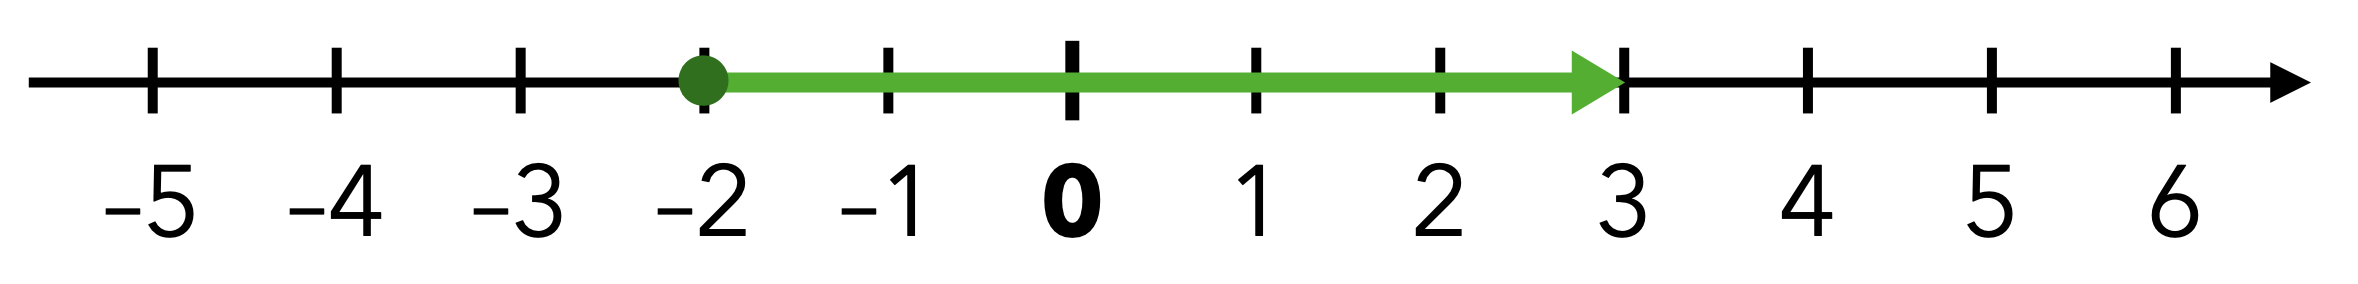
\includegraphics[width=0.75\linewidth]{pictures/4-Zahlengerade} 

}

\caption{Zahlengerade}\label{fig:Zahlengerade}
\end{figure}

Auch Operationen mit negativen Zahlen sind hierzu nun verständlich behandelbar:

\begin{itemize}
\tightlist
\item
  So kann das \textbf{Addieren/Subtrahieren} als Anlegen von Pfeilen, gerichtetes Weiter-/Zurückzählen oder als Subtraktion/Addition der Gegenzahl aufgefasst werden.
\item
  Das \textbf{Multiplizieren} kann bei der Multiplikation mit einer positiven Zahl als Streckung/Stauchung aufgefasst werden, die Multiplikation mit \(-1\) entspricht der Spiegelung an der Null und die Multiplikation mit einer beliebigen negativen Zahl ist eine Kombination aus beidem.
\item
  Der \textbf{Größenvergleich} ist nun über einen Lagevergleich auf der Zahlengeraden möglich, wobei weiter links liegende Zahlen immer kleiner sind als weiter rechts liegende.
\end{itemize}

Zusammenfassend lassen sich auf der semantischen Ebene folgende für den Lernpfad relevanten Zusammenhänge ableiten:

\begin{itemize}
\tightlist
\item
  \textcolor{semanticColor}{Rationale Zahlen sollten als relative Zahlen bezüglich einer fest gewählten Vergleichsmarke, als Gegensätze, als Richtungen sowie als Zustände und Zustandsänderungen aufgefasst werden können.}
\item
  \textcolor{semanticColor}{Die Zahlengerade ist eine wesentliche Repräsentation rationaler Zahlen, anhand derer auch die Operationen mit rationalen Zahlen sichtbar gemacht werden können.}
\end{itemize}

\section{Zum Nachbereiten}\label{grundvorstellungen-nachbereitung}

Bearbeiten Sie folgende Aufgaben entweder am Begriff \emph{Variable} oder am Begriff \emph{Term}. Als Quelle sei Weigand et al. (\citeproc{ref-Weigand2022}{2022}) zu empfehlen.

\begin{enumerate}
\def\labelenumi{\arabic{enumi}.}
\tightlist
\item
  Informieren Sie sich über die Grundvorstellungen zum gewählten Begriff.
\item
  Arbeiten Sie heraus, inwiefern die Aspekte der Grundvorstellungsidee erfüllt werden, d.~h.

  \begin{itemize}
  \tightlist
  \item
    stellen Sie die Sinnhaftigkeit des Begriffs durch mögliche Handlungserfahrungen dar,
  \item
    finden Sie geeignete Repräsentationen, anhand derer operatives Handeln ermöglicht wird und
  \item
    beschreiben Sie mögliche Modellierungsprozesse des Begriffs mithilfe der gewählten Grundvorstellung.
  \end{itemize}
\item
  Diskutieren Sie, ob es sich um primäre oder sekundäre Grundvorstellungen handelt.
\end{enumerate}

\chapter{Kernideen und Kontexte}\label{kernideen-und-kontexte}

\begin{quote}
\textbf{Ziele}

\begin{itemize}
\tightlist
\item
  Sie kennen das Konzept von Kernideen als das Wesen des Lerngegenstands.
\item
  Sie kennen Kernideen zu einzelnen Lerngegenständen.
\item
  Sie können gegebene Kontexte zu Lerngegenständen hinsichtlich ihrer Sinnstiftung beurteilen.
\item
  Sie sind sich der Möglichkeiten und Bedeutung horizontaler und vertikaler Mathematisierung bewusst.
\end{itemize}

\textbf{Material}

\begin{itemize}
\tightlist
\item
  Folien zum Kapitel 4 (\href{files/Stoffdidaktik2024-04-KernideenUndKontexte.pdf}{pdf}, \href{files/Stoffdidaktik2024-04-KernideenUndKontexte.key}{Keynote})
\end{itemize}
\end{quote}

\section{Begriffsklärung Kernidee/-frage}\label{kernidee-begriffsklaerung}

\textbf{Kernideen} haben die Aufgabe, den Lernpfad zu leiten und dabei das \emph{Wesen} des neuen Lerngegenstands sichtbar zu machen. Sie müssen dabei sowohl aus objektiver (also mathematischer) Perspektive tragfähig sein, als auch aus subjektiver Perspektive für die Schülerinnen und Schüler greifbar werden können. Kernideen bieten damit im \emph{Vorfeld} des Lernpfades eine Orientierung und im \emph{Nachgang} des Lernpfades eine Reflexionsmöglichkeit über den Lerngegenstand.\footnote{Der Begriff der Kernidee ist geprägt worden über das Dialogische Lernen nach Gallin und Ruf, spricht dort jedoch vorwiegend die Vorschauperspektive an (vgl. \citeproc{ref-Leuders2011}{Leuders et al., 2011, S. 7}).} Um bei den Schülerinnen und Schülern Lernprozesse zu einem Lerngegenstand zu initiieren, werden die Kernideen ansprechend in Form von \textbf{Kernfragen} formuliert. Kernfragen sollten daher prinzipiell aus subjektiver Sicht formuliert sein und insbesondere adressieren, wie man selbst mit dem Lerngegenstand umgehen kann.

Am Beispiel des \emph{Funktionsbegriffs}\index{Funktionsbegriff} etwa besteht eine Kernidee darin, dass Funktionen den Zusammenhang zwischen zwei Größen beschreiben und damit auch vorhersagen können (vgl. auch Aspekte des Funktionsbegriffs in einem späteren Kapitel). Als Kernfrage formuliert: »Wie kann man die Beziehung zwischen zwei sich verändernden Größen beschreiben und wie kann man damit weitere Werte bestimmen?« (\citeproc{ref-Thiel-Schneider2018}{Thiel-Schneider, 2018, S. 49}).

In der \emph{Vorschauperspektive} heißt das, die »Kernidee in Frageform schließt an individuelle Vorerfahrungen, Zielperspektiven, Denk- und Handlungsmuster der Lernenden an und initiiert die Auseinandersetzung mit dem mathematischen Gegenstand in den Worten von Schülerinnen und Schülern« (\citeproc{ref-Leuders2011}{Leuders et al., 2011, S. 8}). In der \emph{Rückschauperspektive} dagegen können über die Kernidee (dann quasi als Antwort auf die Kernfrage) »eine allgemeine Problemstellung und die zu ihrer Bewältigung notwendigen mathematischen Konzepte benannt« werden (\citeproc{ref-Leuders2011}{Leuders et al., 2011, S. 8}).

\begin{definition}[Kernidee und Kernfrage]
\protect\hypertarget{def:Kernidee}{}\label{def:Kernidee}Eine \textbf{Kernidee}\index{Kernidee|textbf} beschreibt in wenigen Worten das Wesen eines Lerngegenstands, d.~h. sie beschreibt, was den Lerngegenstand aus formaler und semantischer Perspektive auszeichnet -- insbesondere in Abgrenzung zu thematisch ähnlichen Lerngegenständen.

Eine \textbf{Kernfrage}\index{Kernfrage|textbf} stellt die Kernidee in Frageform aus der Perspektive der Schülerinnen und Schüler dar.

Kernideen und Kernfragen verfolgen eine \textbf{\emph{Vorschauperspektive}}\index{Kernidee!Vorschauperspektive|textbf}, die der Orientierung und Initiierung der Auseinandersetzung mit dem neuen Lerngegenstand dient, sowie eine \textbf{\emph{Rückschauperspektive}}\index{Kernidee!Rückschauperspektive|textbf}, die es den Schülerinnen und Schülern ermöglicht, den Lerngegenstand einzuordnen.
\end{definition}

Bestandteil Ihrer stoffdidaktischen Analyse auf der \textcolor{concreteColor}{konkreten Ebene} wird es also sein, zum Lerngegenstand passende Kernideen zu identifizieren und in Form von Kernfragen zu formulieren. Hierzu kann Ihnen die Sinnkonstituierung der jeweiligen Grundvorstellungen dienlich sein (siehe Definition \ref{def:Grundvorstellungen}).

\section{Begriffsklärung Kontext}\label{kontexte-begriffsklaerung}

\textbf{Kontexte} sollen geeignet sein, sich dem Lerngegenstand exemplarisch zu nähern. Sie weisen damit immer eine Spezialisierung bzw. Konkretisierung des zu betrachtenden Lerngegenstands auf (denn nur so können die Schülerinnen und Schüler einen Zugang dazu finden) -- sollen aber so gestaltet sein, dass an Ihnen das Allgemeine erfahrbar ist (denn nur so kann es zu einer Beschäftigung mit der dahinterliegenden Mathematik kommen). Es wird dann auch von einem \emph{sinnstiftenden Kontext} gesprochen.

Leuders et al. (\citeproc{ref-Leuders2011}{2011, S. 4}, Hervorhebungen im Original) formulieren hierzu:

\begin{definition}[Sinnstiftender Kontext]
\protect\hypertarget{def:Kontext}{}\label{def:Kontext}

Ein \textbf{sinnstiftender Kontext}\index{Kontext|textbf} ist ein Ausschnitt einer inner- oder außermathematischen Welt, der folgende Anforderungen möglichst gut erfüllt:

\begin{itemize}
\tightlist
\item
  Er ist anschlussfähig an die Erfahrungen, Interessen und die Denk- und Handlungsmuster der Lernenden \textbf{(Lebensweltbezug)}.\index{Kontext!Lebensweltbezug|textbf}
\item
  Er ermöglicht es, authentische Fragen zu bearbeiten und dabei auch etwas über den Kontext zu lernen \textbf{(Kontextauthentizität)}.\index{Kontext!Kontextauthentizität|textbf}
\item
  Er ist problemhaltig und offen genug, um Lernende zum reichhaltigen Fragen und Erkunden anzuregen \textbf{(Reichhaltigkeit)}.\index{Kontext!Reichhaltigkeit|textbf}
\end{itemize}

\end{definition}

Um einer eingeschränkten Sichtweise vorzubeugen, sei gesagt: Der \emph{Lebensweltbezug} heißt nicht zwingend, dass es sich um einen \emph{Realitätsbezug} (im Sinne einer Modellierung) handeln muss. Dies ist zwar in vielen Fällen angebracht, aber auch eine innermathematische Anschlussfähigkeit kann für die Schülerinnen und Schüler ansprechend sein (und damit Bezug zu deren -- schulischen -- Leben herstellen).

Ein möglicher Kontext, über den die oben formulierte Kernfrage bei \emph{linearen Funktionen}\index{Lineare Funktion}\index{Funktionsbegriff!Lineare Funktion|see{Lineare Funktion}} erarbeitet werden kann, wäre die Beschreibung des Abbrennverhaltens einer Kerze (vgl. \citeproc{ref-Boeer2014}{Böer et al., 2014, 108~f}). Dieser ist für die Schülerinnen und Schüler aus dem Alltag bekannt (wenn auch nicht alltäglich). Authentisch und reichhaltig ist der Kontext dahingehend, dass die meisten Kerzen zylinderförmig sind und daher tatsächlich ein lineares Abbrennverhalten haben. Auch ist es durchaus von Interesse, die Zeit bis zum vollständigen Abbrennen einer Kerze abschätzen zu können (z.~B. bei einer \emph{Kerzenuhr}, vgl. \citeproc{ref-WikiKerze}{Wikipedia, 2022a}). Weiterhin können (später) die Eigenschaften des Funktionsgraphen kontextgebunden interpretiert werden (\(y\)-Achsenabschnitt als Ursprungslänge der Kerze, Nullstelle als die Zeit bis zum vollständigen Abbrennen, Anstieg des Graphen als Abbrennverhalten, das direkt mit der Dicke der Kerze in Verbindung gebracht werden kann).

Das Finden derartiger stinnstiftender Kontexte ist enorm anspruchsvoll! Sie sollten hier auf (gute) Lehrwerke zurückgreifen und immer wieder mögliche Kontexte kritisch (mithilfe der Definition \ref{def:Kontext}) hinterfragen.

Kernideen/Kernfragen und der sinnstiftende Kontext bilden damit eine Einheit in der \textbf{Motivierung und Zielbildung} zu Beginn der Auseinandersetzung mit einem Lerngegenstand, siehe auch einen späteren Abschnitt hier im Skript.

\section{Mathematisierungstypen}\label{mathematisierungstypen}

Während Kernideen, Kernfragen und Kontexte in erster Linie der \emph{Spezifizierung} des Lerngegenstandes in Hinblick auf den Lernpfad dienen, kann zur \emph{Strukturierung} der Prozess der Mathematisierung stärker in den Blick genommen werden. Angelehnt an Treffers und Freudenthal stellt van den Heuvel-Panhuizen (\citeproc{ref-vandenHeuvel-Panhuizen2003}{2003, S. 12}) hierzu dar, dass prinzipiell zwei Wege der Mathematisierung möglich sind:

\begin{itemize}
\item
  Bei der \textbf{horizontalen Mathematisierung}\index{Horizontale Mathematisierung} werden mithilfe mathematischer Objekte und Operationen reale Situationen und alltägliche Probleme beschrieben, geordnet und gelöst. Es wird also aus der Welt des Lebens in die Welt der Symbole übergegangen.\footnote{im Original: »In the case of horizontal mathematizing, mathematical tools are brought forward and used to organize and solve a problem situated in daily life. {[}\ldots{]} to mathematize horizontally means to go from the world of life to the world of symbols« (\citeproc{ref-vandenHeuvel-Panhuizen2003}{van den Heuvel-Panhuizen, 2003, S. 12})}
\item
  Bei der \textbf{vertikalen Mathematisierung}\index{Vertikale Mathematisierung} wird innerhalb des mathematischen Systems reorganisiert und operiert, es wird sich also in der Welt der Symbole bewegt.\footnote{im Original: »Vertical mathematizing, on the contrary, stands for all kinds of re-organizations and operations done by the students within the mathematical system itself. {[}\ldots{]} to mathematize vertically means to move within the world of symbols« (\citeproc{ref-vandenHeuvel-Panhuizen2003}{van den Heuvel-Panhuizen, 2003, S. 12})}
\end{itemize}

Beide Arten sind nicht als Konkurrenten aufzufassen, sondern haben ihre gleiche Berechtigung im Mathematikunterricht. Dies ist v.~a. vor dem Hintergrund zu verstehen, dass Mathematik \emph{vom Menschen betrieben} wird. Erst durch das Zusammenwirken von horizontaler und vertikaler Mathematisierung kann Mathematik unter dieser Annahme auf ehrliche Weise durchgeführt und damit auch verstanden werden. Dies heißt insbesondere, dass in jeder Klassenstufe beide Arten der Mathematisierung ihre Berechtigung haben und entsprechend realisiert werden müssen.\footnote{im Original: »Freudenthal emphasized, however, that the differences between these two worlds are far from clear cut, and that, in his view, the worlds are not, in fact, separate. Moreover, he found the two forms of mathematizing to be of equal value, and stressed the fact that both activities could take place on all levels of mathematical activity.« (\citeproc{ref-vandenHeuvel-Panhuizen2003}{van den Heuvel-Panhuizen, 2003, S. 12})}

Das oben dargestellte Kerzenbeispiel entstammt der horizontalen Mathematisierung. Eine vertikale Mathematisierung könnte bspw. im weiteren Lernverlauf -- etwa nachdem die Funktionsgleichung \(y = m\cdot x + n\) eingeführt wurde -- die Untersuchung des Einflusses der Parameter \(m\) und \(n\) auf den Funktionsgraphen sein. Daran zeigt sich schon, wie hilfreich eine gleichermaßen Betrachtung horizontaler und vertikaler Prozesse ist, nämlich wenn etwa nach einer Veränderung von \(m\) und \(n\) rückgefragt wird, inwieweit dies noch mit den Abbrennen einer Kerze in Zusammenhang steht (was spätestens bei einem positiven \(m\) an seine Grenzen stößt). Derartige \emph{Grenzbetrachtungen} (die mathematisch greifbar sind, aber in der Realität eben an ihre Grenzen stoßen) bieten ein enormes Potenzial, sich dem abstrakten Wesen von Mathematik zu nähern.

\section{Zum Nachbereiten}\label{kernideen-kontexte-nachbereitung}

\begin{enumerate}
\def\labelenumi{\arabic{enumi}.}
\tightlist
\item
  Entwickeln Sie für den Begriff der \emph{Exponentialfunktion} eine Kernfrage.
\item
  Untersuchen Sie, inwieweit folgende Kontexte für Exponentialfunktionen sinnstiftend sind:

  \begin{itemize}
  \tightlist
  \item
    Bakterienwachstum
  \item
    Bierschaumzerfall
  \end{itemize}
\item
  Beschreiben und erklären Sie je eine geeignete Variante der horizontalen und vertikalen Mathematisierung am Lerngegenstand der Exponentialfunktion.
\end{enumerate}

\part*{Lernprozesse gestalten}\label{part-lernprozesse-gestalten}
\addcontentsline{toc}{part}{Lernprozesse gestalten}

\chapter{Lernprozesse auslösen}\label{lernprozesse-ausluxf6sen}

\begin{quote}
\textbf{Ziele}

\begin{itemize}
\tightlist
\item
  Sie kennen Möglichkeiten zur Motivierung und Zielbildung, um Lernprozesse bei Schülerinnen und Schülern auszulösen.
\item
  Sie können die verschiedenen Qualitäten der Orientierungsbildung beschreiben und erkennen Orientierungshilfen als Unterstützungsinstrumente höherwertiger Orientierungsbildung.
  +Sie können unterrichtspraktische Herangehensweisen zum Auslösen von Lernprozessen lernpsychologisch begründen.
\end{itemize}

\textbf{Material}

\begin{itemize}
\tightlist
\item
  Folien zum Kapitel 5 (\href{files/Stoffdidaktik2024-05-LernprozesseAusloesen.pdf}{pdf}, \href{files/Stoffdidaktik2024-05-LernprozesseAusloesen.key}{Keynote})
\end{itemize}
\end{quote}

\section{Lerntätigkeit und Lernhandlung}\label{lerntaetigkeit-und-lernhandlung}

Eine Grundannahme der Tätigkeitstheorie, die auf Vygotskijs psychologische Arbeiten aus den 1920er Jahren in der Sowjetunion zurück geht, ist das Verständnis, dass sich \textbf{Individuen aktiv-handelnd mit ihrer Umwelt auseinandersetzen}, \textbf{die Umwelt} dabei in der Interaktion mit der Gesellschaft \textbf{verändern}, und beide Prozesse wiederum psychisch im Individuum abgebildet werden. Dies widerspricht bspw. der \emph{behavioristischen} Annahme, dass man sich seiner Umwelt einfach nur anpasst, aber es ist auch nicht mit einer \emph{streng konstruktivistischen} Annahme zu verwechseln, nach der Individuen ein Abbild der Umwelt kognitiv rekonstruieren. Die Tätigkeitstheorie kann eher als »(moderat) konstruktivistische{[}r{]}{[}..{]} Ansatz« bezeichnet werden (\citeproc{ref-Giest2016a}{Giest, 2016, S. 47}).

Zu betonen ist dabei die \textbf{beiderseitige Wirkrichtung}: Sowohl das Individuum wirkt auf die Umwelt ein (und verändert sie, es kommt zur \emph{gesellschaftlichen Weiterentwicklung}), als auch die Umwelt auf das Individuum (was zur \emph{Persönlichkeitsentwicklung} führt). Beide Prozesse sind dabei nicht voneinander zu trennen. Eine solche Interaktion ist von (gesellschaftlich entwickelten) Motiven geprägt und wird als \textbf{\emph{Tätigkeit}} bezeichnet. Giest \& Lompscher (\citeproc{ref-Giest2006}{2006, S. 27}) formulieren: »Er {[}der Mensch{]} erschafft damit seine Kultur und zugleich die psychischen Funktionen, die ihn dazu in die Lage versetzen.« Dieses Paradoxon, dass die Tätigkeit ihre eigene Voraussetzung ist, kann aufgelöst werden, indem man zunächst kultur-historisch die gemeinschaftliche und erst dann die individuelle Tätigkeit betrachtet: »Durch (gemeinsame) Tätigkeit erfolgte die (kulturelle) Menschwerdung und über ihre individuelle Aneignung verläuft die Persönlichkeitsentwicklung« (\citeproc{ref-Giest2006}{Giest \& Lompscher, 2006, S. 27}).

Für schulische Prozesse von besonderem Interesse ist die \textbf{\emph{Lerntätigkeit}}, in der Definition nach Giest \& Lompscher (\citeproc{ref-Giest2006}{2006, S. 67}):

\begin{definition}[Lerntätigkeit]
\protect\hypertarget{def:Lerntaetigkeit}{}\label{def:Lerntaetigkeit}Lerntätigkeit kann man definieren als die speziell auf die Aneignung gesellschaftlichen Wissens und Könnens (Lerngegenstände) gerichtete Tätigkeit, wozu spezifische Mittel (Lernmittel) unter speziell gestalteten Bedingungen eingesetzt werden müssen.
\end{definition}

Giest \& Lompscher (\citeproc{ref-Giest2006}{2006, S. 67}) führen fort: »Da die Lerngegenstände und Lernmittel kultureller Natur sind, kann Lerntätigkeit auch nur im Rahmen der Kultur, der Kooperation und Kommunikation mit denen, die über diese Kultur verfügen, angeeignet werden.« Dies betont in der Unterrichtsrealität u.~a. die besondere Bedeutung und Verantwortung der Lehrkraft als wissende Person, die den Lernprozess der Schülerinnen und Schüler steuert. Dies heißt nicht, dass Unterricht lehrerzentriert gestaltet werden soll, ganz im Gegenteil: Entscheidend ist, dass die Lehrperson die Schülerinnen und Schüler dazu befähigt, sich den Lerngegenstand anzueignen, etwa indem sie geeignete Lernmittel zur Verfügung stellt und den Umgang mit ihnen schult.

Auch unabhänging vom Lernen sind Tätigkeiten stets auf einen \textbf{Gegenstand} bezogen, können also niemals inhaltsleer erfolgen. Tätigkeiten basieren dabei auf \textbf{Motiven}, d.~h. »innere Antriebe« (\citeproc{ref-Giest2006}{Giest \& Lompscher, 2006, S. 39}). Im Kontext des Lernens sind dies insbesondere die Motive \emph{Interesse}, \emph{Leistung}, \emph{Affiliation} (soziale Nähe) und \emph{Neugierde} (\citeproc{ref-Mienert2011}{Mienert \& Pitcher, 2011, S. 57}). In der Konfrontation mit einem Gegenstand bildet das Individuum, basierend auf die Motive, \textbf{Ziele} als »ideell vorweggenommene Resultate der Tätigkeit« aus (\citeproc{ref-Giest2006}{Giest \& Lompscher, 2006, S. 39}), was zu \textbf{Handlungen} im Zusammenhang mit dem Gegenstand führt. Handlungen dienen also der (zielgerichteten) Realisierung der Tätigkeit.
Im Rahmen der \emph{Lerntätigkeit} führt dies dann zu \textbf{\emph{Lernhandlungen}}. Lompscher (\citeproc{ref-Lompscher1985b}{1985, S. 46}) definiert:

\begin{definition}[Lernhandlung]
\protect\hypertarget{def:Lernhandlung}{}\label{def:Lernhandlung}Lernhandlungen sind relativ geschlossene und abgrenzbare, zeitlich und logisch strukturierte Abschnitte im Verlauf der Lerntätigkeit, die ein konkretes Lernziel realisieren, durch bestimmte Lernmotive angetrieben werden und entsprechend den konkreten Lernbedingungen durch den Einsatz äußerer und verinnerlichter Lernmittel in einer jeweils spezifischen Folge von Teilhandlungen vollzogen werden.
\end{definition}

Aufbauend auf Lernziele können nun Lernhandlungen ausgebildet (also ausgeführt und verinnerlicht) werden. So können etwa als \emph{Elementare Aneignungshandlungen} das \textbf{Identifizieren} und \textbf{Realisieren} genannt werden. Idenzifizieren ist die Prüfung der Passung eines gegebenen Objekt zur einer vorgegebenen Objektklasse und Realisieren das Erzeugen eines entsprechenden Repräsentanten. Identifizierungs- und Realisierungshandlungen sind v.~a. bei der Erstbegegnung mit einem neuen Lerngegenstand -- insbesondere bei Begriffen -- von hoher Relevanz. Sie sind, in verinnerlichter Form, Voraussetzung für die noch folgenden Handlungsarten (und damit letztlich auch Bestandteile von ihnen).
Darauf aufbauend können \emph{Grundhandlungen} (\textbf{Erkennen}, \textbf{Beschreiben}, \textbf{Verknüpfen}, \textbf{Anwenden}\footnote{Um hier einer ggf. eingeschränkten Auffassung des Vorgehens bei Sach- oder Modellierungsaufgaben (»Anwenden auf die Realität«) vorzubeugen, sei auf die Beschreibung verwiesen: »Feststellen der Übereinstimmung von den Bedingungen der Aufgabenstellung mit der Ausgangskonstellation der zu realisierenden gegebenen (oder erzeugten) Handlungsvorschrift (Identifizieren) und ggf. Herstellen einer solchen Übereinstimmung (Transferieren)« (\citeproc{ref-Feldt-Caesar2017}{Feldt-Caesar, 2017, S. 93})} und \textbf{Begründen}) sowie \emph{komplexe Handlungen} (\textbf{Suchen}, \textbf{Planen}, \textbf{Ausführen} und \textbf{Kontrollieren}) erfolgen. Diese Handlungen sind i.~d.~R. in Festigungs- und Vertiefungsphasen bzw. bei Modellierungs- und Problemlösesituationen von Relevanz. Diese Art der Handlungskategorisierung geht auf Bruder \& Brückner (\citeproc{ref-Bruder1989}{1989}) zurück und wird nahezu unverändert auch bei Feldt-Caesar (\citeproc{ref-Feldt-Caesar2017}{2017, 87~ff.}) dargestellt.



\begin{quote}
Am Beispiel des Winkelfeldes in Abschnitt \ref{konkrete-ebene} lautete eine Aufgabe für die Schülerinnen und Schüler: »Wo muss das Schaf lang laufen, damit es die gesamte Zeit gerade so von der Kuh gesehen wird?« Hierfür bewegen die Schülerinnen und Schüler in der App das Schaf entlang der Sichtfeldgrenze der Kuh, geradlinig und in Richtung der Augen der Kuh begrenzt und in die andere Richtung unbegrenzt. Sie \emph{identifizieren und realisieren} damit das mathematische Objekt \emph{Strahl}, gebunden am Kontext der Sichtfelder. Im Anschluss wird diese Handlung (kontextunabhängig) verallgemeinert und die Strahl-Eigenschaft des Schenkels charakterisiert.
\end{quote}

\begin{figure}

{\centering 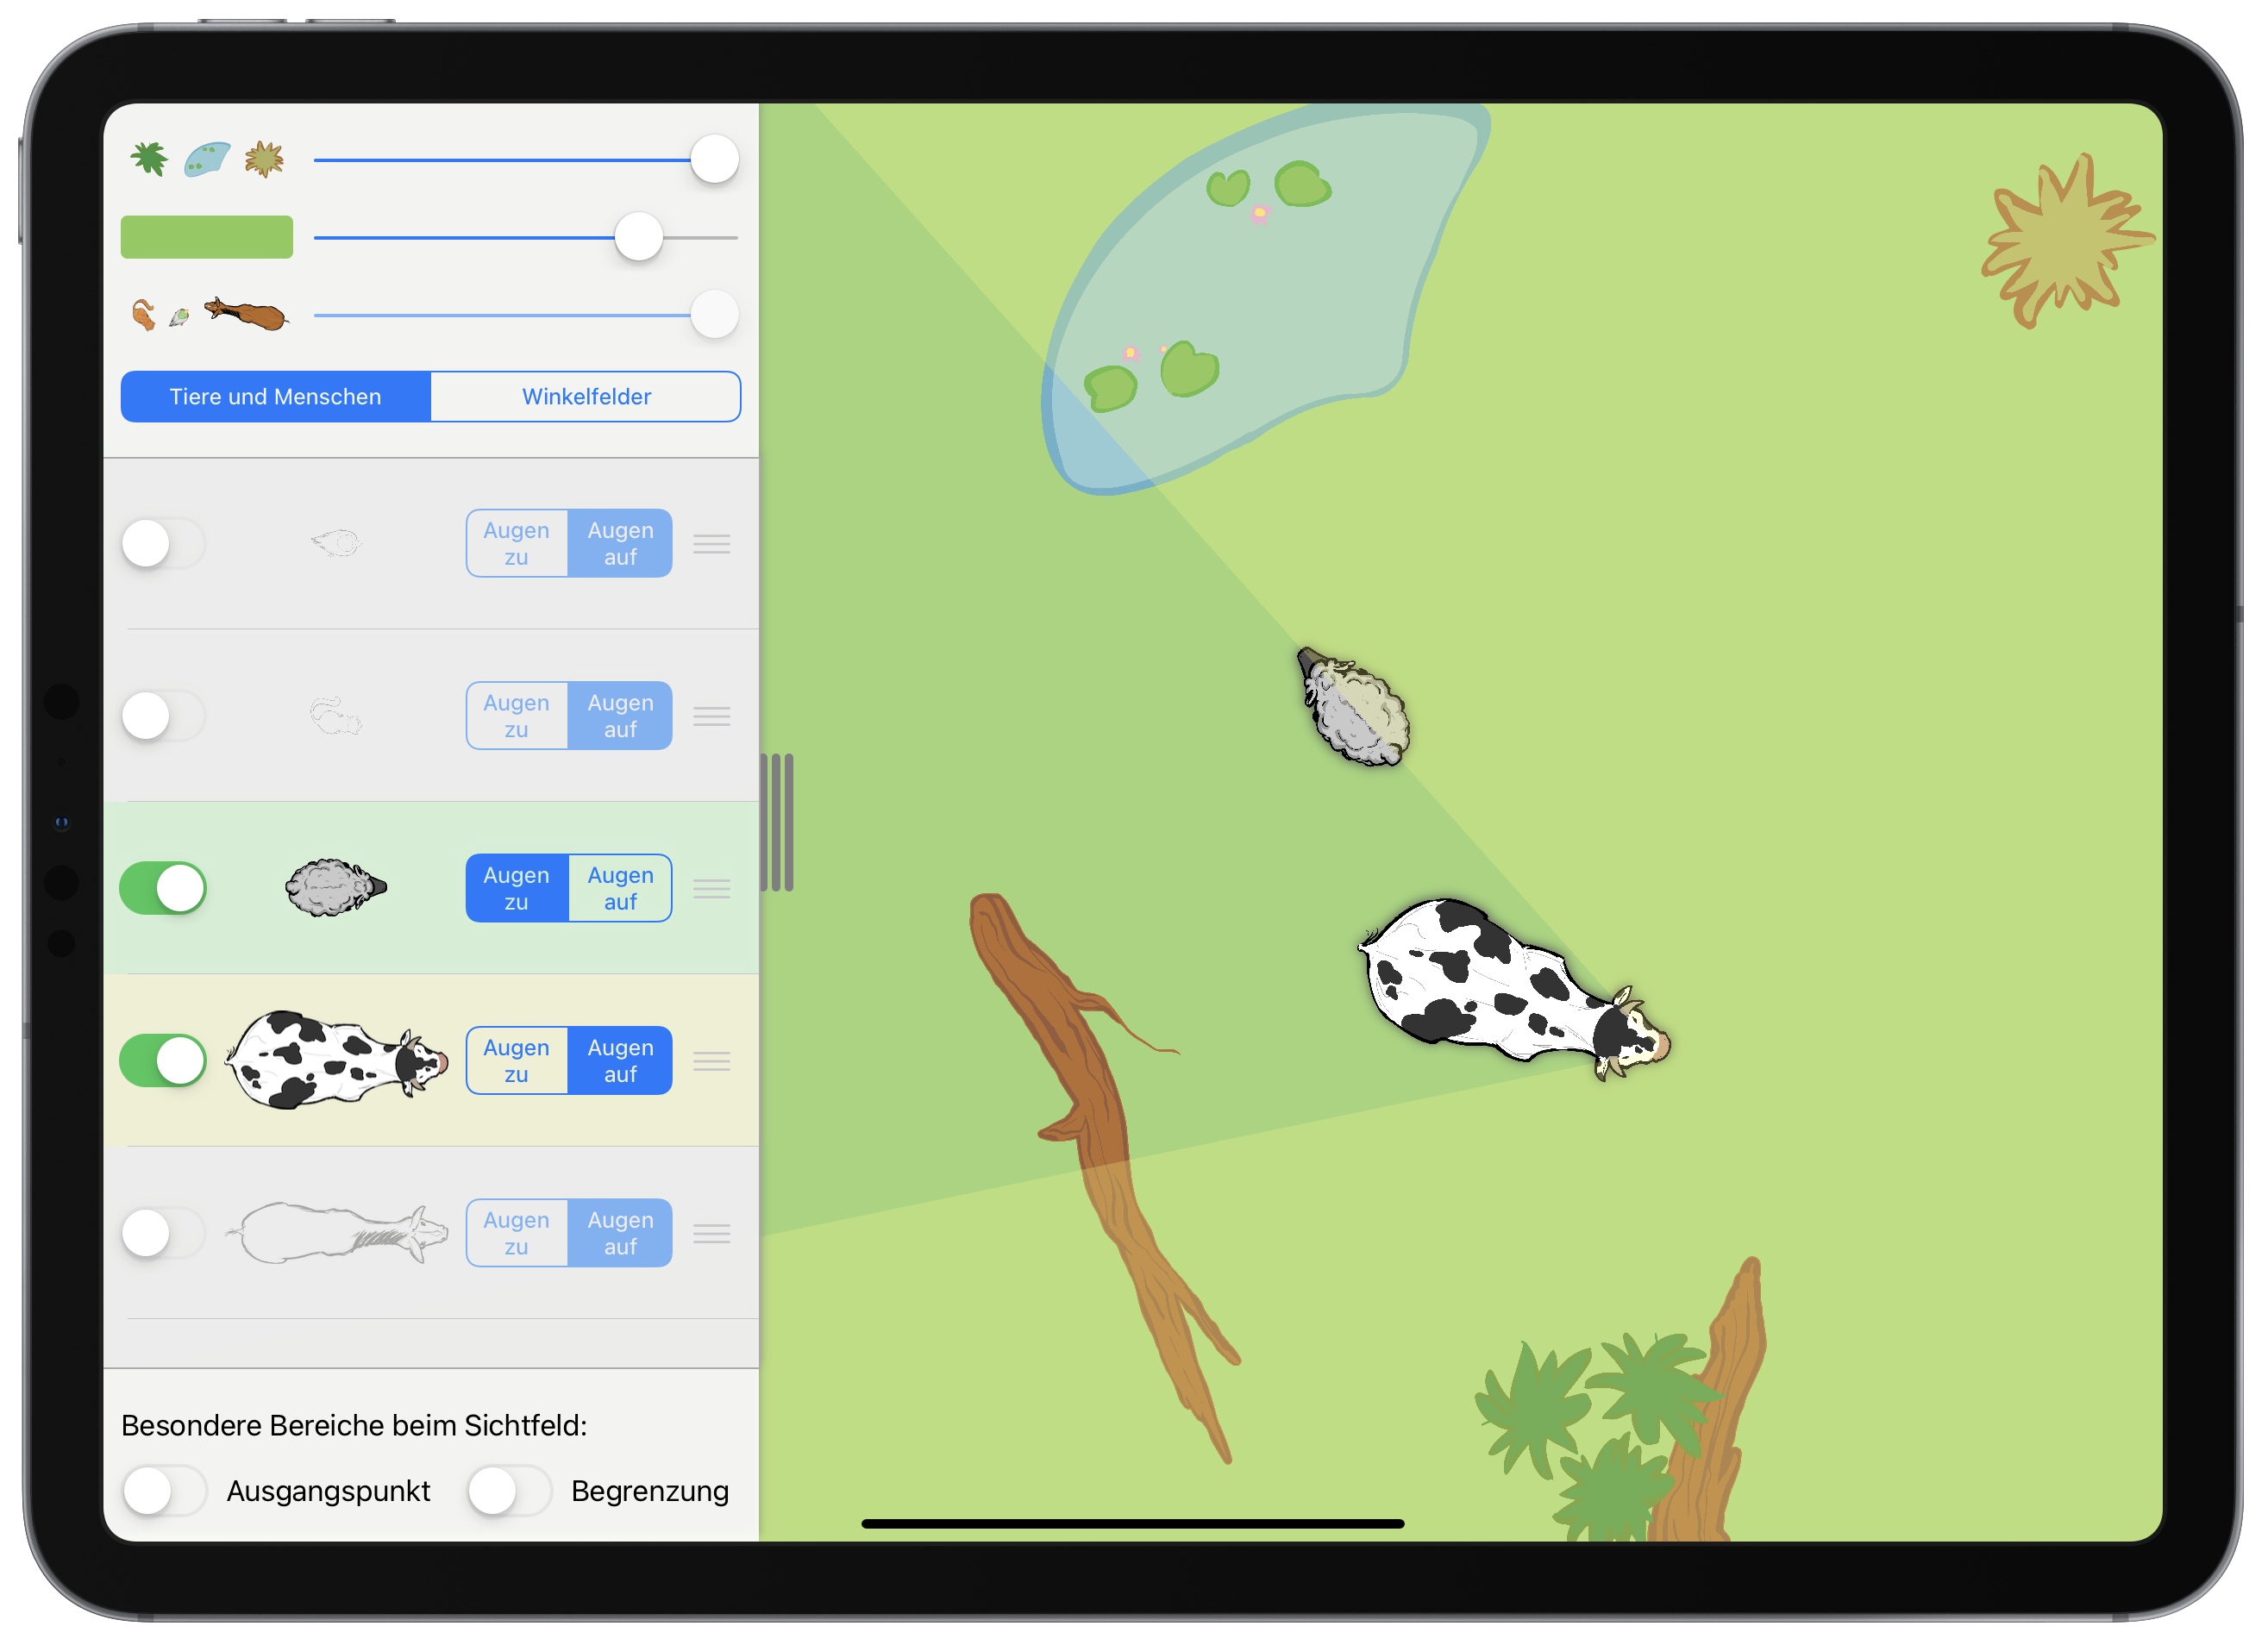
\includegraphics[width=0.5\linewidth]{pictures/1-Winkelfarm} 

}

\caption{Lernhandlung in der App \emph{Winkel-Farm} (\citeproc{ref-Etzold:2019}{Etzold, 2019a})}\label{fig:HandlungSchaf}
\end{figure}

Welche Schritte für die Ausbildung von Lernhandlungen notwendig sind, wird im nächsten Kapitel dargestellt.
Zu betonen ist, dass die Lernhandlungen zwar einerseits notwendig sind, um sich einem Lerngegenstand zu nähern, also die \textbf{Handlungen als \emph{Lernmittel}} aufgefasst werden können. Andererseits müssen die Lernhandlungen jedoch auch erst einmal ausgeprägt werden, also auch die \textbf{Handlungen als \emph{Lerngegenstand}} selbst aufgefasst werden (was wiederum nur am konkreten mathematischen Unterrichtsthema realisiert werden kann). Diese Sichtweise sollte Sie als Lehrkraft dafür sensibilisieren, dass Sie nicht per se davon ausgehen können, dass Ihre Schülerinnen und Schüler über entsprechende Handlungen verfügen, um neue mathematische Themen zu erlernen, sondern an diesen Themen die Handlungen erarbeitet und mit den Handlungen die Mathematik erarbeitet wird. Auch hier kann wieder von der zunächst gemeinschaftlichen Handlungsausführung (in der Klassensituation und mit Unterstützung von Personen, die über das anzueignende Wissen verfügen) zur individuellen Handlungsausführung (und damit persönlichen Aneignung des Lerngegenstands) übergegangen werden.

\section{Motivierung und Zielbildung}\label{motivierung-und-zielbildung}

Die obigen Überlegungen zeigen, dass die \textbf{Motivierung und Zielbildung} bedeutsame Bestandteile eines Lernprozesses sind, sich also in der Gestaltung konkreter Unterrichtssituationen widerspiegeln müssen -- durch entsprechende Phasen innerhalb einer Unterrichtsstunde. Erst wenn Motive und Ziele ausgeprägt sind, kann es in weiteren Unterrichtsphasen zur \textbf{Ausbildung der Lernhandlungen} kommen.

\subsection{Zone der nächsten Entwicklung}\label{zone-der-nuxe4chsten-entwicklung}

Die Schülerinnen und Schüler müssen zunächst in die Lage versetzt werden, sich mit dem Lerngegenstand auseinandersetzen zu \emph{wollen}. Hierzu ist es (aus lernpsychologischer Sicht) hilfreich, die Anforderungssituation in der \textbf{Zone der nächsten Entwicklung} der Schülerinnen und Schüler zu präsentieren. Dabei handelt es sich um eine Problemsituation, Aufgabe oder Fragestellung, die die Schülerinnen und Schüler zwar mithilfe ihrer bisherigen Kenntnisse, Fähigkeiten und Fertigkeiten \textbf{verstehen und nachvollziehen} können, zu ihrer Lösung sie jedoch noch \textbf{nicht selbstständig} (aber mit Unterstützung wissender Personen) in der Lage sind. Somit wird eine Motivation geschaffen, sich mit der Thematik tiefer auseinanderzusetzen. Es ist durchaus möglich, an dieser Stelle auch schon erste Lösungsversuche zu unternehmen. Daran ist besonders gut zu erkennen, »was wir nicht wissen bzw. können, um die Anforderung zu bewältigen« (\citeproc{ref-Lompscher1996}{Lompscher, 1996, S. 4}).

Dem kann die \textbf{Zone der aktuellen Leistung} gegenübergestellt werden, also Probleme bzw. Aufgaben, die die Schülerinnen und Schüler bereits selbstständig lösen können. Würde jedoch jede Anforderungssituation in der Zone der aktuellen Leistung liegen, wäre langfristig kein Lernzuwachs möglich (und insbesondere könnte sich keine Motivation zum Lernen einstellen).

Ein bestimmtes Niveau eines Individuums ist dadurch gekennzeichnet, dass es zu bestimmten Dingen selbstständig in der Lage ist, zu anderen jedoch noch nicht. Der Übergang zum nächst höheren Niveau erfolgt, indem die soeben noch nicht selbstständig lösbaren Problemstellungen (in der Zone der nächsten Entwicklung) zu selbstständig lösbaren Problemstellungen (in der Zone der aktuellen Leistung) werden. Ein solcher Niveauübergang erfolgt Lompscher (\citeproc{ref-Lompscher1985b}{1985, S. 26}) zufolge durch »pädagogische Führung«. Diese etwas sperrige Bezeichnung drückt jedoch nichts anderes aus, als dass die Lehrkraft für die Gestaltung des Lernprozesses verantwortlich ist, damit die Schülerinnen und Schüler den entsprechenden Niveauübergang vollführen können.



\begin{figure}

{\centering 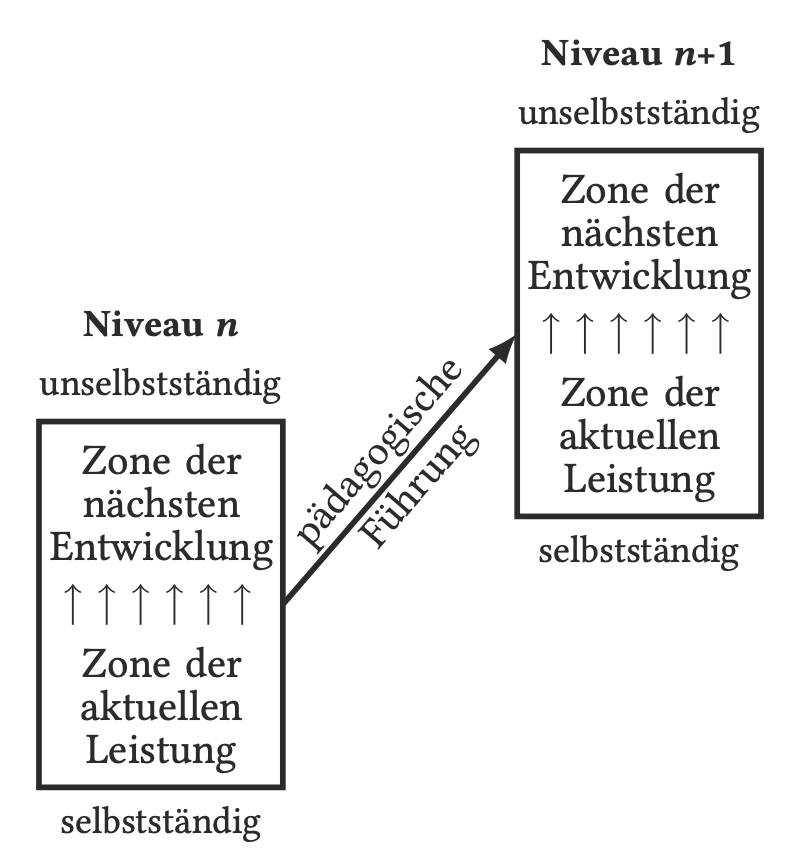
\includegraphics[width=0.5\linewidth]{pictures/5-ZdnE} 

}

\caption{Zone der nächsten Entwicklung (nach \citeproc{ref-Lompscher1985b}{Lompscher, 1985, S. 26})}\label{fig:ZdnE}
\end{figure}

\begin{quote}
Beim Winkelfeld wurden den Schülerinnen und Schülern Fotos verschiedener Tiere präsentiert, die teils ihre Augen an der Seite des Kopfes und teils nach vorn gerichtet hatten. Es wurde besprochen, was diese Tiere unterscheidet (Flucht- und Jagdtiere) und welche Bedeutung die Lage der Augen hierfür haben kann. Diese Situation ist für die Schülerinnen und Schüler nachvollziehbar, aber sie können noch nicht selbstständig beschreiben, welcher geometrische Zusammenhang zwischen der Position der Augen und der Lebensweise der Tiere besteht.
\end{quote}

\subsection{Lernzielbildung}\label{lernzielbildung}

Aus dem Motiv heraus, sich mit einem konkreten Lerngegenstand zu beschäftigen, erfolgt eine geistige Vorwegnahne, was das \emph{Ergebnis} der Lerntätigkeit ist. Darunter sind neue »Handlungen, Verhaltensweisen, Bedeutungen, Werte, Normen, Begriffe, Gesetzmäßigkeiten usw. in Form von Kenntnissen, Fähigkeiten, Einstellungen und anderen psychischen Eigenschaften« zu verstehen (\citeproc{ref-Lompscher1985b}{Lompscher, 1985, S. 40}). Solche (psychischen) Ergebnisse unterscheiden sich damit von (äußeren) \emph{Produkten} wie »Zeichnungen, schriftliche Arbeiten, Materialsammlungen, Werkstücke, mündliche Aussagen u.~a.« (\citeproc{ref-Lompscher1985b}{Lompscher, 1985, S. 40}).

Die Orientierung darauf, eines der \emph{Ergebnisse} zu erzielen, entspricht demnach dem \textbf{Lernziel}. Hier ist zu beachten, dass das \emph{Lernziel} nicht zu verwechseln ist mit dem von der Lehrkraft erwünschten \emph{Lehrziel}.\footnote{Erst recht nicht zu verwechseln ist der Begriff mit den »Lernzielen« außerhalb der Tätigkeitstheorie, die bspw. bei einer Unterrichtsplanung angegeben werden. Letztere entsprechen eher den Lehrzielen und können auch -- um Verwechslungen zu vermeiden -- als \emph{Kompetenzziele} bezeichnet werden, da sie Kompetenzen beschreiben, die am Ende der entsprechenden Unterrichtsstunde ausgebildet worden sein sollen.} Lernziele werden individuell von den Schülerinnen und Schülern ausgeprägt. Sie haben jedoch als Lehrkraft die Aufgabe, eine solche Lernzielbildung zu unterstützen und idealerweise auch zu lenken, so dass die Schülerinnen und Schüler für den Lerngegenstand adäquate Lernziele bilden. Der Grad der \textbf{Bewusstheit, Allgemeinheit und Differenziertheit} des Lernziels bestimmt dabei letztlich auch, in welcher Qualität die darauf basierenden Lernhandlungen ausgeprägt werden (vgl. \citeproc{ref-Lompscher1985b}{Lompscher, 1985, S. 43}). Möchte ein Kind einfach nur die Lösung der Aufgabe \(17+8\) ermitteln (Produktorientierung), so wird es nicht so qualitativ hochwertig und nachhaltig lernen können, als wenn es das Ziel verfolgt, grundsätzlich Additionsaufgaben mit Zehnerübergang lösen zu können (Ergebnisorientierung).

Es bietet sich eine \textbf{explizite Verbalisierung und auch das Festhalten von Lernzielen} (z.~B. an der Tafel) an, um während des Lernprozesses darauf zurückgreifen und seinen eigenen Handlungsfortschritt permanent mit den Zielen abgleichen zu können.

\begin{quote}
Anknüpfend an die Präsentation der Tierbilder zu Winkelfeldern wurde, von der Lehrkraft durch ein Lehrer-Schüler-Gespräch initiiert, als Lernziel formuliert: »Wir wollen Sichfelder von Tieren beschreiben und miteinander vergleichen« (vgl. \citeproc{ref-Etzold:2019Praxis4}{Etzold, 2019b, S. 6}). Diese Zielformulierung enthält bewusst keine mathematischen Fachbegriffe des neuen Lerngegenstandes, da diese zum entsprechenden Zeitpunkt ja noch gar nicht erarbeitet worden sind.
\end{quote}

Wie das Beispiel schon zeigt, müssen Motivierung und Zielbildung nicht als getrennte Unterrichtsphasen strukturiert werden. Relevant ist jedoch, \emph{dass} sie stattfinden und einen bedeutsamen Raum im Unterricht einnehmen. Ein Unterrichtsbeginn mit »Wir beschäftigen uns heute mit \ldots« liefert eben i.~d.~R. keine Motivation und löst in den Schülerinnen und Schülern keine Lernzielbildung aus, was für den weiteren Lernprozess extrem hinderlich ist. Auch zeigt sich hier wieder die \textbf{Bedeutung der Lehrkaft}: Sie ist diejenige, die die Schülerinnen und Schüler in die Lage versetzen kann, sich dem Lerngegenstand zu nähern. Das heißt insbesondere auch, dass ein \emph{Ostereiersuchen} vermieden werden muss (bei dem die Schülerinnen und Schüler z.~B. so lange raten, um was es denn heute gehen könnte, bis sie die richtige Antwort gefunden haben), sondern die Lehrkraft \emph{instruiert} (persönlich oder durch geeignete Aufgabenstellungen) unter Berücksichtigung der individuellen Voraussetzungen der Schülerinnen und Schüler einen ersten Zugang zum Lerngegenstand. Damit ist die Lehrkraft ein Vertreter des gesellschaftlichen Wissens und Könnens, das sich die Schülerinnen und Schüler als Kenntnisse, Fähigkeiten und Fertigkeiten aneignen werden.

\section{Orientierungsbildung}\label{orientierungsbildung}

Mit der Erfassung einer Anforderungssituation geht ad hoc eine Orientierung der Schülerinnen und Schüler bezüglich der möglichen Bearbeitung einher. Dabei wird in drei Qualitäten von \textbf{\emph{Orientierungsgrundlagen}} unterschieden (als Zitate gekennzeichnete Formulierungen sind entnommen aus \citeproc{ref-Feldt-Caesar2017}{Feldt-Caesar, 2017, 83~ff.}):

\begin{itemize}
\item
  \textbf{Probierorientierung:} Die Schülerinnen und Schüler verfügen noch nicht über für die Aufgabenbewältigung nötigen Kenntnisse, Fähigkeiten oder Fertigkeiten. Stattdessen gehen sie nach Versuch und Irrtum vor. Dabei fehlt ihnen »häufig die Einsicht, warum eine bestimmte Handlung zum Erfolg geführt hat, eine andere jedoch nicht. {[}\ldots{]} Aufgrund der mangelnden Einsicht in die wirklichen Bedingungen der Handlungen ist eine erfolgreiche Handlung nicht notwendigerweise reproduzierbar.« Dies führt dazu, dass erfolgreiche Handlungen kaum auf veränderte Situationen übertragen werden können. Eine derartige Orientierung ist also höchstens »in Aneignungsprozessen zu einem Explorieren des neuen Inhaltsbereichs« wünschenswert, darüber hinaus jedoch sollten höhere Orientierungsgrundlagen angestrebt werden.
\item
  \textbf{Musterorientierung:} Die Schülerinnen und Schüler gehen nun nicht mehr nach Versuch und Irrtum vor, sondern orientieren sich an bereits erfolgreich durchgeführten Handlungen in ähnlichen Anforderungssituationen -- die sozusagen als Muster dienen.
  »Dieser Orientierungstyp ist nur dann erfolgreich, wenn die gegebene Anforderungssituation dem erlernten Muster ähnlich genug ist, um eine Passung zu ermöglichen. Tragfähig ist ein Muster nur dann, wenn seine Handlungsbedingungen genau gekannt und stets geprüft werden.«
  Es handelt sich also zwar um eine vollständige Orientierungsgrundlage, jedoch ist eine Transferierbarkeit nicht immer gegeben. Auch kann die »fälschliche Erkennung eines Musters in einer gegebenen Anforderungssituation« zu einer fehlerhaften Übertragung führen.
\item
  \textbf{Feldorientierung:} Die Schülerinnen und Schüler sind nun »nicht an eine konkrete Anforderungssituation gebunden, sondern beziehen sich vielmehr auf ganze Anforderungsklassen. Durch das Erkennen der Passung einer solchen Anforderungsklasse kann sich der Lernende für konkrete Situationen selbst eine Orientierung schaffen. Er verfügt über einen gewissen Überblick über die Situation und ist in der Lage zu differenzieren, welche Stoffelemente und welche seiner Kenntnisse, Fähigkeiten und Fertigkeiten ihm bei der Bewältigung der Anforderung weiterhelfen können und welche nicht.« Aufgrund des hohen Maßes an Übertragbarkeit ist eine Feldorientierung insbesondere für Kenntnisse, Fähigkeiten und Fertigkeiten, die in den Bereich von Mindeststandards fallen, von Bedeutung: »Feldorientierung gilt als erstrebenswert für solche Lerninhalte, die für erfolgreiches Weiterlernen unabdingbar sind.« (\citeproc{ref-Richter2016}{Richter \& Bruder, 2016, S. 195})
\end{itemize}

Auch wenn eine Feldorientierung erstrebenswert ist, wird diese vermutlich nicht immer von allen Schülerinnen und Schülern erreicht werden können. Diesen Schülerinnen und Schülern sollten Sie jedoch dahingehend Unterstützung bieten, zumindest eine Musterorientierung zu erlangen. Hierzu gehört auch, das \emph{Erfüllen eines Musters} explizit zu machen, also bei gegebenen Aufgabenstellungen zu untersuchen, inwieweit diese einem bereits bekannten Muster entsprechen und wie sie damit lösbar sind. Ebenfalls hilfreich, und auch den Übergang zur Feldorientierung stützend, sind \textbf{Orientierungshilfen}, also Verbalisierungen oder Repräsentationen zum Lerngegenstand, die beim Finden geeigneter Lernhandlungen unterstützen. Solche Orientierungshilfen sollten gemeinsam aus der ersten Beschäftigung mit dem Lerngegenstand herausgearbeitet und in den Umgang mit ihnen eingeführt werden, damit sie sinnvoll in den Lernprozess integriert werden können.

Beispiele für Orientierungshilfen bei der Aneignung von Begriffen, Zusammenhängen und Verfahren finden sich in den nächsten Kapiteln.

\begin{quote}
Die App Winkel-Farm unterstützt die Aneignung des Begriffs »Schenkel« eines Winkel mit dessen Strahl-Eigenschaft, indem sich die Bestandteile des Winkelfeldes ein- und ausblenden lassen sowie vom \emph{Tiermodus} in den \emph{Winkelfeldmodus} gewechselt werden kann und damit das Wesen des Begriffs hervorgehoben werden kann.
\end{quote}

\section{Bezüge zur Stoffdidaktik}\label{bezuege-zur-stoffdidaktik}

\begin{itemize}
\item
  Der \textbf{Lerngegenstand} selbst als Ausschnitt des gesellschaftlichen Wissens und Könnens entspricht einem der Mathematik entstammenden \textcolor{formalColor}{**Begriff**, **Zusammenhang** oder **Verfahren**} bzw. einem Ausschnitt \textcolor{formalColor}{**metamathematischen Wissens**}. Er hat daher eine gesellschaftliche und historische Bedeutung, die es im Unterricht zu transportieren gilt.
\item
  Für die \textbf{Motivierung und Zielbildung} sollte ein \textcolor{concreteColor}{**sinnstiftender Kontext**} herangezogen werden, der in besonderer Weise charakteristisch für den zu erlernenden Lerngegenstand ist. Die \textcolor{concreteColor}{**Kernidee in der Vorschauperspektive**} unterstützt bei der Zielbildung, um das Wesen des neuen Lerngegenstands im Vorfeld deutlich machen zu können und die erwünschten Handlungsergebnisse im Blick zu haben. Es ist durchaus möglich, dass die explizite Lernzielformulierung in Form der \textcolor{concreteColor}{**Kernfragen**} erfolgt. Auch das \textcolor{semanticColor}{**Explizitmachen fundamentaler Ideen**} kann die Einordnung des neuen Lerngegenstands unterstützen.\footnote{Dies ist eine Adaption eines bei Reitz-Koncebovski et al. (\citeproc{ref-Reitz-Koncebovski2018}{2018, S. 182}) dargestellten Gestaltprinzips fachwissenschaftlicher Lehrveranstaltungen in der Lehramtsausbildung.}
\end{itemize}

Für die Unterrichtgestaltung wurde bisher verschwiegen, dass die Lernhandlungen selbstverständlich auf Vorkenntnisse und -fertigkeiten aufbauen und dieser bedürfen. Es ist daher unerlässlich, das für die neu zu erwerbenden Lernhandlungen benötigte \textbf{Ausgangsniveau zu sichern} (was dann die \emph{Zone der aktuellen Leistung} charakterisiert). Dies kann in \textbf{Wiederholungsphasen} zum aktuell benötigten Stoff erfolgen, dauerhaft und langfristig auch in (unbenoteten) \textbf{täglichen Übungen / vermischten Kopfübungen} zum »Wachhalten von Basiswissen« (siehe auch \citeproc{ref-Bruder2008b}{Bruder, 2008}).

\section{Zum Nachbereiten}\label{taetigkeitstheorie-nachbereitung}

Lösen sie folgende Aufgaben am Beispiel des Lerngegenstands \emph{Vierecksarten}.

\begin{enumerate}
\def\labelenumi{\arabic{enumi}.}
\item
  Formulieren Sie eine Anforderungssituation in der Zone der nächsten Entwicklung und stellen Sie dar, inwieweit diese zwar verstanden und nachvollzogen, aber noch nicht selbstständig gelöst werden kann.
\item
  Geben Sie mögliche Lernziele für den Lerngegenstand an.
\item
  Entwerfen Sie eine Orientierungshilfe zum Identifizieren von Vierecksarten.
\end{enumerate}

\appendix


\chapter{Sammlung von Lernbereichen}\label{sammlung-von-lernbereichen}

Die folgende Sammlung von Lernbereichen ist im Rahmen des Seminars zur Stoffdidaktik-Veranstaltung entstanden und berücksichtigt die Brandenburger Rahmenlehrpläne für die Klassenstufen 1~--~10 bzw. die gymnasiale Oberstufe (\citeproc{ref-MinisteriumfurBildungJugendundSportdesLandesBrandenburg2022}{Ministerium für Bildung, Jugend und Sport des Landes Brandenburg, 2022}, \citeproc{ref-MinisteriumfuerBildungJugendundSportdesLandesBrandenburg2023}{2023}).

Die Darstellung nach Klassenstufen orientiert sich an den Niveaustufen für den gymnasialen Bildungsgang (vgl. \citeproc{ref-MinisteriumfuerBildungJugendundSportdesLandesBrandenburg2023}{Ministerium für Bildung, Jugend und Sport des Landes Brandenburg, 2023, S. 20}).

Die Übersicht kann als \href{files/Stoffdidaktik2024-SammlungLernbereiche.pdf}{pdf-Datei} heruntergeladen werden.

\chapter{Orientierungshilfen für Lehrhandlungen}\label{orientierungshilfen-fuxfcr-lehrhandlungen}

Dieser Anhang enthält verschiedene Orientierungshilfen für einzelne Planungs- und Durchführungshandlungen beim Lehren von Mathematik. Mehr Hinweise dazu, inwieweit Orientierungshilfen Unterstützung bieten können, finden sich in den vorherigen Kapiteln.

\section{Formale Ebene}\label{orientierungshilfe-formale-ebene}

Die Orientierungshilfe soll unterstützen, sich den Fragen der formalen Ebene einer stoffdidaktischen Analyse zu nähern.

\begin{figure}

{\centering 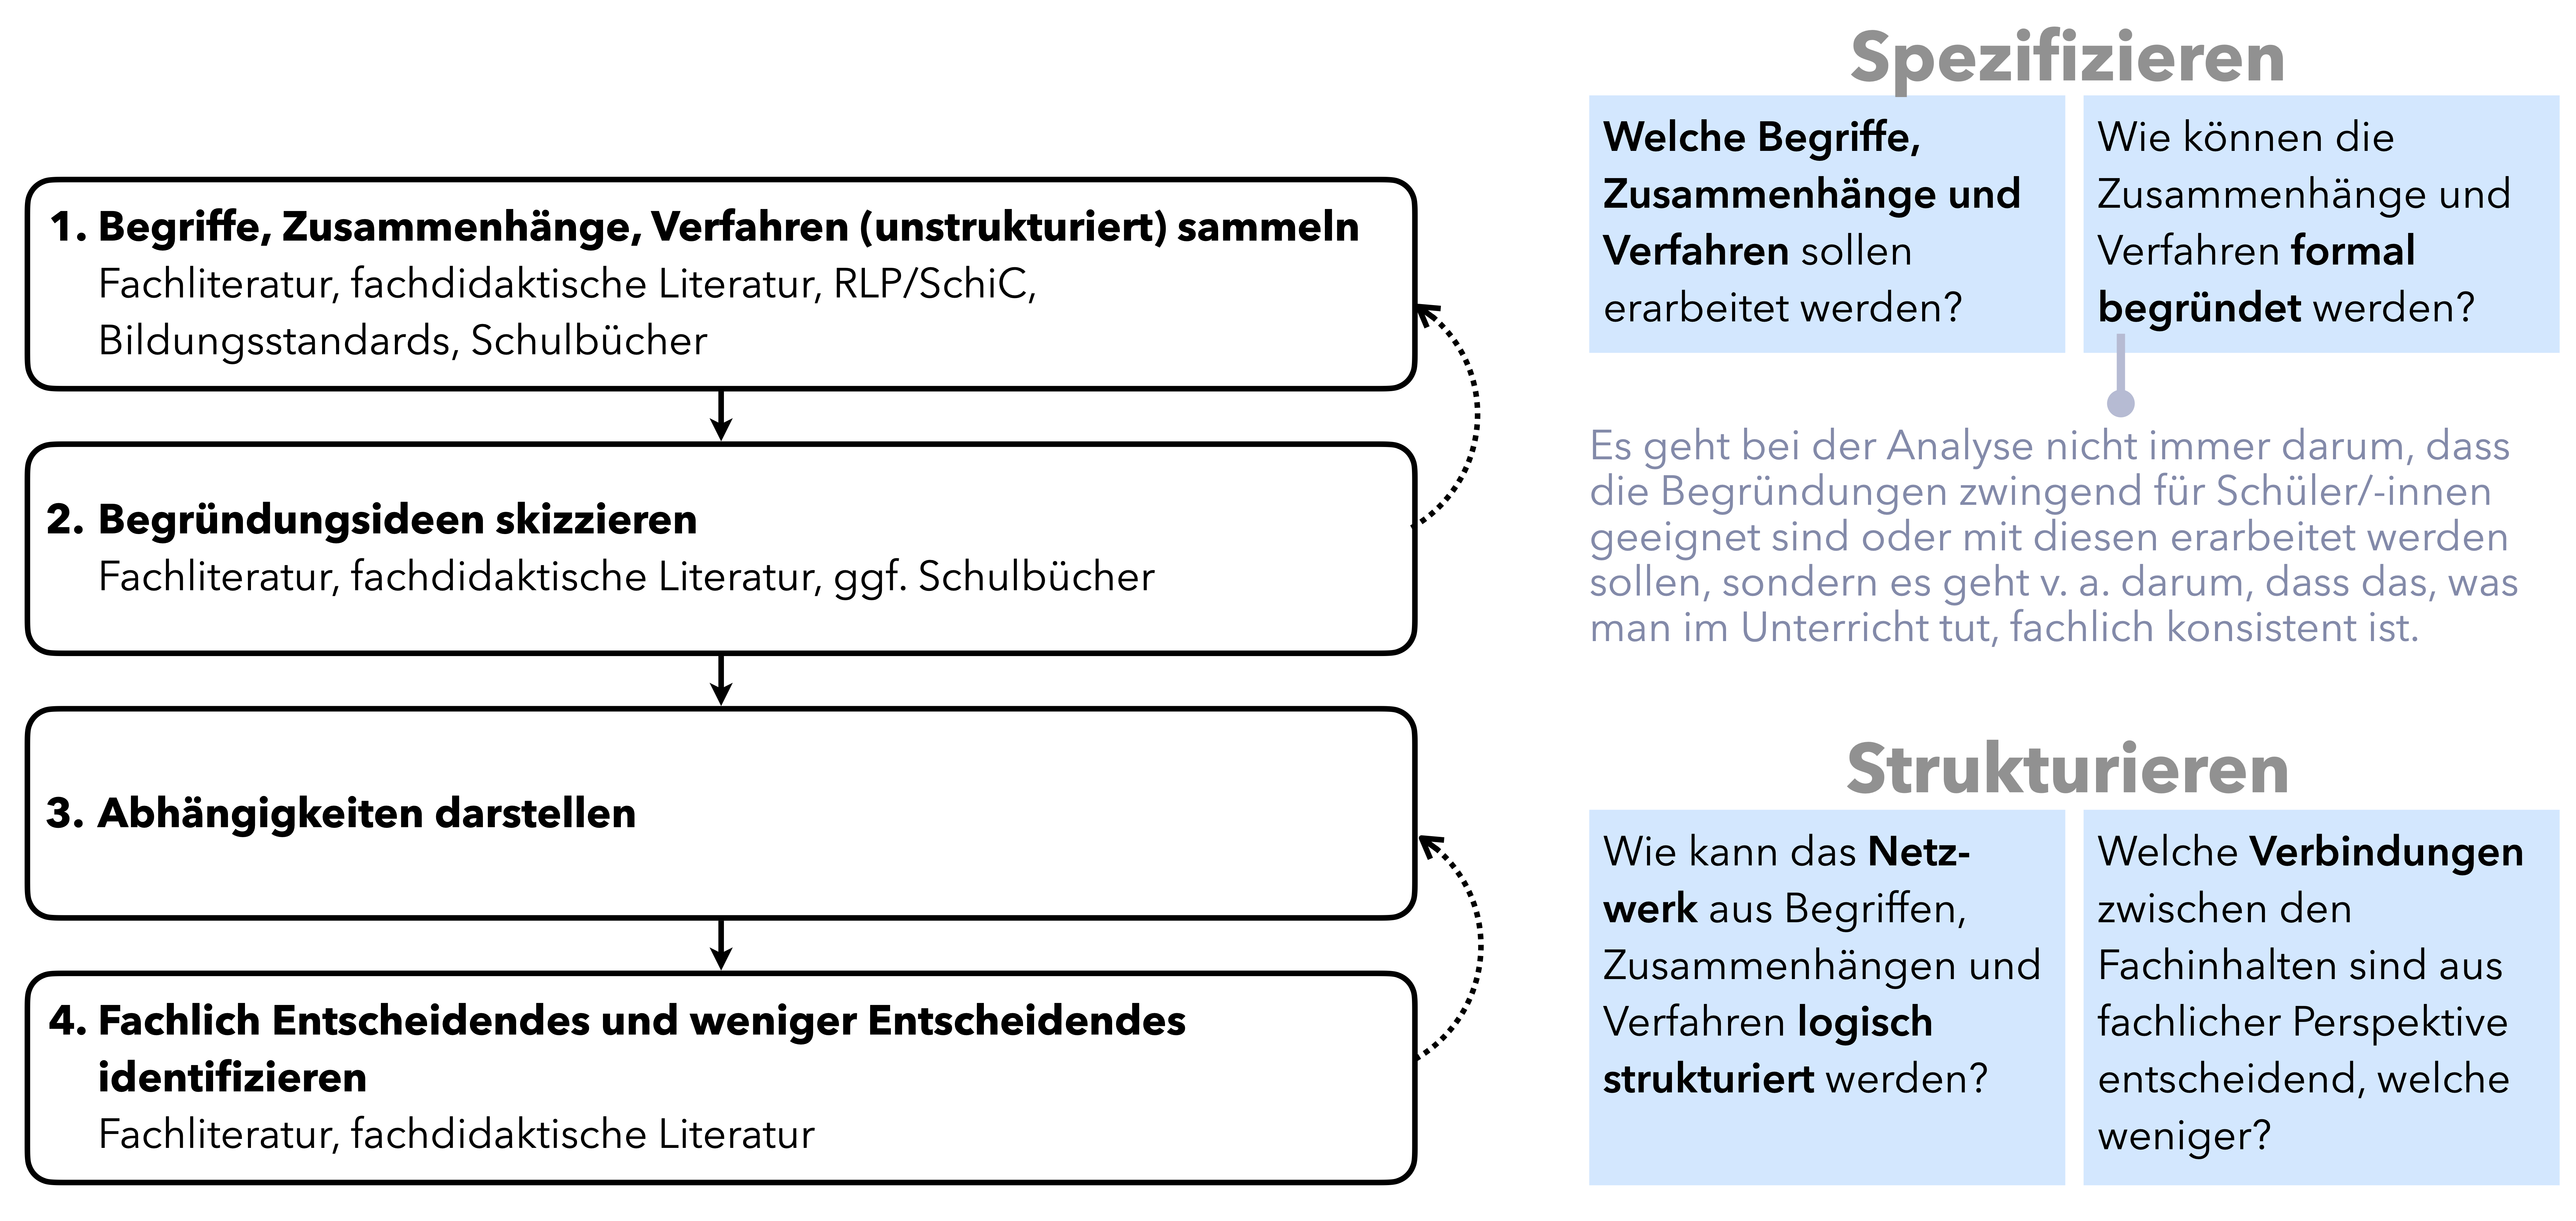
\includegraphics[width=0.9\linewidth]{pictures/B-OrientierungshilfeFormaleEbene} 

}

\caption{Orientierungshilfe zur formalen Ebene}\label{fig:OrientierungFormal}
\end{figure}

Die Übersicht kann als \href{files/Stoffdidaktik2024-OrientierungshilfeFormaleEbene.pdf}{pdf-Datei} heruntergeladen werden.

\section{Lernprozesse auslösen}\label{orientierungshilfe-lernprozesse-ausloesen}

Die Orientierungshilfe beschreibt eine Möglichkeit, die Motivierung und Zielbildung im Mathematikunterricht zu gestalten, um Lernprozesse auszulösen.

\begin{figure}

{\centering 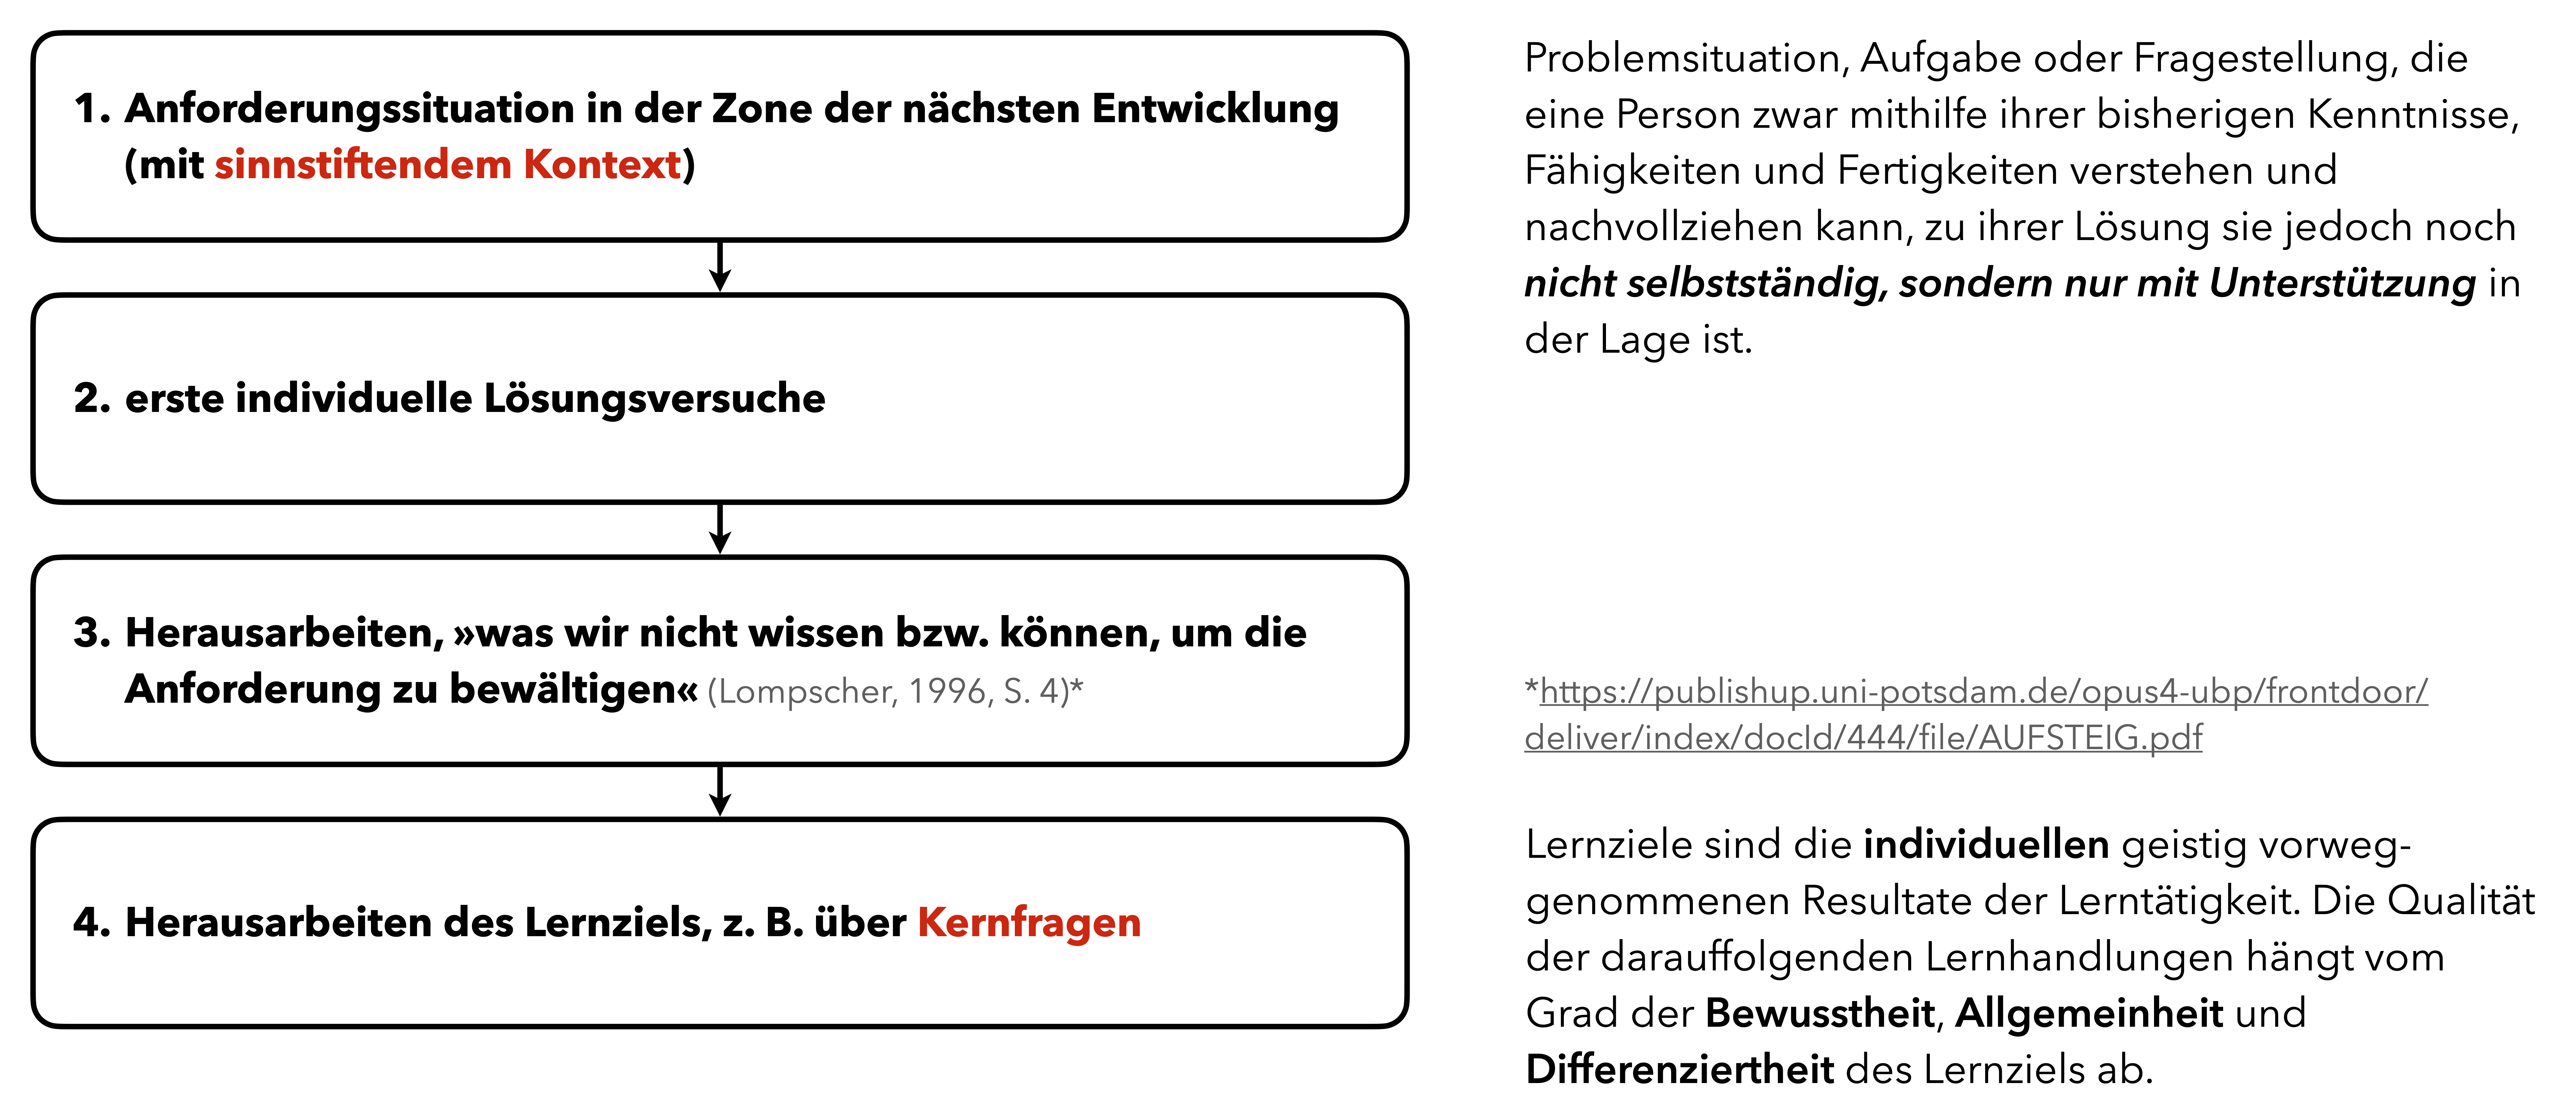
\includegraphics[width=0.9\linewidth]{pictures/B-OrientierungshilfeLernprozesseAusloesen} 

}

\caption{Orientierungshilfe zum Auslösen von Lernprozessen}\label{fig:OrientierungAusloesen}
\end{figure}

Die Übersicht kann als \href{files/Stoffdidaktik2024-OrientierungshilfeLernprozesseAusloesen.pdf}{pdf-Datei} heruntergeladen werden.

\chapter{Quellenarbeit}\label{quellenarbeit}

Um Ihre Recherche nach geeigneter fachdidaktischer Literatur zu unterstützen, sollen an dieser Stelle einige Hinweise zur Quellenarbeit gegeben werden.

\begin{itemize}
\item
  Auf der Webseite \url{https://juergen-roth.de/zeitschriften/} finden Sie eine Übersicht über \textbf{mathematikdidaktische Zeitschriften}. Als besonders geeignet für unterrichtspraktische und zugleich theoretisch fundierte Ideen soll die Zeitschrift \textbf{\emph{mathematik lehren}} empfohlen werden. Einen Themenüberblick bietet die Seite \url{https://juergen-roth.de/zeitschriften/mathematik-lehren/}, die Universitätsbibliothek Potsdam (\url{https://opac.ub.uni-potsdam.de}) verfügt über nahezu alle Ausgaben.\footnote{Bei der Suche nach dem Standort der Zeitschrift sollten Sie in der Recherche nach Zeitschriften filtern.} Auf der Webseite des Zeitschriftenverlags (\url{https://www.friedrich-verlag.de}) können Sie eine Stichwortsuche durchführen, so dass sie auch erfahren, in welchen Ausgaben einzelne Artikel enthalten sind.
\item
  Über die Webseite \url{https://eldorado.tu-dortmund.de} gelangen Sie an die \textbf{\emph{Beiträge zum Mathematikunterricht}} (BzMU). Dies sind Sammelbände, die jährlich zur Tagung der Gesellschaft für Didaktik der Mathematik (GDM) herausgegeben werden, bei der sich nahezu die komplette mathematikdidaktische Community im deutschsprachigen Raum trifft. Die Beiträge haben i.~d.~R. nur eine Länge von vier Seiten und geben einen kurzen Überblick über aktuelle Forschungsthemen. Am sinnvollsten erscheint eine Stichwortsuche über die Webseite. Die Beiträge selbst durchlaufen jedoch keinen \emph{Review-Prozess}, es kann also nicht per se eine Aussage über deren Qualität getroffen werden.
\item
  Aus dem universitätsinternen Netz bietet \url{https://link.springer.com} eine große Auswahl an \textbf{Monographien und Zeitschriften}. Einige der bei \url{https://juergen-roth.de/zeitschriften/} dargestellten Zeitschriften werden über Springer vertrieben.
\item
  Über die Seite \url{https://www.fachportal-paedagogik.de} können Sie zu den von Ihnen präferierten Stichworten Beiträge finden, die dort auch kurz zusammengefasst werden. Dies ist inbesondere für kurze \textbf{Überblicksrecherchen} sinnvoll. Die Verfügbarkeit der entsprechenden Beiträge wird dann über das Fachportal dargestellt.
\item
  Inbesondere \textbf{digital zugängliche Publikationen} lassen sich über die Webseite \url{https://www.base-search.net} recherchieren. Eine ähnliche Funktionalität, aber eher international orientiert, bietet die Seite \url{https://eric.ed.gov}.
\end{itemize}

\chapter{Vollständiges Literaturverzeichnis}\label{vollstuxe4ndiges-literaturverzeichnis}

\phantomsection\label{refs}
\begin{CSLReferences}{1}{0}
\bibitem[\citeproctext]{ref-Ableitinger2013}
Ableitinger, C., Kramer, J., \& Prediger, S. (Hrsg.). (2013). \emph{Zur doppelten {Diskontinuität} in der {Gymnasiallehrerbildung}: {Ansätze} zu {Verknüpfungen} der fachinhaltlichen {Ausbildung} mit schulischen {Vorerfahrungen} und {Erfordernissen}}. Springer Fachmedien Wiesbaden. \url{https://doi.org/10.1007/978-3-658-01360-8}

\bibitem[\citeproctext]{ref-Beutelspacher2012}
Beutelspacher, A., Danckwerts, R., Nickel, G., Spies, S., \& Wickel, G. (2012). \emph{Mathematik {Neu} {Denken}}. Vieweg+Teubner Verlag. \url{https://doi.org/10.1007/978-3-8348-8250-9}

\bibitem[\citeproctext]{ref-Boeer2014}
Böer, H., Göckel, D., Kliemann, S., Koepsell, A., Puscher, R., Schmidt, W., \& Vernay, R. (2014). \emph{Mathe live. 8, {Schülerbuch}} (1. Aufl.). Klett.

\bibitem[\citeproctext]{ref-Bruckler:2018}
Brückler, F. M. (2018). \emph{Geschichte der {Mathematik} kompakt: {Das} {Wichtigste} aus {Analysis}, {Wahrscheinlichkeitstheorie}, angewandter {Mathematik}, {Topologie} und {Mengenlehre}}. Springer Spektrum. \url{https://doi.org/10.1007/978-3-662-55574-3}

\bibitem[\citeproctext]{ref-Bruder2008b}
Bruder, R. (2008). Üben mit {Konzept}. \emph{mathematik lehren}, \emph{147}, 4--11.

\bibitem[\citeproctext]{ref-Bruder1989}
Bruder, R., \& Brückner, A. (1989). Zur {Beschreibung} von {Schülertätigkeiten} im {Mathematikunterricht} -- ein allgemeiner {Ansatz}. \emph{Pädagogische Forschung. Wissenschaftliche Nachrichten}, \emph{30}(6), 72--82.

\bibitem[\citeproctext]{ref-Bruner:1976}
Bruner, J. S. (1976). Die {Bedeutung} der {Struktur} im {Lernprozeß}. In A. Holtmann (Hrsg.), \emph{Das sozialwissenschaftliche {Curriculum} in der {Schule}: {Neue} {Formen} und {Inhalte}} (S. 77--90). VS Verlag für Sozialwissenschaften. \url{https://doi.org/10.1007/978-3-322-85275-5}

\bibitem[\citeproctext]{ref-Danckwerts:1988}
Danckwerts, R. (1988). Linearität als organisierendes Element zentraler Inhalte der Schulmathematik. \emph{Didaktik der Mathematik}, \emph{16}(2), 149--160.

\bibitem[\citeproctext]{ref-Danckwerts2013}
Danckwerts, R. (2013). Angehende {Gymnasiallehrer}(innen) brauchen eine „{Schulmathematik} vom höheren {Standpunkt}``! In C. Ableitinger, J. Kramer, \& S. Prediger (Hrsg.), \emph{Zur doppelten {Diskontinuität} in der {Gymnasiallehrerbildung}} (S. 77--94). Springer Fachmedien Wiesbaden. \url{https://doi.org/10.1007/978-3-658-01360-8_5}

\bibitem[\citeproctext]{ref-Etzold:2019}
Etzold, H. (2019a). \emph{Winkel-{Farm}} (Version 2) {[}App{]}. \url{https://apps.apple.com/de/app/winkel-farm/id1369585218}

\bibitem[\citeproctext]{ref-Etzold:2019Praxis4}
Etzold, H. (2019b). \emph{Winkel-{Farm} -- {Leitfaden} für {Lehrerinnen} und {Lehrer}} (Version 2). Zenodo. \url{https://doi.org/10.5281/zenodo.4747700}

\bibitem[\citeproctext]{ref-Etzold2021}
Etzold, H. (2021). \emph{Neue Zugänge zum Winkelbegriff} {[}Dissertation, Universität Potsdam{]}. \url{https://doi.org/10.25932/publishup-50418}

\bibitem[\citeproctext]{ref-Feldt-Caesar2017}
Feldt-Caesar, N. (2017). \emph{Konzeptualisierung und {Diagnose} von mathematischem {Grundwissen} und {Grundkönnen}}. Springer Fachmedien Wiesbaden. \url{https://doi.org/10.1007/978-3-658-17373-9}

\bibitem[\citeproctext]{ref-Freudenthal1973c}
Freudenthal, H. (1973a). \emph{Mathematics as an {Educational} {Task}}. Springer Netherlands. \url{https://doi.org/10.1007/978-94-010-2903-2}

\bibitem[\citeproctext]{ref-Freudenthal1973a}
Freudenthal, H. (1973c). \emph{Mathematik als pädagogische {Aufgabe}} (Bd. 1). Klett.

\bibitem[\citeproctext]{ref-Freudenthal:1973}
Freudenthal, H. (1973b). \emph{Mathematik als pädagogische {Aufgabe}} (Bd. 2). Klett.

\bibitem[\citeproctext]{ref-Gellert1986}
Gellert, W., Küstner, H., Hellwich, M., Kästner, H., \& Reichardt, H. (Hrsg.). (1986). \emph{Kleine {Enzyklopädie} {Mathematik}} (13. Aufl.). VEB Bibliographisches Institut.

\bibitem[\citeproctext]{ref-Giest2016a}
Giest, H. (2016). Kulturhistorische {Didaktik} und {Bildungstheorie}. \emph{Tätigkeitstheorie. Journal für tätigkeitstheoretische Forschung in Deutschland}, \emph{14}, 24--48. \url{http://www.ich-sciences.de/media/journal/Ausgabe_14/heft_14.pdf}

\bibitem[\citeproctext]{ref-Giest2006}
Giest, H., \& Lompscher, J. (2006). \emph{Lerntätigkeit -- {Lernen} aus kultur-historischer {Perspektive}. {Ein} {Beitrag} zur {Entwicklung} einer neuen {Lernkultur} im {Unterricht}}. Lehmanns Media.

\bibitem[\citeproctext]{ref-Greefrath2016}
Greefrath, G., Oldenburg, R., Siller, H.-S., Ulm, V., \& Weigand, H.-G. (2016). \emph{Didaktik der {Analysis}. {Aspekte} und {Grundvorstellungen} zentraler {Begriffe}} (F. Padberg \& A. Büchter, Hrsg.; 4. Aufl.). Springer Spektrum. \url{https://doi.org/10.1007/978-3-662-48877-5}

\bibitem[\citeproctext]{ref-Hefendehl-Hebeker:2016}
Hefendehl-Hebeker, L. (2016). Subject-matter didactics in {German} traditions: {Early} historical developments. \emph{Journal für Mathematik-Didaktik}, \emph{37}(S1), 11--31. \url{https://doi.org/10.1007/s13138-016-0103-7}

\bibitem[\citeproctext]{ref-Henn2015}
Henn, H.-W., \& Filler, A. (2015). \emph{Didaktik der {Analytischen} {Geometrie} und {Linearen} {Algebra}: {Algebraisch} verstehen -- {Geometrisch} veranschaulichen und anwenden}. Springer Spektrum.

\bibitem[\citeproctext]{ref-Hussmann:2016}
Hußmann, S., \& Prediger, S. (2016). Specifying and Structuring Mathematical Topics: A Four-Level Approach for Combining Formal, Semantic, Concrete, and Empirical Levels Exemplified for Exponential Growth. \emph{Journal für Mathematik-Didaktik}, \emph{37}(S1), 33--67. \url{https://doi.org/10.1007/s13138-016-0102-8}

\bibitem[\citeproctext]{ref-Hussmann:2016a}
Hußmann, S., Rezat, S., \& Sträßer, R. (2016). Subject {Matter} {Didactics} in {Mathematics} {Education}. \emph{Journal für Mathematik-Didaktik}, \emph{37}(S1), 1--9. \url{https://doi.org/10.1007/s13138-016-0105-5}

\bibitem[\citeproctext]{ref-Jahnke:2010}
Jahnke, T. (2010). Vom mählichen {Verschwinden} des {Fachs} aus der {Mathematikdidaktik}. \emph{GDM-Mitteilungen 89}, 21--24. \url{https://ojs.didaktik-der-mathematik.de/index.php/mgdm/article/view/559/550}

\bibitem[\citeproctext]{ref-Klein1925}
Klein, F. (1925). \emph{Elementarmathematik vom {Höheren} {Standpunkte} aus {II}. {Geometrie}}. Springer Berlin Heidelberg. \url{https://doi.org/10.1007/978-3-642-90852-1}

\bibitem[\citeproctext]{ref-Klein1955}
Klein, F. (1955). \emph{Elementarmathematik vom {Höheren} {Standpunkte} aus {III}. {Präzisions}- und {Approximationsmathematik}} (C. H. Müller, Hrsg.). Springer Berlin Heidelberg. \url{https://doi.org/10.1007/978-3-662-00246-9}

\bibitem[\citeproctext]{ref-Klein1967}
Klein, F. (1967). \emph{Elementarmathematik vom {Höheren} {Standpunkte} aus {I}. {Arithmetik}, {Algebra}, {Analysis}}. Springer Berlin Heidelberg. \url{https://doi.org/10.1007/978-3-662-11652-4}

\bibitem[\citeproctext]{ref-Krainer:1989}
Krainer, K. (1989). \emph{Lebendige {Geometrie}. Überlegungen zu einem integrativen {Verständnis} von {Geometrieunterricht} anhand des {Winkelbegriffs}} {[}Dissertation{]}. Alpen-Adria-Universität Klagenfurt.

\bibitem[\citeproctext]{ref-Krauthausen:2018}
Krauthausen, G. (2018). \emph{Einführung in die {Mathematikdidaktik}} (F. Padberg \& A. Büchter, Hrsg.; Mathematik Primarstufe und Sekundarstufe I + II). Springer Spektrum. \url{https://doi.org/10.1007/978-3-662-54692-5}

\bibitem[\citeproctext]{ref-Kruger2015}
Krüger, K., Sill, H.-D., \& Sikora, C. (2015). \emph{Didaktik der {Stochastik} in der {Sekundarstufe} {I}}. Springer Berlin Heidelberg. \url{https://doi.org/10.1007/978-3-662-43355-3}

\bibitem[\citeproctext]{ref-Lambert:2012}
Lambert, A. (2012). \emph{Gedanken zum aktuellen {Kompetenzbegriff} für den ({Mathematik}-)unterricht} {[}Vortrag{]}. Eingangsstatement zur Podiumsdiskussion im Rahmen des 3. Fachdidaktischen Kolloquiums an der Universität des Saarlandes, Saarbrücken. \url{https://www.uni-saarland.de/fileadmin/upload/einrichtung/zfl/PDF_Fachdidaktik/PDF_Kolloquium_FD/Kompetenzbegriff_für_den_Mathematikunterricht_Statement_mit_Folien.pdf}

\bibitem[\citeproctext]{ref-Leuders2011}
Leuders, T., Hußmann, S., Barzel, B., \& Prediger, S. (2011). Das macht {Sinn}! {Sinnstiftung} mit {Kontexten} und {Kernideen}. \emph{Praxis der Mathematik in der Schule}, \emph{53}(37), 2--9. \url{https://www.researchgate.net/publication/233978329}

\bibitem[\citeproctext]{ref-Lompscher1985b}
Lompscher, J. (1985). Die {Lerntätigkeit} als dominierende {Tätigkeit} des jüngeren {Schülers}. In J. Lompscher (Hrsg.), \emph{Persönlichkeitsentwicklung in der {Lerntätigkeit}} (S. 23--52). Volk und Wissen.

\bibitem[\citeproctext]{ref-Lompscher1996}
Lompscher, J. (1996). \emph{Aufsteigen vom {Abstrakten} zum {Konkreten} - {Lernen} und {Lehren} in {Zonen} der nächsten {Entwicklung}}. \url{https://publishup.uni-potsdam.de/opus4-ubp/frontdoor/deliver/index/docId/444/file/AUFSTEIG.pdf}

\bibitem[\citeproctext]{ref-Mienert2011}
Mienert, M., \& Pitcher, S. (2011). \emph{Pädagogische {Psychologie}}. VS Verlag für Sozialwissenschaften. \url{https://doi.org/10.1007/978-3-531-92095-5}

\bibitem[\citeproctext]{ref-MinisteriumfurBildungJugendundSportdesLandesBrandenburg2022}
Ministerium für Bildung, Jugend und Sport des Landes Brandenburg (Hrsg.). (2022). \emph{Rahmenlehrplan für die gymnasiale {Oberstufe}. {Teil} {C}. {Mathematik}}. \url{https://bildungsserver.berlin-brandenburg.de/fileadmin/bbb/unterricht/rahmenlehrplaene/gymnasiale_oberstufe/curricula/2022/Teil_C_RLP_GOST_2022_Mathematik.pdf}

\bibitem[\citeproctext]{ref-MinisteriumfuerBildungJugendundSportdesLandesBrandenburg2023}
Ministerium für Bildung, Jugend und Sport des Landes Brandenburg (Hrsg.). (2023). \emph{Rahmenlehrplan {Brandenburg}. {Teil} {C}, {Mathematik}, {Jahrgangsstufen} 1~--~10}. \url{https://bildungsserver.berlin-brandenburg.de/fileadmin/bbb/unterricht/rahmenlehrplaene/Rahmenlehrplanprojekt/amtliche_Fassung/getrennt_2023/BB_RLP_2023_Teil_C_Ma_GenF_1.pdf}

\bibitem[\citeproctext]{ref-Mitchelmore:1990}
Mitchelmore, M. (1990). Psychologische und mathematische Schwierigkeiten beim Lernen des Winkelbegriffs. \emph{mathematica didactica}, \emph{13}, 19--37.

\bibitem[\citeproctext]{ref-Mitchelmore:1998}
Mitchelmore, M., \& White, P. (1998). Development of {Angle} {Concepts}: {A} {Framework} for {Research}. \emph{Mathematics Education Research Journal}, \emph{10}(3), 4--27.

\bibitem[\citeproctext]{ref-Padberg:2017}
Padberg, F., \& Wartha, S. (2017). \emph{Didaktik der {Bruchrechnung}} (5. Aufl.). Springer Spektrum. \url{https://doi.org/10.1007/978-3-662-52969-0}

\bibitem[\citeproctext]{ref-Reitz-Koncebovski2018}
Reitz-Koncebovski, K., Kortenkamp, U., \& Goral, J. (2018). Gestaltungsprinzipien für fachwissenschaftliche {Einführungsveranstaltungen}. In A. Borowski, A. Ehlert, \& H. Prechtl (Hrsg.), \emph{{PSI}-{Potsdam}. {Ergebnisbericht} zu den {Aktivitäten} im {Rahmen} der {Qualitätsoffensive} {Lehrerbildung} (2015-2018)} (S. 175--188). Universitätsverlag Potsdam. \url{https://nbn-resolving.org/urn:nbn:de:kobv:517-opus4-420301}

\bibitem[\citeproctext]{ref-Richter2016}
Richter, K., \& Bruder, R. (2016). Das {Tätigkeitskonzept} als {Analyseinstrument} für technologiegestützte {Lernprozesse} im {Fach} {Mathematik}. In G. Heintz, H.-J. Elschenbroich, G. Pinkernell, \& F. Schacht (Hrsg.), \emph{Digitale {Werkzeuge} für den {Mathematikunterricht}: {Festschrift} für {Hans}-{Jürgen} {Elschenbroich}} (1. Auflage, S. 188--214). Verlag Klaus Seeberger.

\bibitem[\citeproctext]{ref-Salle2021}
Salle, A., \& Clüver, T. (2021). Herleitung von {Grundvorstellungen} als normative {Leitlinien} -- {Beschreibung} eines theoriebasierten {Verfahrensrahmens}. \emph{Journal für Mathematik-Didaktik}. \url{https://doi.org/10.1007/s13138-021-00184-5}

\bibitem[\citeproctext]{ref-Schecker2018}
Schecker, H., Wilhelm, T., Hopf, M., \& Duit, R. (Hrsg.). (2018). \emph{Schülervorstellungen und {Physikunterricht}: {Ein} {Lehrbuch} für {Studium}, {Referendariat} und {Unterrichtspraxis}}. Springer Berlin Heidelberg. \url{https://doi.org/10.1007/978-3-662-57270-2}

\bibitem[\citeproctext]{ref-Schubert:2011}
Schubert, S., \& Schwill, A. (2011). \emph{Didaktik der {Informatik}} (2. Aufl). Spektrum, Akad. Verl. \url{https://doi.org/10.1007/978-3-8274-2653-6}

\bibitem[\citeproctext]{ref-Schupp:2016}
Schupp, H. (2016). Gedanken zum „{Stoff}`` und zur „{Stoffdidaktik}`` sowie zu ihrer {Bedeutung} für die {Qualität} des {Mathematikunterrichts}. \emph{Mathematische Semesterberichte}, \emph{63}(1), 69--92. \url{https://doi.org/10.1007/s00591-016-0159-y}

\bibitem[\citeproctext]{ref-Schwill:1994}
Schwill, A. (1994). \emph{Fundamentale {Ideen} in {Mathematik} und {Informatik}}. Herbsttagung des Arbeitskreises Mathematikunterricht und Informatik, Wolfenbüttel. \url{http://www.informatikdidaktik.de/didaktik/Forschung/Wolfenbuettel94.pdf}

\bibitem[\citeproctext]{ref-KMK:2012}
Sekretariat der Ständigen Konferenz der Kultusminister der Länder in der Bundesrepublik Deutschland. (2012). \emph{Bildungsstandards im {Fach} {Mathematik} für die {Allgemeine} {Hochschulreife}. (Beschluss der Kultusministerkonferenz vom 18.10.2012)}. \url{https://www.kmk.org/fileadmin/Dateien/veroeffentlichungen_beschluesse/2012/2012_10_18-Bildungsstandards-Mathe-Abi.pdf}

\bibitem[\citeproctext]{ref-SekretariatderStandigenKonferenzderKultusministerderLanderinderBundesrepublikDeutschland2022}
Sekretariat der Ständigen Konferenz der Kultusminister der Länder in der Bundesrepublik Deutschland. (2022a). \emph{Bildungsstandards für das {Fach} {Mathematik} {Erster} {Schulabschluss} ({ESA}) und {Mittlerer} {Schulabschluss} ({MSA}). ({Beschluss} der {Kultusministerkonferenz} vom 15.10.2004 und vom 04.12.2003, i.d.{F}. vom 23.06.2022)}. \url{https://www.kmk.org/fileadmin/Dateien/veroeffentlichungen_beschluesse/2022/2022_06_23-Bista-ESA-MSA-Mathe.pdf}

\bibitem[\citeproctext]{ref-SekretariatderStandigenKonferenzderKultusministerderLanderinderBundesrepublikDeutschland2022a}
Sekretariat der Ständigen Konferenz der Kultusminister der Länder in der Bundesrepublik Deutschland. (2022b). \emph{Bildungsstandards für das {Fach} {Mathematik} {Primarbereich}. ({Beschluss} der {Kultusministerkonferenz} vom 15.10.2004, i.d.{F}. vom 23.06.2022)}. \url{https://www.kmk.org/fileadmin/Dateien/veroeffentlichungen_beschluesse/2022/2022_06_23-Bista-Primarbereich-Mathe.pdf}

\bibitem[\citeproctext]{ref-Steinhofel1988}
Steinhöfel, W., Reichold, K., \& Frenzel, L. (1988). \emph{Zur {Gestaltung} typischer {Unterrichtssituationen} im {Mathematikunterricht}}. Ministerium für Volksbildung.

\bibitem[\citeproctext]{ref-Strehl:1983}
Strehl, R. (1983). Anschauliche {Vorstellung} und mathematische {Theorie} beim {Winkelbegriff}. \emph{mathematica didactica}, \emph{6}, 129--146.

\bibitem[\citeproctext]{ref-Taylor:1715}
Taylor, B. (1715). \emph{Linear perspective}. printed for R. Knaplock at the Bishop's-Head in St. Paul's Church-Yard. \url{https://nl.sub.uni-goettingen.de/id/0590700700}

\bibitem[\citeproctext]{ref-Thiel-Schneider2018}
Thiel-Schneider, A. (2018). \emph{Zum {Begriff} des exponentiellen {Wachstums}}. Springer Fachmedien Wiesbaden. \url{https://doi.org/10.1007/978-3-658-21895-9}

\bibitem[\citeproctext]{ref-Tietze:2000a}
Tietze, U.-P., Klika, M., \& Wolpers, H. (Hrsg.). (2000a). \emph{Mathematikunterricht in der {Sekundarstufe} {II}. {Band} 1: {Fachdidaktische} {Grundfragen}, {Didaktik} der {Analysis}} (2. Aufl.). Vieweg+Teubner Verlag. \url{https://doi.org/10.1007/978-3-322-90568-0}

\bibitem[\citeproctext]{ref-Tietze:2000}
Tietze, U.-P., Klika, M., \& Wolpers, H. (Hrsg.). (2000b). \emph{Mathematikunterricht in der {Sekundarstufe} {II}. {Band} 2: {Didaktik} der {Analytischen} {Geometrie} und {Linearen} {Algebra}}. Vieweg+Teubner Verlag. \url{https://doi.org/10.1007/978-3-322-86479-6}

\bibitem[\citeproctext]{ref-Tietze:2002}
Tietze, U.-P., Klika, M., \& Wolpers, H. (Hrsg.). (2002). \emph{Mathematikunterricht in der {Sekundarstufe} {II}. {Band} 3: {Didaktik} der {Stochastik}}. Vieweg+Teubner Verlag. \url{https://doi.org/10.1007/978-3-322-83144-6}

\bibitem[\citeproctext]{ref-vandenHeuvel-Panhuizen2003}
van den Heuvel-Panhuizen, M. (2003). The didactical use of models in realistic mathematics education: {An} example from a longitudinal trajectory on percentage. \emph{Educational Studies in Mathematics}, \emph{54}, 9--35. \url{https://doi.org/10.1023/B:EDUC.0000005212.03219.dc}

\bibitem[\citeproctext]{ref-Vohns:2000}
Vohns, A. (2000). \emph{Das {Messen} als fundamentale {Idee}} {[}1. Staatsexamensarbeit, Universität-Gesamthochschule Siegen{]}. \url{https://wwwu.aau.at/avohns/pdf/messen.pdf}

\bibitem[\citeproctext]{ref-Vollrath2012}
Vollrath, H.-J., \& Roth, J. (2012). \emph{Grundlagen des {Mathematikunterrichts} in der {Sekundarstufe}} (F. Padberg, Hrsg.; 2. Aufl.). Spektrum Akademischer Verlag. \url{https://doi.org/10.1007/978-3-8274-2855-4}

\bibitem[\citeproctext]{ref-Hofe:1995}
vom Hofe, R. (1995). \emph{Grundvorstellungen mathematischer {Inhalte}}. Spektrum Akademischer Verlag.

\bibitem[\citeproctext]{ref-vomHofe2014}
vom Hofe, R. (2014). Primäre und sekundäre {Grundvorstellungen}. In J. Roth \& J. Ames (Hrsg.), \emph{Beiträge zum {Mathematikunterricht} 2014, 48. {Jahrestagung} der {Gesellschaft} für {Didaktik} der {Mathematik} vom 10.03.2014 bis 14.03.2014 in {Koblenz}}. WTM. \url{https://doi.org/10.17877/DE290R-8808}

\bibitem[\citeproctext]{ref-vomHofe2014a}
vom Hofe, R., \& Hattermann, M. (2014). Zugänge zu negativen {Zahlen}. \emph{mathematik lehren}, 2--7.

\bibitem[\citeproctext]{ref-vonderBank:2013}
von der Bank, M.-C. (2013). Fundamentale {Ideen}, insbesondere {Optimierung}. In A. Filler \& M. Ludwig (Hrsg.), \emph{Wege zur {Begriffsbildung} für den {Geometrieunterricht}. {Ziele} und {Visionen} 2020. {Vorträge} auf der 29. {Herbsttagung} des {Arbeitskreises} {Geometrie} in der {Gesellschaft} für {Didaktik} der {Mathematik} vom 14. bis 16. {September} 2012 in {Saarbrücken}} (S. 83--124). Franzbecker. \url{https://www.math.uni-sb.de/service/lehramt/AKGeometrie/AKGeometrie2012.pdf}

\bibitem[\citeproctext]{ref-Bank:2016}
von der Bank, M.-C. (2016). \emph{Fundamentale {Ideen} der {Mathematik}: {Weiterentwicklung} einer {Theorie} zu deren unterrichtspraktischer {Nutzung}} {[}Dissertation, Universität des Saarlandes{]}. \url{https://doi.org/10.22028/D291-26673}

\bibitem[\citeproctext]{ref-Weigand2018}
Weigand, H.-G., Filler, A., Hölzl, R., Kuntze, S., Ludwig, M., Roth, J., Schmidt-Thieme, B., \& Wittmann, G. (2018). \emph{Didaktik der {Geometrie} für die {Sekundarstufe} {I}}. Springer Berlin Heidelberg. \url{https://doi.org/10.1007/978-3-662-56217-8}

\bibitem[\citeproctext]{ref-Weigand2022}
Weigand, H.-G., Schüler-Meyer, A., \& Pinkernell, G. (2022). \emph{Didaktik der {Algebra}: nach der {Vorlage} von {Hans}-{Joachim} {Vollrath}}. Springer Berlin Heidelberg. \url{https://doi.org/10.1007/978-3-662-64660-1}

\bibitem[\citeproctext]{ref-WikiPeano}
Wikipedia. (2021). \emph{Peano-Axiome --- Wikipedia{,} die freie Enzyklopädie}. \url{https://de.wikipedia.org/w/index.php?title=Peano-Axiome&oldid=216675163}

\bibitem[\citeproctext]{ref-WikiKerze}
Wikipedia. (2022a). \emph{Kerzenuhr --- Wikipedia{,} die freie Enzyklopädie}. \url{https://de.wikipedia.org/w/index.php?title=Kerzenuhr&oldid=227115991}

\bibitem[\citeproctext]{ref-dewiki:228417777}
Wikipedia. (2022b). \emph{Kultusministerkonferenz --- Wikipedia{,} die freie Enzyklopädie}. \url{https://de.wikipedia.org/w/index.php?title=Kultusministerkonferenz&oldid=228417777}

\bibitem[\citeproctext]{ref-Wittmann:2015}
Wittmann, E. C. (2015). Strukturgenetische didaktische {Analysen} -- empirische {Forschung} „erster {Art}``. \emph{mathematica didactica}, 239--255. \url{http://www.mathematica-didactica.com/altejahrgaenge/md_2015/md_2015_Wittmann_Stoffdidaktik.pdf}

\end{CSLReferences}

% \printindex

\end{document}
